\documentclass[journal, 9pt]{IEEEtran}
\usepackage{preamble}

\begin{document}
% \raggedbottom  % put this once (ideally in the main file after \begin{document})

% paper title
\title{Building a Knowledge-Graph Enhanced Literature Search Engine\\ \small{ESIPS Honours Progress Report}}

% author names 
\author{Jordan Lee Guyot, 510293372}% <-this % stops a space
        
% The report headers
\markboth{Latent Knowledge, \today}%do not delete next lines
{}

% make the title area
\maketitle

% \input{tex_files/0. Abstract/}

% Introduction section for the ESIPS honours thesis.
% Intended to be pulled into main.tex via % Introduction section for the ESIPS honours thesis.
% Intended to be pulled into main.tex via % Introduction section for the ESIPS honours thesis.
% Intended to be pulled into main.tex via \input{introduction} (or \include).
% Assumes an IEEEtran two-column document; contains no preamble.
% Section cross-references use \ref{} to auto-numbered labels. The one exception is
% the Conclusion (Section~VI), left as a literal numeral until that section is written
% and wired into main.tex; see the PLACEHOLDER note at the end of this file.

\section{Introduction}
\label{sec:intro}

A literature search asks two things of a retrieval system: firstly, to find papers that precisely match a set of stated constraints; secondly, to find papers that are about what the user means. These map onto two retrieval paradigms that have proven difficult to reconcile. Structured retrieval, being exact keyword and boolean matching over typed metadata, answers a query precisely, in that a paper either satisfies the constraints or it does not. Semantic retrieval, being dense vector embeddings that rank documents by meaning, recovers relevance that exact terms miss, but returns what lies nearest in a learned space rather than what provably matches. The two serve different needs. Assembling an exhaustive evidence base, as in a systematic review, demands the precision of the former, while exploring an unfamiliar area rewards the recall of the latter. Deployed literature-search engines force a choice between them.

The aim of this thesis is to develop a scholarly search system that can search based on nested entity queries, and semantic relationships via a three-stage mechanism: 1) Structured Graph Retrieval; 2) Bi-encoder semantic retrieval; 3) Cross-encoder semantic re-ranking. Accordingly, the three research questions that will form an answer to this include:

\begin{enumerate}
    \item To what extent can modern AI construct the artefacts required for deterministic structured graph retrieval of a candidate set of papers: the per-work keyword index extracted offline from the literature, and the intermediate representation formulated from the natural-language query;
    \item How well do current bi-encoders and cross-encoders perform on semantic ad-hoc search tasks on scientific retrieval benchmarks;
    \item How does the three-stage mechanism differ from existing systems, and what explains those differences?
\end{enumerate}

The remainder of this report is organised as follows. Section~\ref{sec:litreview} reviews the literature on scholarly retrieval, positioning the design against dense retrieval, graph-augmented methods, and structured-query translation, and surveying the systems and benchmarks currently available. Section~\ref{sec:research-design} presents the research design: the system architecture, the graph schema and ingestion pipeline, the design of each retrieval stage, and the methodology used to validate them. Section~\ref{sec:data-results} reports the outcome of each component benchmark, which Section~\ref{sec:analysis-discussion} then analyses against the three research questions. Section~VI draws conclusions and identifies future work.

% PLACEHOLDER (conclusion): 'Section~VI' above is left as a literal numeral because
% the Conclusion and Future Work section is not yet in the build. Replace it with
% Section~\ref{sec:conclusion} once that section is written and \input into main.tex. (or \include).
% Assumes an IEEEtran two-column document; contains no preamble.
% Section cross-references use \ref{} to auto-numbered labels. The one exception is
% the Conclusion (Section~VI), left as a literal numeral until that section is written
% and wired into main.tex; see the PLACEHOLDER note at the end of this file.

\section{Introduction}
\label{sec:intro}

A literature search asks two things of a retrieval system: firstly, to find papers that precisely match a set of stated constraints; secondly, to find papers that are about what the user means. These map onto two retrieval paradigms that have proven difficult to reconcile. Structured retrieval, being exact keyword and boolean matching over typed metadata, answers a query precisely, in that a paper either satisfies the constraints or it does not. Semantic retrieval, being dense vector embeddings that rank documents by meaning, recovers relevance that exact terms miss, but returns what lies nearest in a learned space rather than what provably matches. The two serve different needs. Assembling an exhaustive evidence base, as in a systematic review, demands the precision of the former, while exploring an unfamiliar area rewards the recall of the latter. Deployed literature-search engines force a choice between them.

The aim of this thesis is to develop a scholarly search system that can search based on nested entity queries, and semantic relationships via a three-stage mechanism: 1) Structured Graph Retrieval; 2) Bi-encoder semantic retrieval; 3) Cross-encoder semantic re-ranking. Accordingly, the three research questions that will form an answer to this include:

\begin{enumerate}
    \item To what extent can modern AI construct the artefacts required for deterministic structured graph retrieval of a candidate set of papers: the per-work keyword index extracted offline from the literature, and the intermediate representation formulated from the natural-language query;
    \item How well do current bi-encoders and cross-encoders perform on semantic ad-hoc search tasks on scientific retrieval benchmarks;
    \item How does the three-stage mechanism differ from existing systems, and what explains those differences?
\end{enumerate}

The remainder of this report is organised as follows. Section~\ref{sec:litreview} reviews the literature on scholarly retrieval, positioning the design against dense retrieval, graph-augmented methods, and structured-query translation, and surveying the systems and benchmarks currently available. Section~\ref{sec:research-design} presents the research design: the system architecture, the graph schema and ingestion pipeline, the design of each retrieval stage, and the methodology used to validate them. Section~\ref{sec:data-results} reports the outcome of each component benchmark, which Section~\ref{sec:analysis-discussion} then analyses against the three research questions. Section~VI draws conclusions and identifies future work.

% PLACEHOLDER (conclusion): 'Section~VI' above is left as a literal numeral because
% the Conclusion and Future Work section is not yet in the build. Replace it with
% Section~\ref{sec:conclusion} once that section is written and \input into main.tex. (or \include).
% Assumes an IEEEtran two-column document; contains no preamble.
% Section cross-references use \ref{} to auto-numbered labels. The one exception is
% the Conclusion (Section~VI), left as a literal numeral until that section is written
% and wired into main.tex; see the PLACEHOLDER note at the end of this file.

\section{Introduction}
\label{sec:intro}

A literature search asks two things of a retrieval system: firstly, to find papers that precisely match a set of stated constraints; secondly, to find papers that are about what the user means. These map onto two retrieval paradigms that have proven difficult to reconcile. Structured retrieval, being exact keyword and boolean matching over typed metadata, answers a query precisely, in that a paper either satisfies the constraints or it does not. Semantic retrieval, being dense vector embeddings that rank documents by meaning, recovers relevance that exact terms miss, but returns what lies nearest in a learned space rather than what provably matches. The two serve different needs. Assembling an exhaustive evidence base, as in a systematic review, demands the precision of the former, while exploring an unfamiliar area rewards the recall of the latter. Deployed literature-search engines force a choice between them.

The aim of this thesis is to develop a scholarly search system that can search based on nested entity queries, and semantic relationships via a three-stage mechanism: 1) Structured Graph Retrieval; 2) Bi-encoder semantic retrieval; 3) Cross-encoder semantic re-ranking. Accordingly, the three research questions that will form an answer to this include:

\begin{enumerate}
    \item To what extent can modern AI construct the artefacts required for deterministic structured graph retrieval of a candidate set of papers: the per-work keyword index extracted offline from the literature, and the intermediate representation formulated from the natural-language query;
    \item How well do current bi-encoders and cross-encoders perform on semantic ad-hoc search tasks on scientific retrieval benchmarks;
    \item How does the three-stage mechanism differ from existing systems, and what explains those differences?
\end{enumerate}

The remainder of this report is organised as follows. Section~\ref{sec:litreview} reviews the literature on scholarly retrieval, positioning the design against dense retrieval, graph-augmented methods, and structured-query translation, and surveying the systems and benchmarks currently available. Section~\ref{sec:research-design} presents the research design: the system architecture, the graph schema and ingestion pipeline, the design of each retrieval stage, and the methodology used to validate them. Section~\ref{sec:data-results} reports the outcome of each component benchmark, which Section~\ref{sec:analysis-discussion} then analyses against the three research questions. Section~VI draws conclusions and identifies future work.

% PLACEHOLDER (conclusion): 'Section~VI' above is left as a literal numeral because
% the Conclusion and Future Work section is not yet in the build. Replace it with
% Section~\ref{sec:conclusion} once that section is written and \input into main.tex.

\section{Literature Review}
\label{sec:litreview}

\subsection{History of Scholarly Search}
\label{sec:history}

Scholarly retrieval has navigated a recurring tension between structured
indexing (controlled vocabularies and typed metadata) and free-text retrieval
(full-content indexing), with each era layering onto the last rather than
swinging between them. Pre-digital catalogues and the early digital
bibliographic databases (MEDLARS, INSPEC, PsycINFO) were anchored to
controlled vocabularies and Boolean intermediaries, whose dominant failure
mode Lancaster diagnosed as vocabulary mismatch rather than algorithmic
weakness~\cite{lancaster1969medlars}. The web era sidestepped that mismatch by
indexing full text at scale through Google Scholar, Scopus, and BM25- and
PageRank-driven
ranking~\cite{robertson1994bm25,brin1998pagerank,falagas2008comparison}, at
the cost of the disciplined precision that controlled vocabularies had
guaranteed. Modern infrastructure (Semantic Scholar, OpenAlex,
OpenCitations) partially reintroduced typed metadata as a navigable layer over
web-scale
text~\cite{ammar2018construction,priem2022openalex,peroni2020opencitations},
and the post-2022 generation of LLM- and embedding-driven tools now sits on
top of those graphs. Each generation has therefore inherited the substrate
of the last, addressed its dominant limitation, and introduced a new one. The
methods examined in Section~\ref{sec:recent-advances}, namely dense
retrieval, graph augmentation, natural-language-to-structured-query
translation, and query reformulation, are best read as the field's current
attempt to reconcile these two paradigms rather than choose between them,
and this thesis takes that reconciliation as its starting point.

% =====================================================================
% Deep literature review: knowledge-graph-enhanced and hybrid scholarly
% search.  Assumes standard packages (hyperref, natbib or biblatex)
% and a bibliography file containing the keys used below.
% =====================================================================

\subsection{Recent research advances}
\label{sec:recent-advances}

This thesis takes a different stance toward each of the four threads
examined below.  Dense retrieval (Section~\ref{sec:lr-dense}) is retained
as one signal in a hybrid pipeline, since the strongest current models
still miss roughly a quarter of relevant papers on realistic scientific
queries.  Graph-augmented methods (Section~\ref{sec:lr-graph}) supply the
conceptual motivation for ingesting OpenAlex into a typed knowledge
graph but offer no benchmarked baseline to copy.  Structured-query
translation (Section~\ref{sec:lr-nl2q}) is the design this thesis
pursues, instantiated through an intermediate JSON representation that
decouples LLM-based intent extraction from deterministic query
compilation.  Reformulation (Section~\ref{sec:lr-rag}) is set aside, both
because it degrades strong retrievers and because it cannot express the
structural queries a typed graph makes available.

\subsubsection{Scholarly embeddings and dense retrieval for scientific text}
\label{sec:lr-dense}

Dense retrieval is retained as one signal in this thesis's hybrid
pipeline rather than its primary mechanism, because the strongest current
models still miss roughly a quarter of relevant papers on realistic
scientific queries.  Three lines of progress have improved dense
retrieval without closing this gap.  Wider training distributions, from
DPR \cite{karpukhin2020dpr} through unsupervised contrastive
pre-training \cite{izacard2022contriever} and weakly-supervised pairs at
$10^8$--$10^9$ scale \cite{wang2022e5,li2023gte,xiao2023cpack,chen2024bgem3},
have lifted average nDCG@10 on BEIR \cite{thakur2021beir} but left a
structural weakness on entity-heavy and lexical queries.  Late
interaction \cite{khattab2020colbert,santhanam2022colbertv2} and learned
sparse retrieval \cite{formal2021splade,formal2022splade} preserved
fine-grained query-document interaction at modest cost, with ColBERTv2
reaching a BEIR nDCG@10 average of 49.9 across thirteen datasets while
shrinking the index by a factor of 6--10 \cite{santhanam2022colbertv2}.
Scholarly-domain encoders pursued the orthogonal axis of citation
supervision \cite{beltagy2019scibert,cohan2020specter,ostendorff2022scincl},
but Singh et al.'s 24-task SciRepEval benchmark
\cite{singh2023scirepeval} shows that proximity-trained representations
do not transfer to classification or ad-hoc search.  Their adapter-based
SPECTER2 reaches MAP 38.4 and Recall@5 33.0 on MDCR against BM25's 33.7
and 28.5, suggesting single-vector citation-trained encoders are not
sufficient for heterogeneous scholarly tasks.

The strongest empirical evidence that dense retrieval remains unsolved
on scientific text is LitSearch \cite{ajith2024litsearch}.  Ajith et al.\
assembled 597 realistic literature-search questions paired against a
corpus of 64,183 papers, half rewritten from inline citations and half
written by the papers' own authors.  None of the systems perform well.
The best open model tested, GritLM-7B, reaches Recall@5 of 74.8 on
specific questions but falls to 67.7 on the inline-citation subset, which
deliberately filters for low title-abstract lexical overlap, and to
Recall@20 of 70.8 on broad questions.  Commercial tools score 17.5
Recall@5 on author-written specific questions, roughly 65 points below
GritLM-7B.  The cross-benchmark contrast makes the diagnosis concrete:
GritLM-7B scores 70.3 nDCG@10 on Natural Questions but only 44.1 on broad
LitSearch, a 26-point drop that cannot be explained by random noise.
LitSearch also surfaces three failure modes that single-vector dense
retrieval cannot easily address.  Inline-citation queries are
systematically harder than author-written ones because authors reuse
their own title and abstract vocabulary, and retrievers exploit this
lexical shortcut.  Broad questions remain harder than specific ones.
Feeding full text rather than title and abstract to GritLM hurts
retrieval on author-written specific queries (Recall@5 drops from 82.5 to
73.0), which Ajith et al.\ attribute to a distributional mismatch between
training (MS~MARCO passages around 60 tokens) and full scientific texts.
Related work reinforces the picture.  DORIS-MAE \cite{wang2023dorismae}
reports that general-purpose models modestly outperform most
scholarly-specific ones on multi-aspect CS queries, and CSFCube
\cite{mysore2021csfcube} shows that SPECTER's performance varies
substantially across facets.  Notably, LitSearch does not benchmark
SPECTER2 or SciNCL in its main tables.  Combined with the DORIS-MAE
findings, this strongly suggests that citation-triplet-trained encoders
have not been shown to outperform strong general-purpose retrievers on
realistic natural-language literature search.  They remain the models of
choice for paper-paper similarity, but that is a different task.

These structural failures, on broad questions, multi-hop intent, and
typed-relation queries that single-vector representations cannot express,
are precisely what motivates adding graph traversal alongside text and
embedding lookup.

\subsubsection{Graph-augmented retrieval}
\label{sec:lr-graph}

Graph-augmented methods supply the conceptual motivation for ingesting
OpenAlex into a typed knowledge graph but offer no benchmarked baseline
to copy on realistic scientific queries.  This thesis therefore treats
the literature as identifying the gap rather than filling it.  Scholarly
corpora are already graphs.  Papers cite papers, authors co-author,
venues publish, funders grant.  Three sub-threads have been proposed to
exploit this structure, namely knowledge-graph embeddings, graph neural
networks, and Personalized PageRank, but each has been evaluated almost
exclusively off scholarly search.

The canonical knowledge-graph embedding family treats link prediction as
a geometric problem.  TransE \cite{bordes2013transe}, ComplEx
\cite{trouillon2016complex}, and RotatE \cite{sun2019rotate} have been
evaluated almost exclusively on FB15k and WN18 and their harder variants,
benchmarks structurally unlike scholarly graphs in scale, edge
directionality, and node heterogeneity.  F\"arber and Ao
\cite{farber2022makgenhanced} apply vanilla KGEs at scholarly scale,
reporting ComplEx MRR 0.958 on paper, journal, and conference link
prediction over MAKG.  The literature does not, however, evaluate whether
such embeddings support natural-language literature search.
Link-prediction accuracy on the graph itself is not evidence of utility
for retrieval.

Graph neural networks face a similar mismatch.  GraphSAGE
\cite{hamilton2017graphsage} and GAT \cite{velickovic2018gat} are
evaluated on node classification over citation networks (Cora, Citeseer,
Pubmed) that are tiny next to OpenAlex, and the task is not retrieval.
LightGCN \cite{he2020lightgcn} simplified GCN-based collaborative
filtering on user-item bipartite graphs, but citation networks have no
recurring user, edges are directional and time-stamped, and the long
tail of once-cited papers is extreme.  The symmetric normalisation
assumptions LightGCN makes are not obviously valid in this setting.
Scholarly-specific neural work has largely bypassed these
bipartite-GNN assumptions \cite{bhagavatula2018citeomatic,shen2024tgntrec},
but none of it has produced a benchmark comparable in realism to
LitSearch.

Personalized PageRank has the strongest conceptual fit.  Haveliwala's
topic-sensitive formulation \cite{haveliwala2002tspr} encodes query
intent directly into the teleport vector, so the resulting scores reflect
relevance conditional on the query rather than the generic prominence of
raw citation counts, and the iterative propagation aggregates influence
across multiple citation hops.  Chen et al.\ \cite{chen2007gems} exploit
this to surface historically pivotal but under-cited papers in physics.
Together these properties address failure modes that plague both raw
citation ranking (no query conditioning) and dense retrieval (no
multi-hop aggregation over typed relations), making PPR an obvious
candidate for hybridisation with modern retrievers.  Despite this fit,
the 2020--2026 scholarly-search literature does not contain a rigorous
combination of Personalized PageRank with modern dense or KG embeddings
evaluated on scientific IR.  The closest analogue, HippoRAG
\cite{jimenezgutierrez2024hipporag}, builds a schemaless KG via LLM
OpenIE and seeds PPR from query entities, reporting Recall@5 of 51.9 on
MuSiQue and 89.1 on 2WikiMultiHopQA, but the corpora are Wikipedia-based,
not scientific.

Modern graph-RAG variants extend the framing further but evaluate
off-domain.  Microsoft's GraphRAG \cite{edge2024graphrag} clusters an
LLM-extracted graph with Leiden community detection and answers
sensemaking questions by aggregating community summaries, evaluated on
podcast transcripts and news articles.  LightRAG \cite{guo2024lightrag}
evaluates on synthetic sensemaking questions over textbook corpora.  For
scholarly search specifically, the strongest modern scholarly-RAG
system, OpenScholar \cite{asai2024openscholar}, abandons the citation
graph entirely and combines a text retriever with iterative
self-feedback.  The pattern is consistent.  Sophisticated graph methods
such as Personalized PageRank, GNNs, and community detection are widely
posited as useful for scholarly search but rarely benchmarked against
modern dense baselines on realistic scientific queries.

This thesis takes the conjunction of strong conceptual fit and thin
empirical record on scientific NL queries as motivation rather than as a
baseline to copy.  It ingests OpenAlex into a typed knowledge graph and
exposes graph structure through traversal queries directly, treating the
KGE, GNN and PPR literature as the work that identifies the gap rather
than the work that fills it.  The end-to-end generative component of
GraphRAG and its successors is out of scope for this thesis, since the
target is first-stage retrieval returning ranked paper lists rather than
synthesised long-form answers.  How users interact with that
graph-structured retrieval, in particular how natural-language questions
become structured queries against an OpenAlex-derived schema, is the
question Section~\ref{sec:lr-nl2q} takes up.

\subsubsection{Natural-language-to-structured-query systems for scholarly knowledge graphs}
\label{sec:lr-nl2q}

Structured-query translation is the design this thesis pursues,
instantiated through an intermediate JSON representation that decouples
LLM-based intent extraction from deterministic query compilation.  This
third position avoids the structural weaknesses of both existing
scholarly NL-to-graph-query benchmarks and end-to-end LLM tool calling.
The underlying technology has been maturing rapidly in the NL-to-SQL
setting.  Spider \cite{yu2018spider} and BIRD \cite{li2023bird}
established cross-domain benchmarks with strictly disjoint train/test
schemas, DIN-SQL \cite{pourreza2023dinsql} narrowed the human-model gap
through decomposition into schema linking, classification, generation
and self-correction, and Spider 2.0 \cite{lei2024spider2} drops GPT-4o to
roughly 10\% success on enterprise-scale schemas, showing how far
short-context benchmarks travel when realistic schemas appear.

The scholarly-specific literature is considerably thinner.  SpCQL
\cite{guo2022spcql} presents the first dedicated NL-to-Cypher dataset
with 10,000 question/query/answer triples in Chinese over the OwnThink
Neo4j graph, but the schema is not provided at inference, which leaves
the original setup under-specified.  DBLP-QuAD \cite{banerjee2023dblpquad}
builds 10,000 NL/SPARQL pairs over the DBLP scholarly graph using 98
hand-written templates expanded via subgraph sampling, and SciQA
\cite{auer2023sciqa} addresses SPARQL over the Open Research Knowledge
Graph with 2,565 pairs combining handcrafted and template-generated
queries.  Reported results on SciQA span from under 26\% F1 for zero-shot
LLMs to over 97\% F1 for fine-tuned 7--8B LLMs, a gap that is evidence
both for the importance of fine-tuning and for the risk of benchmark
saturation via template overfitting.  All three scholarly datasets share
structural weaknesses.  SpCQL is Chinese-only and open-domain, DBLP-QuAD
and SciQA are template-generated and reward systems that learn template
patterns rather than compositional semantics, and both SPARQL benchmarks
typically assume gold entity and relation linking that reality does not
supply.  QALD \cite{usbeck2023qald10} remains the general KGQA evaluation
of record but does not target scholarly graphs.

A very different line of work side-steps grammar-constrained semantic
parsing entirely.  ReAct \cite{yao2023react} interleaves free-text
thought traces with executable actions, and Toolformer
\cite{schick2023toolformer} shows an LM can self-supervise when to call
tools.  OpenAI's function-calling interface productised the pattern in
mid-2023 and is now the default substrate for agentic LLM systems.  The
contrast with fine-tuned parsers is structural.  Tool-using LLMs push
structured-query construction into the prompt and the tool's schema,
exchanging grammar-level correctness guarantees for flexibility and
compositional reasoning.  Direct head-to-head comparisons between
DIN-SQL-style fine-tuned parsers and ReAct-style tool-using agents on
scholarly KGQA are still scarce, leaving an open methodological question
particularly relevant to systems that expose OpenAlex through both a
Cypher backend and a set of graph-traversal functions.

This thesis's design occupies a third position.  Rather than fine-tuning
a grammar-constrained parser end-to-end (the SpCQL, DBLP-QuAD, and SciQA
tradition) or letting an LLM emit Cypher directly through function
calling (the ReAct and Toolformer tradition), it introduces an
intermediate JSON representation that names a target entity type and a
set of typed relations.  The LLM populates this structure from natural
language, and a deterministic compiler translates the JSON into Cypher
against a fixed schema derived from OpenAlex.  The split inherits
compositional flexibility from the function-calling line, since the LLM
does not need to know the underlying graph language, and preserves the
correctness guarantees of the fine-tuned parser line, since query
construction itself never leaves the compiler.  It also avoids three of
the empirical weaknesses surfaced above.  There are no templates to
memorise, gold entity linking is not assumed, and the schema is supplied
at inference rather than left implicit.  Whether this design generalises
to the kinds of structural queries reformulation cannot reach is the
question Section~\ref{sec:lr-rag} takes up.

\subsubsection{LLM query reformulation for scholarly search}
\label{sec:lr-rag}

This thesis sets LLM query reformulation aside, both because it degrades
the strong retrievers it would need to combine with and because it cannot
in principle express the structural queries a typed graph makes
available.  The relevant body of work is the cleanest basis for explaining
why.  A range of methods leave the retriever unchanged and rewrite the
query.  HyDE \cite{gao2023hyde} encodes an LLM-generated hypothetical
answer document, Query2doc \cite{wang2023query2doc} concatenates the
original query with an LLM pseudo-document, query-expansion-by-prompting
\cite{jagerman2023qexp} adds chain-of-thought expansion terms, and
Generative Relevance Feedback \cite{mackie2023grf} replaces classical
pseudo-relevance feedback with LLM-generated long-form text.

The critical corrective is Weller et al.\ \cite{weller2024whenfail}, who
ran eleven expansion methods across twelve datasets and twenty-four
retrievers and found a strong negative correlation between retriever base
strength and expansion gains.  Expansion helps weaker models like DPR and
untuned Contriever but routinely hurts ColBERTv2, SPLADEv2, GTE Large and
the E5 variants, with the proposed mechanism being that generated text
adds noise that dilutes the original relevance signal.  Two implications
follow.  A pipeline combining strong dense retrieval with a typed
OpenAlex-backed graph sits precisely where Weller et al.\ document
expansion as negligible or negative.  The structured graph is expected to
provide the discriminative signal expansion would otherwise contribute,
without the attendant noise.  Reformulation also cannot in principle
express structural queries such as \emph{papers by authors at institution
X that cite work from lab Y}, regardless of how semantically rich the
expansion.  The structured-parsing path surveyed in
Section~\ref{sec:lr-nl2q} is therefore the right tool for this thesis,
and reformulation is not.

A larger generative and agentic scholarly-RAG literature (PaperQA2
\cite{skarlinski2024paperqa2}, OpenScholar \cite{asai2024openscholar},
Ai2 Scholar QA, and commercial tools such as Elicit and Consensus) sits
adjacent to this thread but targets end-to-end answer generation rather
than first-stage retrieval.  Ranked paper lists are the deliverable here,
so natural-language question-answering is out of scope.

% Synthesising across the four threads, a coherent picture emerges for
% systems that combine OpenAlex-backed typed knowledge graphs with LLM-based
% query translation, text-index retrieval, graph traversal and dense
% embedding.  Dense retrievers are necessary but not sufficient.  The best
% open model on LitSearch still misses a quarter of relevant papers at
% Recall@5.  Citation-aware embeddings help paper--paper similarity more
% than natural-language ad-hoc search, and task-format adapters are almost
% certainly required.  Graph-augmented retrieval has strong conceptual
% motivation but a surprisingly thin evaluation record on scientific queries
% specifically, which is both a methodological risk and an opportunity.
% Natural-language-to-structured-query is feasible but its scholarly
% benchmarks are small, templated and approach saturation under fine-tuning.
% Hybrid approaches that combine LLM-based entity extraction with
% deterministic query compilation offer a less-studied alternative to both
% end-to-end semantic parsing and free-form LLM function-calling.  And LLM
% query reformulation is a powerful lever that improves weak pipelines but
% can degrade strong ones, making the relative position on the
% retriever-strength curve, rather than any absolute endorsement, the right
% frame for design decisions in hybrid scholarly search systems.

\subsection{Current available KGs and pipelines}

\newcolumntype{P}[1]{>{\raggedright\arraybackslash}p{#1}}

\begin{table*}[!t]
\centering
\caption{Scholarly knowledge graphs compared on infrastructure dimensions. Coverage figures are snapshot-specific and use units native to each system (triples for RDF graphs, works/papers for property graphs, citation links for OpenCitations). Licences reflect data, not code.}
\label{tab:kg-infra}
\footnotesize
\setlength{\tabcolsep}{4pt}
\begin{tabular}{P{2.4cm}P{2.8cm}P{2.4cm}P{2.5cm}P{2.2cm}P{1.4cm}}
\hline
\textbf{System} & \textbf{Coverage (snapshot)} & \textbf{Schema} & \textbf{Query interface} & \textbf{KGE released?} & \textbf{Licence} \\
\hline
MAKG~\cite{farber2019makg,farber2022makgenhanced} & 8\,B triples (2019); 239\,M papers (2022) & RDF, SPAR + Dublin Core + PRISM + FOAF & SPARQL, Zenodo dump & Yes (TransE\slash TransR\slash DistMult\slash ComplEx\slash RESCAL) & ODC-BY \\
OpenAlex~\cite{priem2022openalex} & 209\,M works (2022) & JSON, bespoke; Concepts hierarchy & REST, S3 dump & No official & CC0 \\
SemOpenAlex~\cite{farber2023semopenalex} & 26\,B triples, 249\,M works (2023) & RDF, SPAR + SKOS + custom \texttt{soa:} & SPARQL, AWS S3 TriG & Yes (TransE\slash DistMult\slash ComplEx\slash GraphSAGE\slash GAT) & CC0 \\
S2AG~\cite{kinney2023semanticscholar,ammar2018construction} & 225\,M papers, 2.8\,B edges (2025) & Property graph, JSON & REST Graph API & SPECTER\slash SPECTER2 (doc embeddings) & ODC-BY \\
OAG / OAG-Bench~\cite{zhang2019oag,zhang2024oagbench} & 0.7\,B entities, 2\,B relations (v1, 2019) & JSON-line property graph & Bulk download & OAG-BERT (LM, not KGE) & Research-only \\
AceKG~\cite{wang2018acekg} & 3.13\,B triples, 62\,M papers (2018, static) & RDF, bespoke vocabulary & Turtle dump only & Only as baselines & Free access \\
ORKG~\cite{jaradeh2019orkg} & Curated; small scale & Contribution nodes, Neo4j + RDF export & REST, SPARQL & None published & CC BY-SA \\
OpenCitations~\cite{peroni2020opencitations,massari2024ocmeta,heibi2024ocindex} & 2\,B+ citation links, 98\,M+ works (2024) & RDF, SPAR + PROV-O & SPARQL, REST, Figshare & None official & CC0 \\
\hline
\end{tabular}
\end{table*}

The existing landscape of scholarly retrieval systems stratifies along three
axes. Retrieval is either text-centric or graph-native, queries are either
natural language or structured, and evaluation maturity varies widely across
systems. No current system sits at
the intersection a KG-native hybrid pipeline requires. The three subsubsections
below substantiate this from three angles, namely the data layer
(Section~\ref{subsec:kg-infrastructure}), the traditional search engines built
on it (Section~\ref{subsec:traditional-search}), and the LLM-augmented
assistants that consume both (Section~\ref{subsec:llm-agentic}).

\subsubsection{Scholarly knowledge graphs as data infrastructure}
\label{subsec:kg-infrastructure}

OpenAlex is the canonical ingestion target for any new scholarly KG, but its
non-RDF design forces stack-level choices that shape everything downstream.
Microsoft Academic Graph's retirement at the end of 2021 left
OpenAlex~\cite{priem2022openalex} as the de facto open successor at scale, and
its canonical interface is a JSON REST API with no SPARQL endpoint and no
reuse of the SPAR ontologies.  The remaining systems matter to this thesis as
design precedents rather than candidates.
SemOpenAlex~\cite{farber2023semopenalex} re-lifts OpenAlex into RDF to close
exactly that gap, inheriting its anchor from the MAKG
lineage~\cite{farber2019makg,farber2022makgenhanced}.  A property-graph
cluster comprises S2AG~\cite{kinney2023semanticscholar} (which extends Ammar
et al.'s literature graph~\cite{ammar2018construction}),
OAG~\cite{zhang2019oag,zhang2024oagbench}, and AceKG~\cite{wang2018acekg}.
ORKG~\cite{jaradeh2019orkg} offers curated semantic depth, and
OpenCitations~\cite{peroni2020opencitations,heibi2019coci,massari2024ocmeta,heibi2024ocindex}
models citations as first-class resources.  Table~\ref{tab:kg-infra} carries
the per-system detail on coverage, schema, query interface, embeddings, and
licence.

None of these systems defines a retrieval task, which is why this thesis
treats them as substrate rather than baseline.
OAG-Bench~\cite{zhang2024oagbench} comes closest but evaluates graph-mining
tasks (name disambiguation, paper source tracing) rather than end-user search.
Reported counts also drift substantially across snapshots. S2AG and OpenAlex
have moved since their primary publications, and ORKG publishes no content
counts in the peer-reviewed paper, so version-specific citation is the only
defensible practice. The data layer therefore supplies a substrate, not a
baseline, and this thesis ingests OpenAlex into a custom typed graph rather
than consuming any of these systems as-is.

\subsubsection{Traditional scholarly search engines}
\label{subsec:traditional-search}

Today's deployed search engines practise text-centric and citation-graph
retrieval separately, and no widely-used system seriously combines them under
a single ranking regime. Text-centric engines dominate daily use. Google
Scholar is the largest by record count, with roughly 389\,M
records~\cite{gusenbauer2019gs} and the highest citation coverage in independent
comparison~\cite{martinmartin2021coverage}, but its 1{,}000-result cap, weak
Boolean support and opaque ranking rule it out as a systematic-review
engine~\cite{gusenbauerhaddaway2020}. Among major open-access alternatives at
100\,M+-document scale, Dimensions~\cite{herzog2020dimensions},
Lens~\cite{jefferson2018lens} and OpenAlex-native
search~\cite{priem2022openalex} offer Boolean keyword search with faceted
concept filters, while CORE~\cite{knoth2012core,knoth2023core} prioritises
bulk OA full-text aggregation and underpins LLM pipelines such as
OpenScholar~\cite{asai2024openscholar}. None of these engines exposes the
citation graph as a queryable structure.

The closest deployed approaches to a text-plus-citation hybrid are an
embedding layer and a citation-intent classifier, and neither amounts to the
queryable structure this thesis requires.  Semantic Scholar layers
SPECTER~\cite{cohan2020specter} and SPECTER2~\cite{singh2023scirepeval}
citation-informed transformer embeddings over its literature
graph~\cite{ammar2018construction,kinney2023semanticscholar}, with
SciNCL~\cite{ostendorff2022scincl} a stronger contrastive successor on
SciDocs, so the citation graph supervises training rather than answering
queries.  Scite~\cite{nicholson2021scite} classifies citation statements as
supporting, contrasting or mentioning via a SciBERT classifier, and a
third-party audit~\cite{bakker2023evaluating} reports F-measures between 0
and 0.58 against the vendor's claimed 80\%+ precision, which illustrates the
broader reliability problem with vendor-reported numbers in this cluster.

Graph-native discovery tools treat seed-paper exploration as a UI problem
rather than a retrieval task. Connected
Papers~\cite{smolyansky2020announcing} computes co-citation and
bibliographic-coupling similarity over a $\sim$50k-candidate Semantic Scholar
subset and displays a force-directed graph. Research
Rabbit~\cite{researchrabbit} iteratively expands collections over Semantic
Scholar and OpenAlex. Inciteful~\cite{inciteful_docs}, since 2023 primarily
OpenAlex-backed, builds depth-2 local citation graphs and runs PageRank and
link prediction. None of the three has a peer-reviewed benchmark. Evaluations
are confined to library-guide and scientometric-blog
commentary~\cite{tay2021literaturemapping}. The absence of formal evaluation
is itself a design-space observation. The scientometric community has not yet
settled on a benchmark for graph-native scholarly discovery.

Provenance concentrates risk across this whole layer. Crossref, PubMed and
the legacy MAG feed OpenAlex~\cite{priem2022openalex} and Semantic
Scholar~\cite{kinney2023semanticscholar}, which in turn feed Connected
Papers, Research Rabbit, Inciteful, and most of the LLM-augmented systems in
Section~\ref{subsec:llm-agentic}. Citation coverage inherited from Crossref
and MAG is incomplete~\cite{visser2021largescale}, and OpenAlex's and
Semantic Scholar's concept and topic taxonomies both trace back to MAG's
field-of-study classifier. Any new system built on this stack inherits the
same gaps.

\subsubsection{LLM-augmented and agentic scholarly search systems}
\label{subsec:llm-agentic}

Layered on top of these retrieval substrates, a different category of system
has emerged since late 2023 that consumes them rather than competing with
them. These LLM-augmented assistants differ from the retrieval engines above
in output contract rather than architecture. They produce long-form
citation-backed answers via retrieval-augmented generation rather than ranked
paper lists. Representative
open systems include OpenScholar~\cite{asai2024openscholar},
PaperQA2~\cite{skarlinski2024paperqa2} and Ai2 Scholar
QA~\cite{singh2025ai2scholarqa}, each combining dense or hybrid retrieval
over scholarly corpora with multi-stage LLM synthesis, with ORKG
Ask~\cite{oelen2024orkgask,oelen2026orkgask} the closest neuro-symbolic
relative. Commercial SaaS equivalents (Elicit, Consensus, Undermind) sit
alongside these but lack peer-reviewed primary papers. Evaluation here is
dominated by long-form QA benchmarks such as LitQA2 within
LAB-Bench~\cite{laurent2024labbench} and ScholarQABench, measuring answer
correctness and citation faithfulness rather than retrieval quality. These
systems are included for landscape completeness rather than as direct
comparators, and the benchmarks they rely on, alongside those used by the
retrieval systems above, are surveyed in the next section.

\FloatBarrier

\subsection{Benchmarks for scholarly retrieval}
\label{sec:lr-bench}

\begin{table*}[!t]
\centering\small
\renewcommand{\arraystretch}{1.15}
\begin{tabular}{@{}lllllll@{}}
\toprule
\textbf{Benchmark} & \textbf{Corpus} & \textbf{Task} & \textbf{Query style} & \textbf{Size} & \textbf{Metrics} & \textbf{Scope} \\
\midrule
BEIR            & Heterogeneous   & Retrieval          & NL / keyword   & 18 datasets     & nDCG@10         & General IR \\
MS MARCO        & Web passages    & Passage retrieval  & Web queries    & $\sim$1M q       & MRR@10, nDCG    & General IR \\
TREC DL         & MS MARCO        & Passage/doc retr.  & Web queries    & $\sim$50 topics  & nDCG@10         & General IR \\
LoTTE           & StackExchange   & Retrieval (OOD)    & NL question    & 5 topics         & Success@5       & General IR \\
SciDocs         & Sem.\ Scholar   & Paper embed.\ eval & Paper-as-query & 7 tasks          & MAP, nDCG       & Scholarly \\
CSFCube         & S2ORC (CS)      & Faceted retrieval  & Paper + facet  & 50 queries       & nDCG, R-Prec.   & Scholarly \\
LitSearch       & ACL + ICLR      & Literature search  & NL question    & 597 queries      & Recall@k        & Scholarly \\
SciFact         & Biomed.\ abs.   & Claim verification & NL claim       & 1{,}409 claims   & F1              & Biomedical \\
NFCorpus        & NF + PubMed     & Medical retrieval  & Lay NL         & 3{,}244 queries  & MAP, nDCG       & Biomedical \\
TREC-COVID      & CORD-19         & Ad-hoc retrieval   & Topic + narr.  & 50 topics        & nDCG@10, bpref  & Biomedical \\
TREC Genomics   & Biomed.\ text   & Passage retrieval  & NL question    & 28 topics        & MAP             & Biomedical \\
DBLP-QuAD       & DBLP KG         & NL $\to$ SPARQL    & NL question    & 10{,}000 pairs   & EM, F1          & KG-native \\
SciQA           & ORKG            & NL $\to$ SPARQL    & NL question    & 2{,}565 pairs    & EM, F1          & KG-native \\
\bottomrule
\end{tabular}
\caption{Benchmarks closest to the KG-native scholarly retrieval regime, grouped by the axis each exercises. None jointly exercises NL-to-structured-query translation and ranked-paper retrieval over a typed graph.}
\label{tab:benchmarks}
\end{table*}

No existing benchmark jointly evaluates the two operations a
KG-native scholarly retrieval pipeline must perform, namely the
translation of a natural-language question into a structured query over
a typed graph and the ranking of the retrieved papers by relevance.
Table~\ref{tab:benchmarks} summarises the thirteen benchmarks closest
to this regime. They split into three clusters, each exercising one
axis only. General-domain IR benchmarks
(BEIR~\cite{thakur2021beir}, MS~MARCO~\cite{msmarco},
TREC~DL~\cite{trecdl2019,trecdl2020},
LoTTE~\cite{santhanam2022colbertv2}) supply the training corpora and
evaluation conventions inherited by every dense retriever in
Section~\ref{sec:lr-dense}, but they are not scholarly. Scientific
retrieval benchmarks
(SciDocs~\cite{cohan2020specter}, CSFCube~\cite{mysore2021csfcube},
LitSearch~\cite{ajith2024litsearch}, and the biomedical
SciFact~\cite{scifact}, NFCorpus~\cite{nfcorpus},
TREC-COVID~\cite{voorhees2021treccovid}, TREC
Genomics~\cite{trecgen}) probe ranking over scientific text but
assume a flat document index, never a typed graph. KG-native
benchmarks (DBLP-QuAD~\cite{banerjee2023dblpquad},
SciQA~\cite{auer2023sciqa}) score NL-to-SPARQL translation but, as
Section~\ref{sec:lr-nl2q} showed, rely on template-generated
queries with assumed gold entity linking, and they evaluate query
correctness rather than the relevance of the resulting paper list.

\FloatBarrier

\subsection{Limitations of existing systems and research gaps}
\label{sec:lr-limitations}

\subsubsection{Imperfect substrates demand architectures that expose, not bury, their flaws}

No open scholarly knowledge graph is a ground truth, and the architecture
chosen to consume one determines whether its imperfections remain visible
or are absorbed into latent representations.  Citation recall across the
major indexes varies by a factor of three, from 88\% in Google Scholar to
28\% in OpenCitations' COCI, with systematic disciplinary bias across
providers \cite{martinmartin2021coverage}.  OpenAlex itself, the substrate
this thesis ingests, retains references to deleted works and does not
systematically index non-source references \cite{culbert2025reference},
and over sixty percent of its journal articles lack complete institutional
metadata, with Chinese institutions particularly under-represented
\cite{zhang2024missing}.  Single-vector dense retrieval and opaque RAG
pipelines compound these gaps by collapsing them into representations the
user cannot interrogate.  A KG-native architecture instead surfaces
missing affiliations, contested author identities and shifting topic
labels as queryable structure, making them features of retrieval rather
than latent corruption. \\

\subsubsection{No method, system or benchmark addresses the joint task this thesis targets}
\label{sec:lr-gap}

Each thread of prior work identifies a single-axis gap, and the thesis's
contribution lies in their unaddressed intersection.  Methodologically,
BM25 is lexically brittle, dense retrievers miss roughly a quarter of
relevant scientific results (Section~\ref{sec:lr-dense}), citation-graph
methods are conceptually well-matched but unbenchmarked on
natural-language scholarly queries (Section~\ref{sec:lr-graph}),
structured-query translation has been evaluated only on
template-generated scholarly graphs (Section~\ref{sec:lr-nl2q}), and
keyphrase extraction is scored by agreement with author gold sets rather
than by the retrieval an index built from it supports
(Section~\ref{sec:lr-keyphrase}).  At the
system level, deployed engines split cleanly into text-centric tools
that treat the citation graph as a ranking signal at most and
graph-native discovery tools that abandon natural-language entry
entirely.  The LLM-augmented systems consume both as black boxes
(Sections~\ref{subsec:traditional-search}
and~\ref{subsec:llm-agentic}).
At the benchmark level, no test set jointly exercises natural-language
scientific queries, structured-query translation, and graph traversal
over a live scholarly substrate.  These three gaps converge on a single
absence.  No current system, on any current benchmark, with any
documented method combination, performs the joint task that a KG-native
hybrid scholarly retrieval pipeline would. \\

\subsubsection{The thesis's contribution}

This thesis addresses that absence with a system that uses an LLM to
translate natural-language questions into a structured intermediate
representation, compiles that representation deterministically into
optimised Cypher over an OpenAlex-derived schema, and arranges BM25,
dense, and graph-traversal evidence as successive stages of a single
retrieval cascade, in which the structured stage gates the candidate set
and the dense and cross-encoder stages rank and re-rank it.  
Architecturally, this treats the knowledge graph as the
primary semantic interface rather than an auxiliary feature store, with
BM25 and dense retrieval acting as complementary lexical and semantic
lenses on the same graph-anchored universe of works, authors, venues and
citations.  The agentic and RAG systems surveyed in
Section~\ref{subsec:llm-agentic} are users of such an architecture rather
than competitors to it, consuming scholarly retrieval as a tool rather
than providing it as a substrate.

% =====================================================================
%  Research Design
%  ---------------------------------------------------------------------
%  This file is meant to be \input from your main document, e.g.:
%      \input{research-design}
%
%  Required packages (load these in your MAIN preamble):
%      \usepackage{amsmath}    % aligned equations, \text, \models, ...
%      \usepackage{graphicx}   % \includegraphics for the figures
%      \usepackage{booktabs}   % \toprule / \midrule / \bottomrule
%      \usepackage{tabularx}   % width-fitting validation table (pulls in array)
%
%  Notes:
%   * Figures use \includegraphics with the image files under images/.
%   * Cross-references WITHIN this file, to the literature review, and the
%     former <TBC> forward-reference are wired with \ref. References to
%     Appendix A, Appendix B and the Data and Results section are left as
%     plain text until those sections exist in the project.
%   * Table 1 (memory budget) has no data yet (placeholder table), and the
%     Keyword Generation candidate list is still "[to be added]".
% =====================================================================

\section{Research Design}
\label{sec:research-design}

\subsection{Design Approach}
\label{subsec:design-approach}

This section sets out the methodology for designing and evaluating the system in order to answer the project's stated research question. Accordingly, the research design was required to do two things: firstly, document a retrieval architecture in enough detail to be reproduced; secondly, define an evaluation methodology that establishes whether the architecture works and isolates the contribution of each component.

The following approach was used for systematically designing and validating the system:

\begin{enumerate}
    \item High-level design of the architecture, the graph schema, and the ingestion mechanism;
    \item Detailed design of each retrieval module;
    \item Isolated validation of each module against an appropriate benchmark;
    \item Validation of the integrated system against the research question.
\end{enumerate}

This ensures that each design decision made in the earlier stages has a corresponding benchmark in the later stages. The earlier stages document the design for reproducibility, and the later stages test it for validity. This correspondence is what makes the methodology suitable for this thesis.

Validating components in isolation also addresses a specific risk in this pipeline. Because each query passes through several components in sequence, an error observed at the output could originate in any one of them, and an end-to-end test alone cannot identify which. Validating each component separately removes that ambiguity, measuring the contribution of each rather than confounding them.

\subsection{System Architecture}
\label{subsec:system-architecture}

\begin{figure}[htbp]
    \centering
    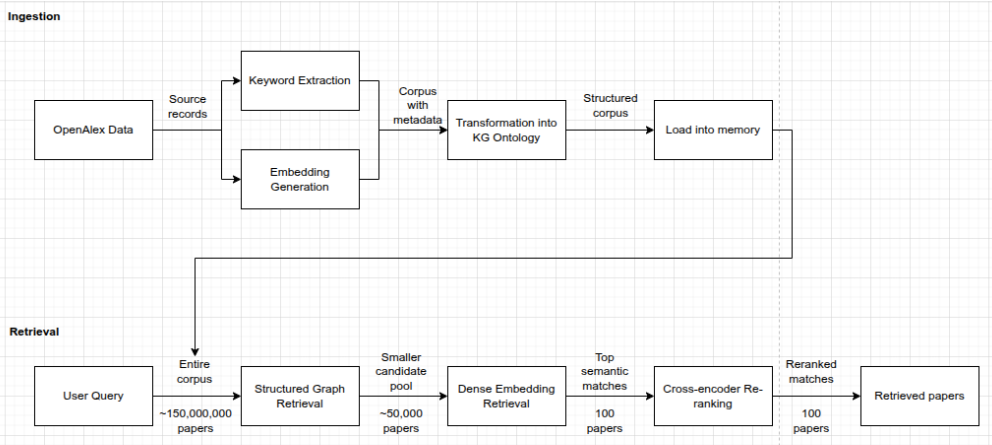
\includegraphics[width=\linewidth]{images/system_architecture.png}
    \caption{System architecture. An ingestion pipeline builds the knowledge graph that a three-stage retrieval cascade queries. The candidate pool size is illustrative and varies by query.}
    \label{fig:system-architecture}
\end{figure}

The system has two parts. An offline ingestion pipeline builds the knowledge graph from source data, and an online retrieval pipeline answers queries against it in three stages. Figure~\ref{fig:system-architecture} shows the overall design.

At a high level, the system uses an ingestion pipeline that:

\begin{itemize}
    \item takes OpenAlex as the source of paper data, namely the title, abstract, authors, and publication date of each work;
    \item extracts the keyphrases and dense embedding of each work from its title and abstract;
    \item transforms the data into the ontology chosen to represent the scholarly domain;
    \item loads the result into the database.
\end{itemize}

OpenAlex was chosen as the source because it is the largest fully open scholarly index and is the successor to the Microsoft Academic Graph, as established in Section~\ref{subsec:kg-infrastructure}. The keyphrases and embeddings extracted in this stage are not incidental products. They are the data that the first and second retrieval stages depend on. How each field is sourced and extracted, and the schema the data is transformed into, are documented in Section~\ref{subsec:component-design}.

For retrieval, the system uses a three-stage pipeline:

\begin{itemize}
    \item Structured graph retrieval, which produces the initial candidate pool. A natural-language query is translated into a structured representation of the keywords to search for and the Boolean logic that combines them, with keywords taken either from the query or from explicit user input. These keywords are matched against the graph's keyword nodes using BM25, and the papers attached to the matched nodes are retrieved and combined under the requested AND, OR, and NOT logic.
    \item Dense embedding retrieval, which narrows the candidate pool by semantic similarity. The query and each candidate paper are represented as high-dimensional vectors, and the candidates closest to the query by cosine similarity are kept, up to the top 100.
    \item Cross-encoder re-ranking, which orders the final results by relevance. A cross-encoder takes the query and a paper's title and abstract together and returns a single relevance score, and the top 100 from the second stage are re-ranked by that score.
\end{itemize}

This extends the two-stage retrieve-then-rerank pattern common to large-scale retrieval systems, placing a knowledge-graph candidate selector in front of the embedding-retrieval and cross-encoder re-ranking stages. Because the three stages increase in both accuracy and cost, each runs over a smaller set than the last, which is necessary because the most accurate stage cannot be run over the full corpus.

Each stage also performs a function the others cannot, which is why all three are present rather than any one alone. The first stage lets the system express typed or structural queries that the other two cannot. As established in Section~\ref{sec:lr-dense}, single-vector dense retrieval cannot represent requests such as papers from a particular author on a given topic published after a given year. Structured retrieval expresses these directly and returns a high-recall candidate set for the later stages to rank. Its output is unbounded. The structured representation and its compilation into a graph query are documented in Section~\ref{subsec:component-design}.

The second stage ranks that candidate set by semantic similarity, which structured retrieval cannot do, since it matches only on shared keywords. Dense embeddings rank candidates by their semantic relatedness to the full query, capturing relevance that exact-term matching misses. Section~\ref{sec:lr-dense} also showed that dense retrieval used alone misses a substantial share of relevant papers and is weak on entity-heavy queries, which is why it ranks a structured candidate set here rather than serving as the primary retrieval mechanism. The embeddings are quantised to reduce their memory footprint, with the quantisation and its justification documented in Section~\ref{subsec:component-design}.

The third stage refines the ranking once more. A bi-encoder compares two vectors that were computed separately, whereas a cross-encoder reads the query and the document together and can weigh their interaction directly, which Section~\ref{sec:lr-dense} identified as the source of the accuracy that late-interaction and cross-encoder approaches achieve over single-vector retrieval. This makes it more accurate but too expensive to run over many papers, which is why it is placed last and applied only to the 100 candidates the earlier stages have selected.

\subsection{Component Design}
\label{subsec:component-design}

\subsubsection{Knowledge Graph Schema}
\label{subsubsec:kg-schema}

\begin{figure}[htbp]
    \centering
    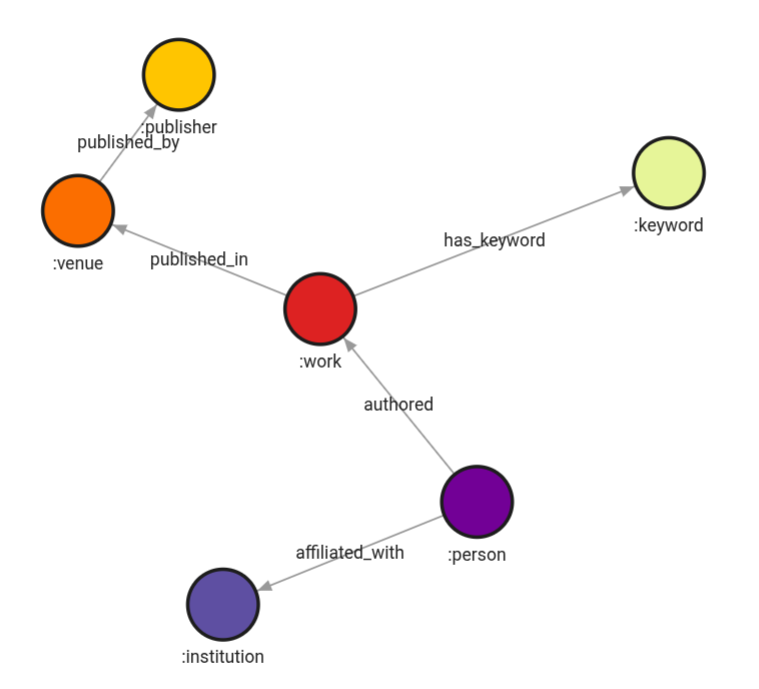
\includegraphics[width=\linewidth]{images/Schema.png}
    \caption{Scholarly Knowledge Graph Schema.}
    \label{fig:kg-schema}
\end{figure}

The schema is general purpose, built from generic entities such as works, keywords, and authors, so that it generalises beyond any single domain despite the biomedical focus of the data it is deployed on.

The design was derived from the knowledge graphs surveyed in Section~\ref{subsec:kg-infrastructure}, which commonly share a similar sub-ontology over the six node types required for retrieval (Work, Person, Institution, Venue, Publisher, and Keyword) and their associated edges. This schema is based on that common structure.

The main point of departure concerns keyword modelling. SemOpenAlex, which is also built on OpenAlex, attaches keywords to the topics assigned to works rather than to the works directly, because OpenAlex derives its keywords at the topic level. Since this schema derives its own keywords per work (Section~\ref{subsubsec:ingestion-storage}), it attaches them directly to the work rather than through a topic node. The resulting schema is shown in Figure~\ref{fig:kg-schema}.

The properties held on each node were refined through internal testing and reduced to the current set, which is given in Appendix~A.

\subsubsection{Ingestion and Storage}
\label{subsubsec:ingestion-storage}

For all purposes excluding benchmarks, the complete OpenAlex snapshot was used as the data source. As established in Section~\ref{subsec:kg-infrastructure}, OpenAlex is the most suitable index due to its large corpus of works and pre-processed metadata.

A biomedical subset was then selected from this snapshot by filtering on the OpenAlex field tag and retaining eleven fields, namely Medicine; Agricultural and Biological Sciences; Biochemistry, Genetics and Molecular Biology; Psychology; Health Profession; Chemistry; Neuroscience; Immunology and Microbiology; Nursing; Pharmacology, Toxicology and Pharmaceutics; and Dentistry. This subset gives the deployed system its biomedical focus, while the schema itself remains general purpose.

For each work in the subset, a keyword generation module and an embedding generation module produce the per-work keywords and the dense embedding that the structured and dense retrieval stages depend on. A number of models for each were benchmarked to inform the selection process, as outlined in Section~\ref{subsec:evaluation-validation}.

The resulting data was transformed to the structure of the ontology, and loaded into Memgraph using their documented best practices. Memgraph was used as an in-memory graph database, on a virtual machine provisioned with sufficient memory to hold the full graph. Memgraph was chosen for the query performance of an in-memory store at this scale, for its MAGE library of graph algorithms, and for a licence compatible with the intended use. Because the graph resides in memory, the dense embeddings are quantised from 32-bit floating point to 8-bit integers to fit within the available memory (see Table~\ref{tab:bienc-deploy} for the resulting footprint).

\subsubsection{Structured Graph Retrieval}
\label{subsubsec:structured-retrieval}

The first retrieval stage turns a natural-language query into a Memgraph-compatible Cypher query through a sequence of learned and deterministic sub-modules.

The query is first normalised, which collapses whitespace, resolves year hints into year bounds, and pulls out quoted phrases as exact-match terms, preserving case so that proper nouns and acronyms survive.

The normalised query is then converted into an Intermediate Representation (IR) using an LLM via a forced tool call whose schema mirrors the representation. The IR couples two components: firstly, a flat list of typed entities, each carrying a type, value, confidence and exact flag; secondly, a recursive boolean expression over those entities using AND, OR and NOT. This design aims to decouple LLM-based intent extraction from deterministic query construction, taking the flexibility of the former whilst keeping the correctness guarantee of the latter, as noted in Section~\ref{sec:lr-nl2q}. The representation is then validated, dropping low-confidence entities and rejecting any query with no entities to anchor the traversal.

The deterministic compiler turns the validated representation into Cypher. Rather than translating the boolean tree into nested graph patterns, it runs one subquery per entity, matching non-exact entities with BM25 over a text index and exact entities by direct property match. It then keeps each work whose matched entities satisfy the boolean expression.

Formally, for each entity $e_{i}$, let $W_{i}$ be the set of works that match it, subject to the work-level filters. Satisfaction of an expression $\varphi$ by a work $w$, written $w \models \varphi$, is defined by recursion over the structure of $\varphi$,
%
\begin{align*}
    w \models e_{i} &\quad\text{iff}\quad w \in W_{i}, \\
    w \models \mathrm{AND}(\varphi_{1}, \ldots, \varphi_{k}) &\quad\text{iff}\quad w \models \varphi_{j} \text{ for every } j, \\
    w \models \mathrm{OR}(\varphi_{1}, \ldots, \varphi_{k}) &\quad\text{iff}\quad w \models \varphi_{j} \text{ for some } j, \\
    w \models \mathrm{NOT}(\varphi) &\quad\text{iff}\quad \lnot\,(w \models \varphi).
\end{align*}
%
The leaves $e_{i}$ are the query's entities and $E$ is its full boolean expression, so the candidate set returned by the stage is
%
\[
    \{\, w \in \bigcup_{i} W_{i} \mid w \models E \,\},
\]
%
where $\bigcup_{i} W_{i}$ is the set of works matching at least one entity. Restricting the universe in this way ensures that a NOT excludes works within the matched set rather than admitting the works that match nothing, and the recursion preserves arbitrary nesting of the operators.

The compiled query runs against the database and returns the candidate pool together with its total match count. A worked example of a query, its intermediate representation, and the compiled Cypher is given in Appendix~B.
% Note: this is what they should look like when compiled.

\subsubsection{Dense Embedding Retrieval and Re-ranking}
\label{subsubsec:dense-rerank}

The second and third stages, dense embedding retrieval and cross-encoder re-ranking, are established techniques rather than novel contributions of this work, and their role within the cascade is described in Section~\ref{subsec:system-architecture}. The retrieve-then-rerank pattern they follow is reviewed in Section~\ref{sec:lr-dense}. The embedding and cross-encoder models are each selected by the benchmarking in Section~\ref{subsec:evaluation-validation}, and the generation and quantisation of the embeddings, together with the memory budget, are covered in Section~\ref{subsubsec:ingestion-storage}.

\subsection{Evaluation and Validation Design}
\label{subsec:evaluation-validation}

\begin{figure}[htbp]
    \centering
    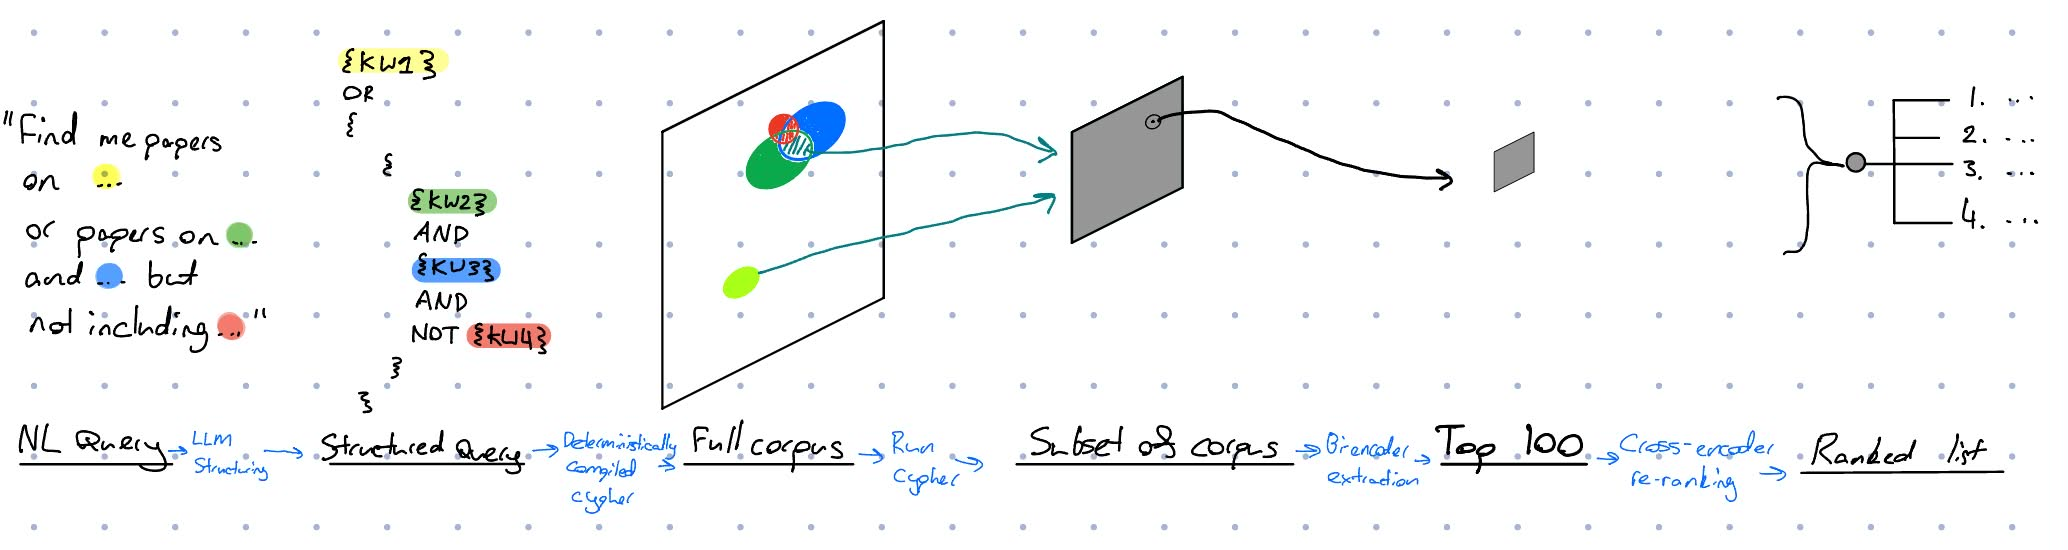
\includegraphics[width=\linewidth]{images/retrieval_pipeline.png}
    \caption{End-to-end representation of pipeline.}
    \label{fig:pipeline}
\end{figure}

\begin{table}[htbp]
    \centering
    \caption{Validation design}
    \label{tab:validation-design}
    \begin{tabularx}{\linewidth}{@{}p{2.4cm}%
        >{\raggedright\arraybackslash}X%
        >{\raggedright\arraybackslash}X%
        >{\raggedright\arraybackslash}X@{}}
        \toprule
        \textbf{Component} & \textbf{Validation Target} & \textbf{Dataset} & \textbf{Metric} \\
        \midrule
        Keyword extraction   & Keyword quality              & KPBiomed, OAGKX, PubMedAKE     & Present/absent F1@5 (stemmed)        \\
        IR extraction        & Query-understanding accuracy & Hand-built stratified gold set & Entity match + logical equivalence   \\
        Dense bi-encoder     & Retrieval quality            & SciRepEval ad-hoc search       & nDCG                                 \\
        Cross-encoder        & Re-ranking quality           & SciRepEval ad-hoc search       & nDCG                                 \\
        Embedding quantisation & Int8 accuracy cost         & SciRepEval ad-hoc search       & nDCG (fp32 vs.\ int8)                \\
        \bottomrule
    \end{tabularx}
\end{table}

Each component designed in Section~\ref{subsec:component-design} is validated independently, against established benchmarks to allow for a comparison of models, from which one can be selected for the final system. This component-wise validation strategy, as summarised in Table~\ref{tab:validation-design}, acts as the counterpart to the design outlined in Section~\ref{subsec:component-design}, following the design and validation approach of Section~\ref{subsec:design-approach}. The outcome of each benchmark, including the model selected, is reported in the Data and Results section.

\subsubsection{Keyword Generation}
\label{subsubsec:keyword-generation}

The keyword generation module of Section~\ref{subsubsec:ingestion-storage} is evaluated against three keyphrase datasets, namely KPBiomed, OAGKX, and PubMedAKE, each of which pairs documents with reference keyphrases. Reference keyphrases are split into present (extractive) keyphrases, which occur verbatim in the source text, and absent (abstractive) keyphrases, which do not and so must be generated. Each is scored by F1@5 with light stemming, so that a keyphrase and its stem count as a match while a different word of the same meaning does not. The present/absent split isolates faithful extraction from generation, which matters because a language-model extractor can hallucinate keyphrases the source does not contain. 

The candidates place a large-language-model generator, GPT-5.4-nano, against established statistical and neural baselines: TF-IDF, YAKE, TextRank, and MultipartiteRank as statistical or graph-based extractors; KeyBERT-MiniLM and KBIR-inspec as neural extractors; and KeyBART as a fine-tuned generative model. The purely extractive baselines can match only present keyphrases by construction, whereas the generative models can also attempt absent ones, so the present/absent split doubles as a comparison between the two families.

\subsubsection{IR Extraction}
\label{subsubsec:ir-extraction}

This benchmark measures how well the model turns an unstructured query into the structured nested boolean representation, the IR (Section~\ref{subsubsec:structured-retrieval}). The model's output is compared against a correct IR written by hand, an approach known as intrinsic evaluation, rather than judging the model by the quality of the final search results. This is done to separate the two possible sources of error. If the system were judged only on its final results, a poor result could come from a mistake in the translation step or in the later search stages, with no way to tell which. Comparing against a correct IR measures the translation step on its own.

The benchmark was built by hand, because the literature (Section~\ref{sec:lr-gap}) found that no existing benchmark covers this task in the scholarly domain. It was constructed as follows:

\begin{itemize}
    \item A set of sample queries was curated to match the vocabulary expected of users, including technical keywords, researcher names, institutions, and venues, so that every entity type the system supports is exercised. The queries span a range of difficulty, from a single topic, through queries that combine topics with AND, OR, and NOT, up to queries that group these with brackets. The simple queries were taken from an existing retrieval dataset, SciRepEval, and the harder ones, which everyday queries rarely contain, were based on the structure of expert queries written for systematic reviews, the exhaustive evidence searches common in fields like medicine.
    \item For each query, the correct nested boolean representation was written by hand. Where a query was ambiguous in how its terms should be grouped, the wording was tightened or brackets were added, so that each query has a single intended answer.
\end{itemize}

Each model is then scored against the hand-written answers on two parts. The first is the entities, the individual terms the model pulled out. These are compared to the correct terms allowing small surface differences, such as a word and its stem, but not accepting a different word of the same meaning, since this stage is meant to capture the terms the user actually wrote rather than paraphrase them. The second is the expression, the way those terms are combined with AND, OR, and NOT. This is judged by logical equivalence, meaning the answer counts as correct if it selects the same papers as the hand-written one, even when written in a different but equivalent form. The same request can be arranged in more than one valid way, for example A AND B is the same as B AND A. Several candidate models are scored this way, with the selected model and the scores reported in the Data and Results section.

\subsubsection{Dense Retrieval}
\label{subsubsec:dense-retrieval}

The dense bi-encoder is evaluated on the ad-hoc search tasks of SciRepEval, namely NFCorpus, TREC-CoVID, and Search, measured by nDCG. SciRepEval is an established benchmark for scientific document retrieval (Section~\ref{sec:lr-bench}), and nDCG is the standard measure of ranking quality, which keeps the stage comparable to prior work. 

The candidates comprise general-purpose embedders (Qwen3-Embedding at 0.6B and 4B, EmbeddingGemma-300M, mxbai-embed-large-v1, BGE-M3, and the hosted text-embedding-3-small) alongside the scientific fine-tuned SPECTER2 in both its base and ad-hoc-query variants. The set contrasts general-purpose against domain-tuned encoders, and self-hostable against paid-API models (text-embedding-3-small being the sole hosted option), the two axes along which the results divide.

\subsubsection{Cross-Encoder Re-ranking}
\label{subsubsec:cross-encoder}

The cross-encoder is evaluated on the same SciRepEval ad-hoc search tasks under the same metric, by re-ranking the retrieved candidates, so the gain it adds can be read directly against the bi-encoder alone. 

Thirteen rerankers are compared: commercial APIs (Cohere Rerank 4.0 in its Pro and Fast tiers); self-hostable neural rerankers (the Qwen3-Reranker at 0.6B and 4B, jina-reranker-v2, and mxbai-rerank-large-v1); a biomedical domain-specific model (MedCPT); and older cross-encoder baselines (the ms-marco-MiniLM and bge-reranker families, and gte-reranker-modernbert-base). This spread lets the results separate model family and recency from raw parameter count, and general-purpose rerankers from the domain-specific one.

\subsubsection{Embedding Quantisation}
\label{subsubsec:embedding-quantisation}

Quantising the embeddings to int8 (Section~\ref{subsubsec:ingestion-storage}) trades precision for memory, so its cost is measured rather than assumed. The bi-encoder evaluation above is repeated with the embeddings held at int8 and compared against the full-precision result, and the resulting difference in nDCG is the accuracy cost attributed to the quantisation.

\subsubsection{System-Level Evaluation}
\label{subsubsec:system-level}

The composed system has no off-the-shelf end-to-end benchmark, which reflects the gap identified in Section~\ref{sec:lr-limitations}. Under the separation of concerns above, however, the system's behaviour follows from its parts. The structured stage returns the papers matching the boolean query, established by the IR and keyword evaluations together with the deterministic compiler, and the dense stages rank those papers, established by their benchmarks. The component results therefore stand as the primary evidence for the system, subject to two limits stated plainly. First, the dense models are benchmarked on a full corpus rather than on the candidate set they rank within the cascade, so their measured quality is a close proxy for their role here rather than a direct measurement of it. Second, the system returns only papers that match the boolean query, so a paper that is relevant but does not match is not retrieved, which is the precision-oriented behaviour the design intends rather than a defect. A system-level evaluation confirms both points directly: the assembled cascade is compared against a retrieval-augmented LLM and Google Scholar over a curated set of realistic queries, assessed qualitatively per query and with light relevance judgments over the returned results. This comparison is the instrument for RQ3; its results appear in Section~\ref{sec:results-system} and its analysis in Section~\ref{subsec:rq3}.

% ============================================================================
%  Data and Results
%  Include from main.tex with:  % ============================================================================
%  Data and Results
%  Include from main.tex with:  % ============================================================================
%  Data and Results
%  Include from main.tex with:  \input{data_and_results}   (or \include{...})
%
%  Requires in the preamble of main.tex:
%      \usepackage{booktabs}
%      \usepackage{graphicx}
%      \usepackage{array}      % only if you later add >{...} column types
%
%  Figures use placeholder paths under figures/ -- replace with your exports.
%  Tables and figures are referenced with \ref so numbering stays dynamic and
%  any table can be moved to an appendix without breaking the prose.
% ============================================================================

\section{Data and Results}

This section reports the result of each component benchmark from the validation design in Section~II-D, taking the components in turn.

% ----------------------------------------------------------------------------
\subsection{Keyword Generation}

\begin{table}[t]
\caption{KPBiomed keyword extraction, present and absent F1@5 with stemming. Models are ordered by present F1, and GPT-5.4-nano is the deployed model.}
\label{tab:kw-kpbiomed}
\centering
\footnotesize
\begin{tabular}{@{}lrr@{}}
\toprule
Model & Present F1@5 & Absent F1@5 \\
\midrule
\textbf{GPT-5.4-nano} & \textbf{30.86} & 1.95 \\
MultipartiteRank & 19.58 & 0.00 \\
TF-IDF & 18.56 & 0.04 \\
KeyBART & 17.40 & \textbf{2.07} \\
YAKE & 16.79 & 0.02 \\
KBIR-inspec & 16.36 & 0.01 \\
KeyBERT-MiniLM & 8.52 & 0.04 \\
TextRank & 5.11 & 0.00 \\
\bottomrule
\end{tabular}
\end{table}

\begin{figure*}[t]
\centering
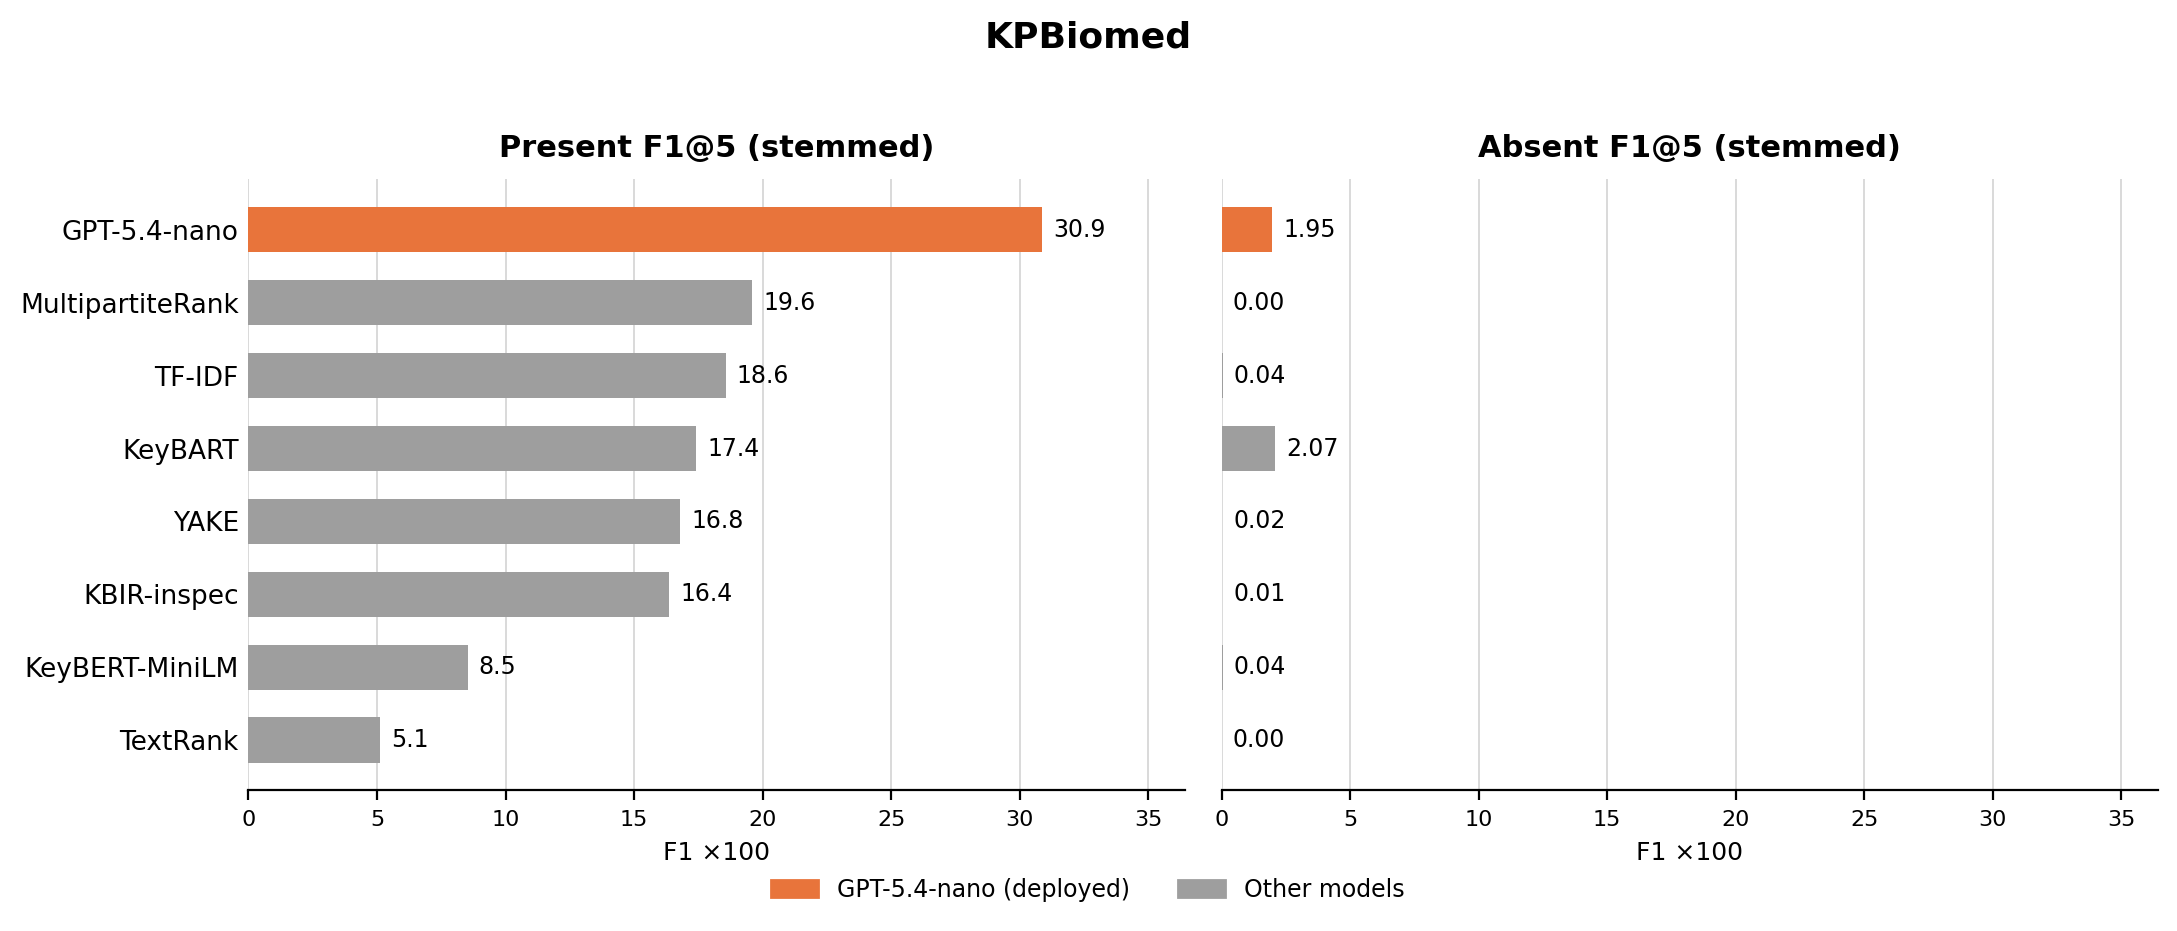
\includegraphics[width=\textwidth]{images/data_and_results/keyword_kpbiomed.png}
\caption{KPBiomed keyword extraction, present and absent F1@5 by model with stemming. The deployed model GPT-5.4-nano is shown in orange and the remaining baselines in grey.}
\label{fig:kw-kpbiomed}
\end{figure*}

\begin{table}[t]
\caption{OAGKX keyword extraction, present and absent F1@5 with stemming. Models are ordered by present F1, and GPT-5.4-nano is the deployed model.}
\label{tab:kw-oagkx}
\centering
\footnotesize
\begin{tabular}{@{}lrr@{}}
\toprule
Model & Present F1@5 & Absent F1@5 \\
\midrule
KeyBART & \textbf{28.42} & \textbf{5.09} \\
\textbf{GPT-5.4-nano} & 26.49 & 1.77 \\
KBIR-inspec & 20.16 & 0.05 \\
MultipartiteRank & 18.83 & 0.00 \\
TF-IDF & 15.55 & 0.03 \\
KeyBERT-MiniLM & 12.04 & 0.04 \\
TextRank & 11.15 & 0.02 \\
YAKE & 8.85 & 0.00 \\
\bottomrule
\end{tabular}
\end{table}

\begin{figure*}[t]
\centering
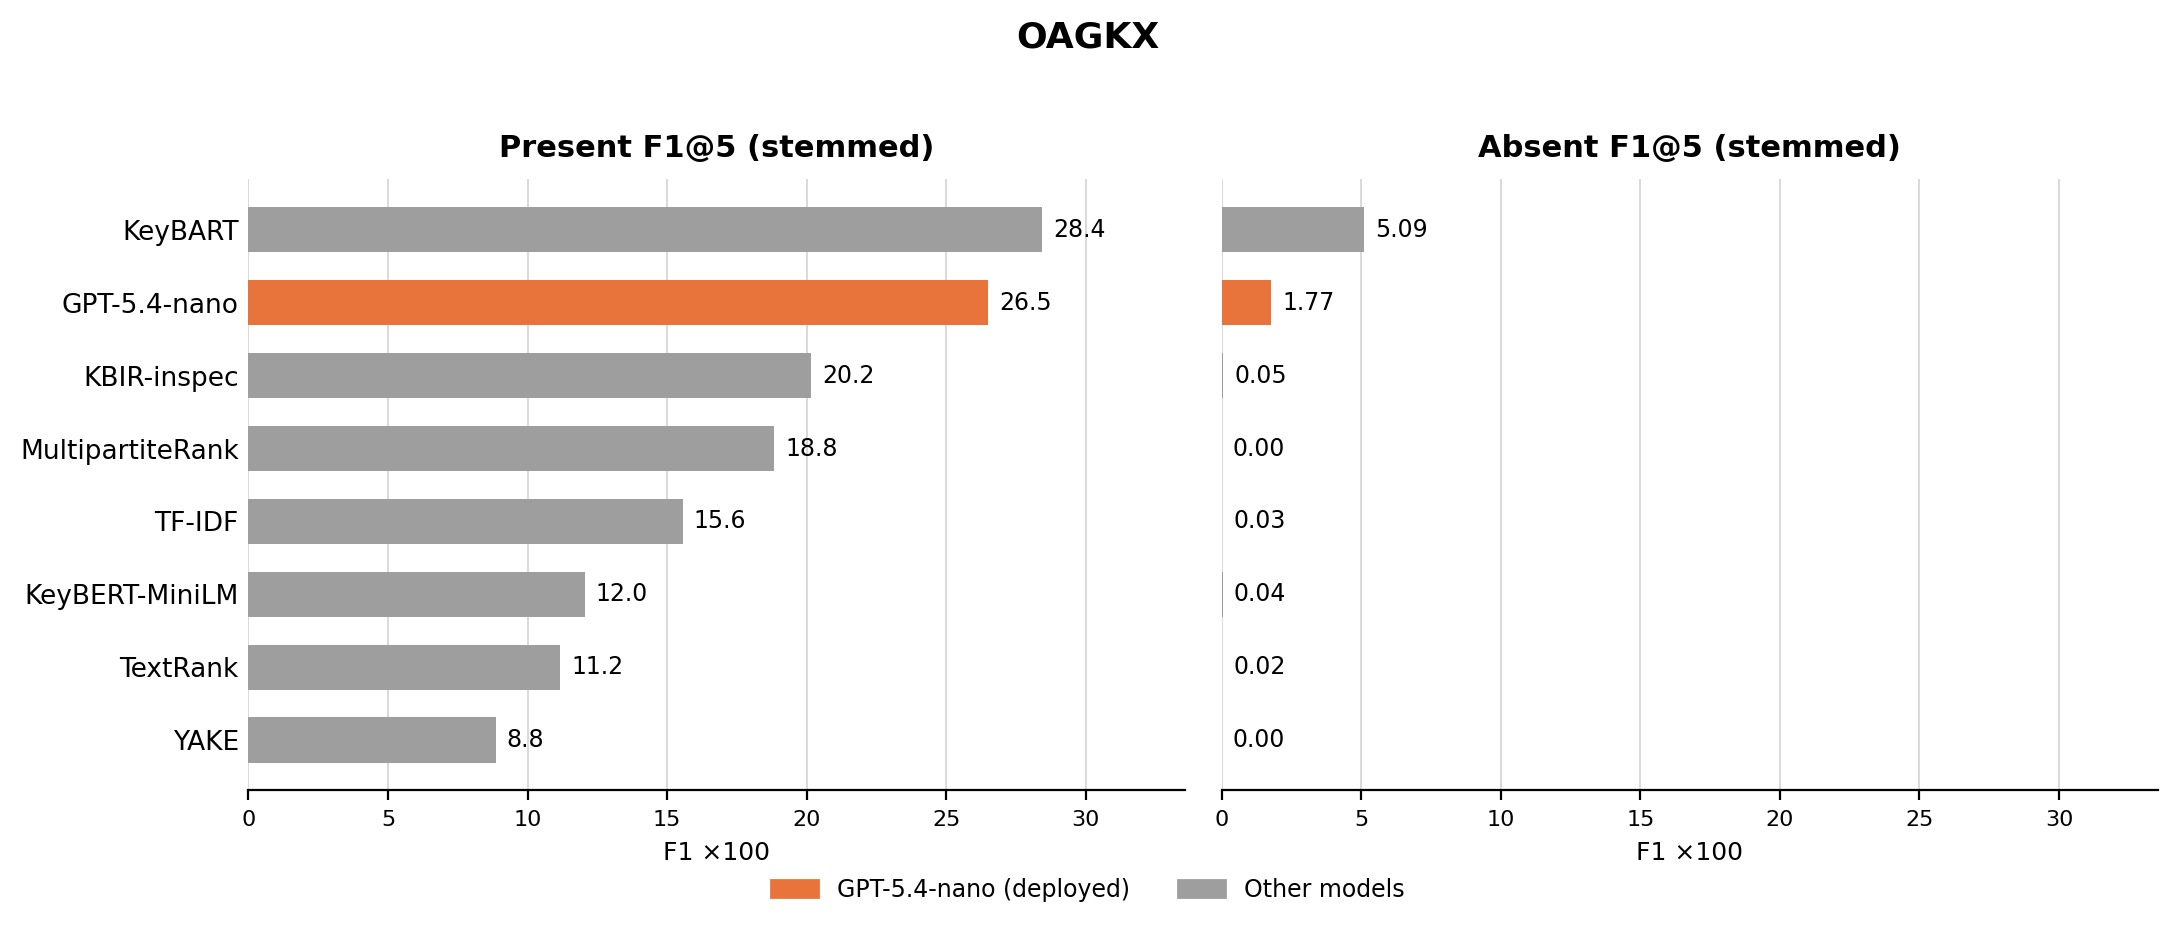
\includegraphics[width=\textwidth]{images/data_and_results/keyword_oagkx.png}
\caption{OAGKX keyword extraction, present and absent F1@5 by model with stemming. The deployed model GPT-5.4-nano is shown in orange and the remaining baselines in grey.}
\label{fig:kw-oagkx}
\end{figure*}

\begin{table}[t]
\caption{PubMedAKE keyword extraction, present and absent F1@5 with stemming. Models are ordered by present F1, and GPT-5.4-nano is the deployed model.}
\label{tab:kw-pubmedake}
\centering
\footnotesize
\begin{tabular}{@{}lrr@{}}
\toprule
Model & Present F1@5 & Absent F1@5 \\
\midrule
\textbf{GPT-5.4-nano} & \textbf{36.44} & \textbf{1.30} \\
TF-IDF & 24.06 & 0.03 \\
MultipartiteRank & 23.06 & 0.00 \\
KBIR-inspec & 19.36 & 0.01 \\
KeyBART & 18.41 & 1.29 \\
YAKE & 12.92 & 0.01 \\
KeyBERT-MiniLM & 6.78 & 0.01 \\
TextRank & 4.68 & 0.00 \\
\bottomrule
\end{tabular}
\end{table}

\begin{figure*}[t]
\centering
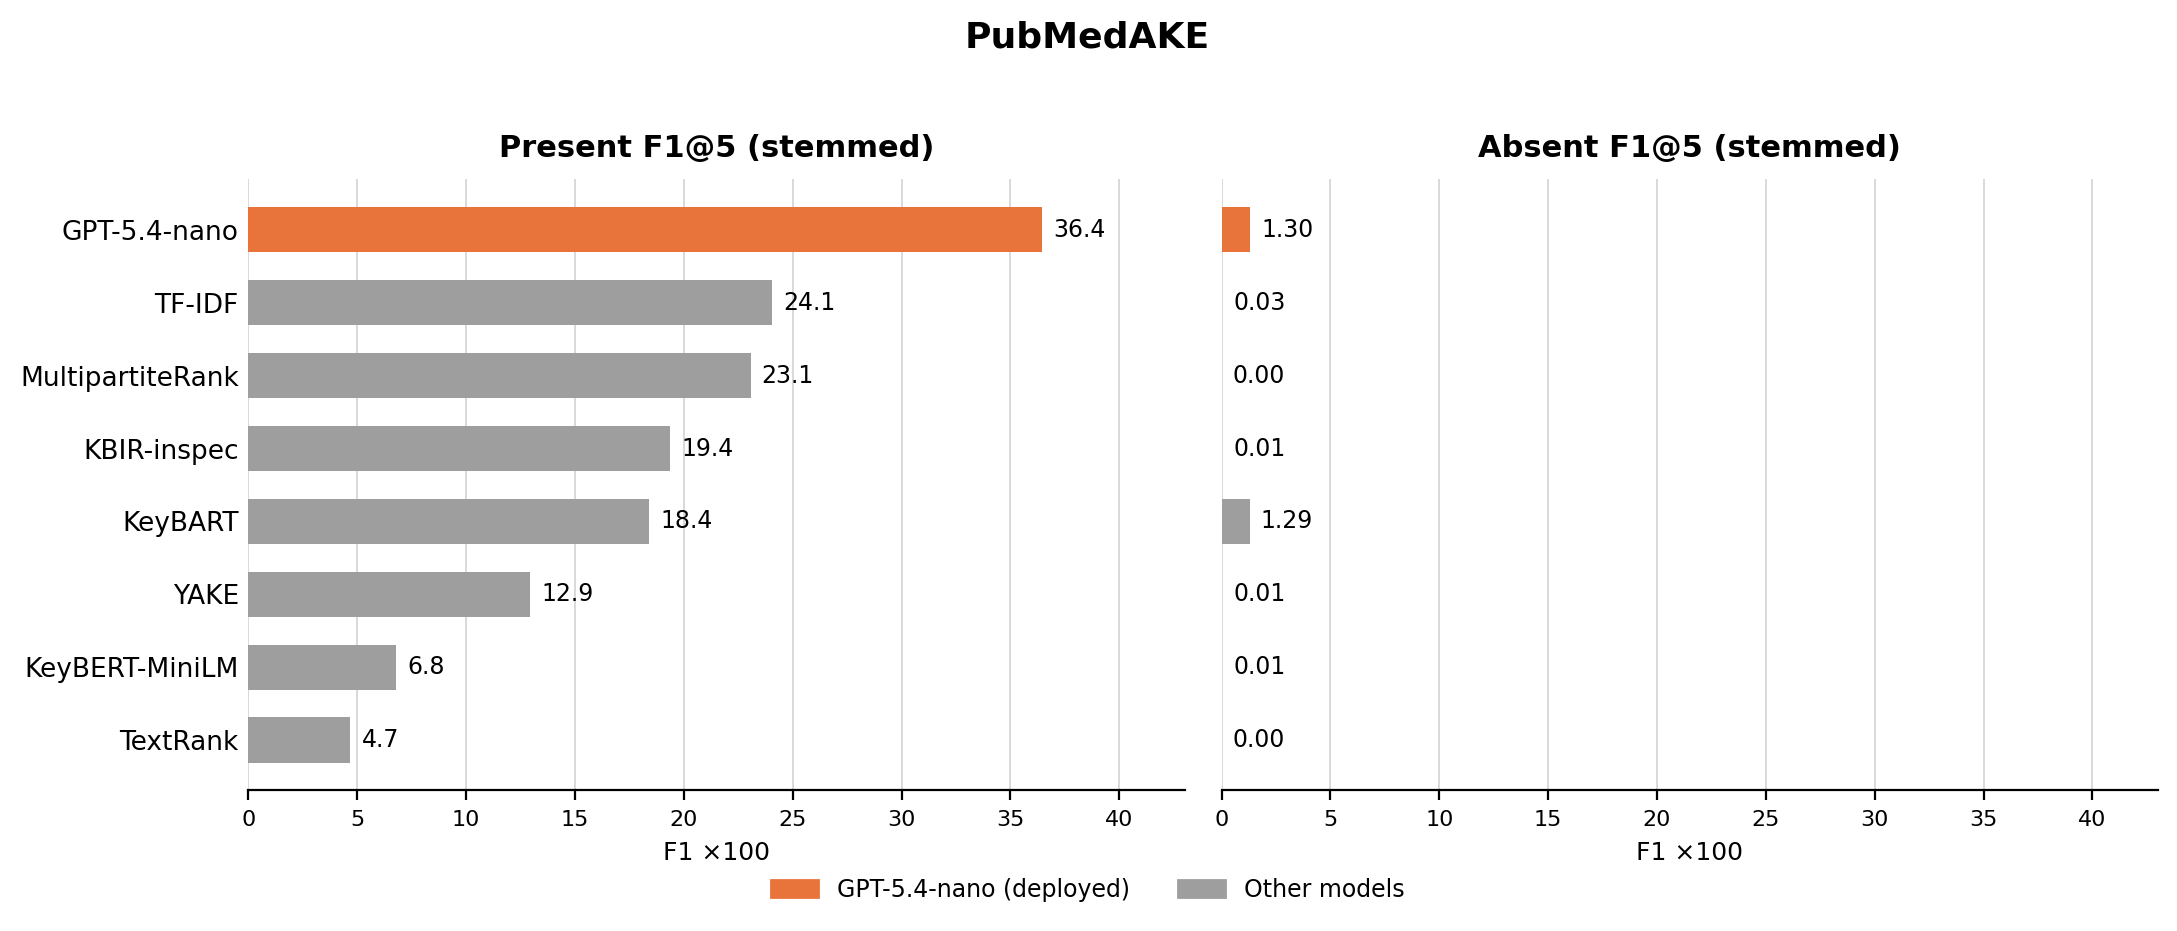
\includegraphics[width=\textwidth]{images/data_and_results/keyword_pubmedake.png}
\caption{PubMedAKE keyword extraction, present and absent F1@5 by model with stemming. The deployed model GPT-5.4-nano is shown in orange and the remaining baselines in grey.}
\label{fig:kw-pubmedake}
\end{figure*}

GPT-5.4-nano was benchmarked for keyword generation against a set of statistical and neural baselines on KPBiomed, OAGKX, and PubMedAKE. Tables~\ref{tab:kw-kpbiomed} to~\ref{tab:kw-pubmedake} report the results for each dataset in turn. Throughout, present (extractive) keyphrases, which occur verbatim in the source text, are distinguished from absent (abstractive) keyphrases, which do not and so must be generated. Matches are scored by F1 at five with light stemming, so that a keyphrase and its stem count as a match while a different word of the same meaning does not.

On the present keyphrase tasks, GPT-5.4-nano records the highest score on KPBiomed and PubMedAKE and the second highest on OAGKX, where KeyBART leads. Its margin is widest on PubMedAKE, at 36.44 against a next-best of 24.06.

On the absent keyphrase tasks, which a model can only score on by producing keyphrases that do not occur in the source text, GPT-5.4-nano scores in the low single digits, from 1.30 on PubMedAKE to 1.95 on KPBiomed. These non-zero scores indicate that the model generates a small portion of its keyphrases rather than extracting all of them. The other generative baseline, KeyBART, behaves similarly and records the highest absent score on KPBiomed and OAGKX. The statistical extractors such as TF-IDF, YAKE, TextRank, and MultipartiteRank remain near zero here, since they return only spans found in the source text and so do not generate at all.

\begin{table}[t]
\caption{Keyword extraction stability for GPT-5.4-nano over three runs on a 2000-document sample.}
\label{tab:kw-stability}
\centering
\footnotesize
\begin{tabular}{@{}p{0.66\columnwidth}r@{}}
\toprule
Quantity & Value \\
\midrule
Set-level Jaccard across runs & 0.73 \\
Present-F1 run-to-run std & $\pm$0.07 \\
Deterministic baselines (TF-IDF, YAKE, TextRank, MultipartiteRank, KeyBERT, KBIR) & 1.00 \\
\bottomrule
\end{tabular}
\end{table}

Table~\ref{tab:kw-stability} reports a reproducibility check for GPT-5.4-nano over three runs on a 2000-document sample. The set-level Jaccard similarity across runs is 0.73, meaning that for a given document around 73 percent of the combined set of keyphrases from any two runs is shared by both, equivalent to roughly one in six keyphrases changing between runs. The model is therefore largely repeatable but not deterministic, unlike the baselines, which are reproducible by construction. The effect on measured performance is negligible, with a run-to-run present-F1 standard deviation of 0.07. The same sample also reproduces the full-split figures to within roughly a tenth of a point, confirming that the smaller stability sample does not shift the headline results.

% ----------------------------------------------------------------------------
\subsection{IR Extraction}

\begin{table*}[t]
\caption{Natural-language-to-IR accuracy by model. Joint IR accuracy counts a query as correct when both its entities and its boolean expression are correct under exact matching, reported in the as-deployed or best configuration for each model.}
\label{tab:ir-accuracy}
\centering
\footnotesize
\begin{tabular}{@{}lllcc@{}}
\toprule
Model & Host & Configuration & IR accuracy & 95\% CI \\
\midrule
\textbf{gpt-5.4-nano} & Azure & default, 0 reasoning tok & \textbf{0.937}$^{\dagger}$ & [0.897, 0.983] \\
gpt-5-mini & Azure & default, 384 reasoning tok & 0.931 & [0.879, 0.974] \\
qwen3:8b & Local (Q4) & single-shot & 0.802 & [0.733, 0.871] \\
qwen3:4b & Local (Q4) & thinking$^{\ddagger}$ & 0.784 & [0.707, 0.862] \\
qwen2.5:3b & Local (Q4) & non-reasoning & 0.207 & [0.138, 0.284] \\
phi4-mini & Local (Q4) & non-reasoning & 0.052 & [0.017, 0.095] \\
llama3.2:3b & Local (Q4) & non-reasoning & 0.026 & [0.000, 0.060] \\
\bottomrule
\end{tabular}

\vspace{3pt}
\begin{minipage}{\linewidth}
\footnotesize\itshape
Confidence intervals are 95 percent bootstrap over 1000 iterations. Cross-model gaps that fall within these intervals are treated as ties, and bold marks the deployed model. The dagger denotes a three-run mean, whose single-run range is 0.914 to 0.940, with temperature zero returning a byte-identical output on 96.6 percent of queries (Table~\ref{tab:ir-stability}). The double dagger denotes qwen3:4b, whose single-shot configuration produced degenerate empty output, so its thinking configuration is its only usable score.
\end{minipage}
\end{table*}

\begin{figure}[t]
\centering
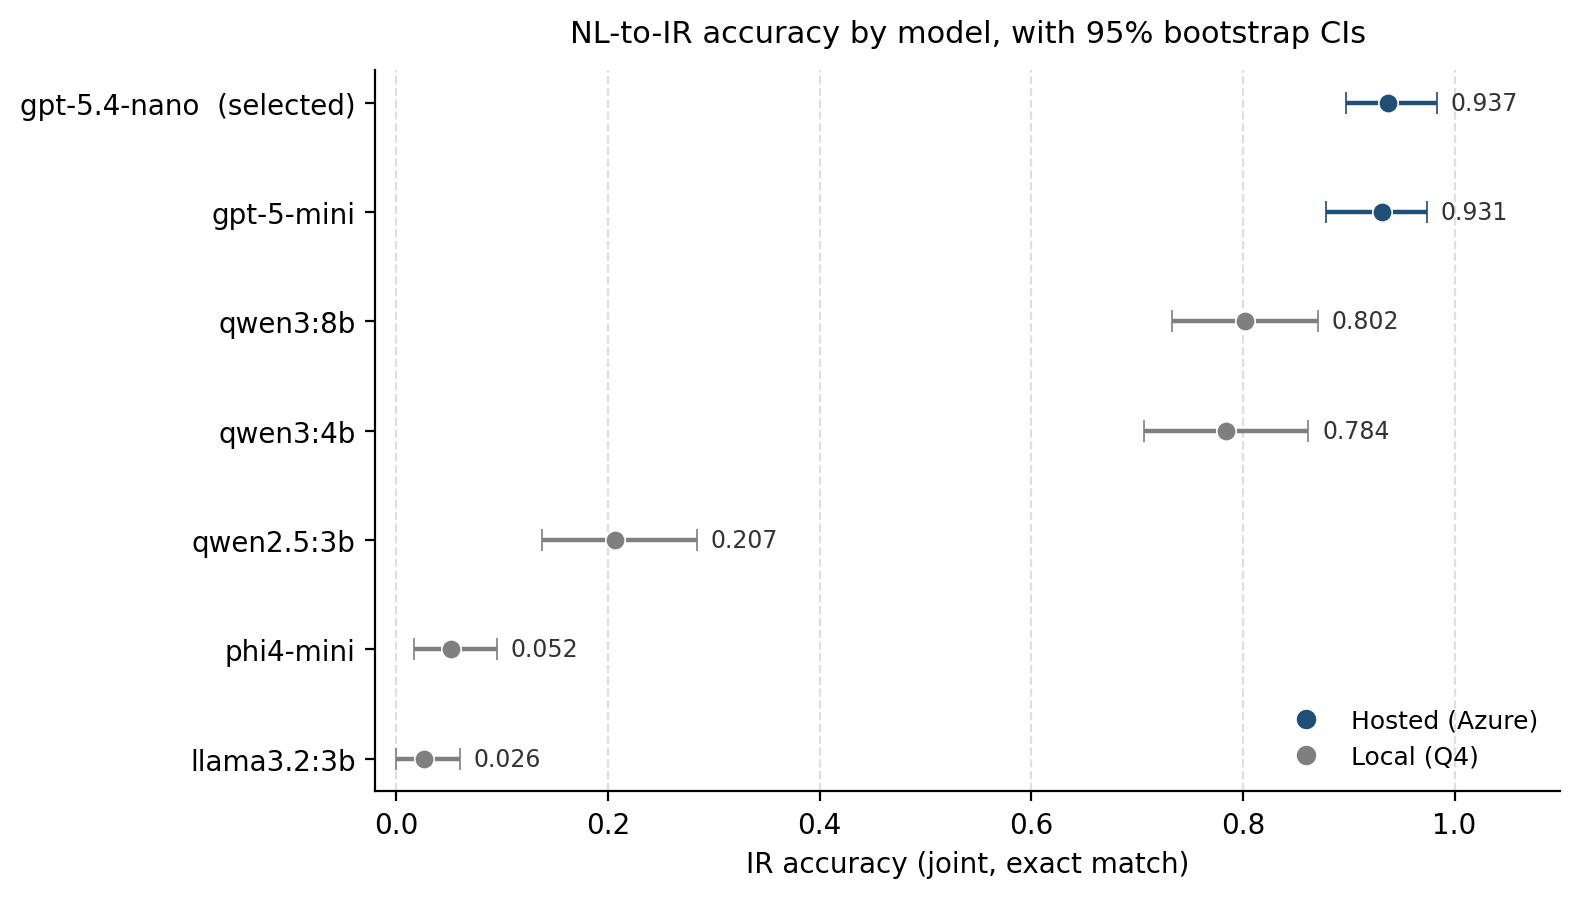
\includegraphics[width=\columnwidth]{images/data_and_results/ir_accuracy_ci.png}
\caption{Natural-language-to-IR joint accuracy by model on the hand-built gold set, with 95 percent bootstrap confidence intervals from 1000 resamples.}
\label{fig:ir-accuracy}
\end{figure}

GPT-5.4-nano was benchmarked for natural-language-to-IR extraction against a set of hosted and local models on a hand-built gold set of queries paired with their correct intermediate representations. The set was constructed to exercise every entity type the system supports across a range of boolean structures, from single topics through to bracketed combinations of AND, OR, and NOT, so that performance on it reflects the input and output behaviour the system actually requires. The headline measure, IR accuracy, is the joint figure reported in Table~\ref{tab:ir-accuracy}, counting a query as correct only when both its extracted entities and its boolean expression are correct under exact matching.

Figure~\ref{fig:ir-accuracy} plots each model's accuracy with its 95 percent bootstrap interval. The two hosted models lead the benchmark by a clear margin, with GPT-5.4-nano highest at an IR accuracy of 0.937 and GPT-5-mini close behind at 0.931. Both hosted intervals clear those of every local model without overlap, placing the hosted advantage beyond sampling noise, while the two overlap each other and are statistically indistinguishable. Among the local models, the two strongest (qwen3:8b and qwen3:4b) reach around 0.80, and the three smaller models fall away sharply to 0.207, 0.052, and 0.026, near the floor of the task.

\begin{table}[t]
\caption{Effect of reasoning on IR accuracy.}
\label{tab:ir-reasoning}
\centering
\footnotesize
\begin{tabular}{@{}lccc@{}}
\toprule
Model & Reasoning off & Reasoning on & $\Delta$ \\
\midrule
gpt-5.4-nano & 0.914 & 0.922 & +0.008 \\
gpt-5-mini & \textbf{0.750} & \textbf{0.940} & \textbf{+0.190} \\
\bottomrule
\end{tabular}

\vspace{3pt}
\begin{minipage}{\linewidth}
\footnotesize\itshape
Reasoning is controlled through the Azure \texttt{reasoning\_effort} setting with tokens accounted. Reasoning on used approximately 246 tokens per query for gpt-5.4-nano and 896 for gpt-5-mini, while reasoning off used none. Reasoning lifts the weaker model in each tier, while the stronger one is already at its ceiling.
\end{minipage}
\end{table}

Table~\ref{tab:ir-reasoning} isolates the effect of reasoning on the two GPT models. GPT-5.4-nano gains almost nothing from it, moving from 0.914 without reasoning to 0.922 with around 246 reasoning tokens, a difference of 0.008, and so reaches its accuracy in a single pass with no reasoning budget. GPT-5-mini behaves differently, scoring only 0.750 without reasoning and rising to 0.940 once reasoning is enabled, at a cost of around 896 reasoning tokens per query. The stronger model is already at its ceiling unaided, whereas the weaker one becomes competitive only by spending a substantial token budget.

\begin{table}[t]
\caption{Deployed model, metric decomposition in the default-effort configuration.}
\label{tab:ir-decomp}
\centering
\footnotesize
\begin{tabular}{@{}lcc@{}}
\toprule
Metric & Value & 95\% CI \\
\midrule
IR accuracy (joint) & 0.937 & [0.897, 0.983] \\
Entity F1 (micro) & 0.984 & [0.969, 0.995] \\
Entity F1 (macro) & 0.982 & [0.967, 0.994] \\
Expression equivalence & 0.931 & [0.888, 0.974] \\
Expression graded & 0.985 & [0.974, 0.995] \\
\bottomrule
\end{tabular}

\vspace{3pt}
\begin{minipage}{\linewidth}
\footnotesize\itshape
Joint accuracy is bounded by expression equivalence, since entity extraction almost never fails on its own.
\end{minipage}
\end{table}

\begin{table}[t]
\caption{Deployed model, accuracy by stratum, ordered hardest first.}
\label{tab:ir-stratum}
\centering
\footnotesize
\begin{tabular}{@{}lrrr@{}}
\toprule
Stratum & $n$ & IR accuracy & failures \\
\midrule
\texttt{filter\_distractor} & 10 & 0.700 & 3 \\
\texttt{multi\_negation} & 10 & 0.800 & 2 \\
\texttt{deep\_nested} & 12 & 0.833 & 2 \\
\texttt{hard\_typing} & 12 & 0.917 & 1 \\
\texttt{single\_concept} & 6 & 1.000 & 0 \\
\texttt{multi\_concept} & 12 & 1.000 & 0 \\
\texttt{exclusion} & 12 & 1.000 & 0 \\
\texttt{nested} & 12 & 1.000 & 0 \\
\texttt{mixed\_entity} & 16 & 1.000 & 0 \\
\texttt{review\_style} & 14 & 1.000 & 0 \\
\bottomrule
\end{tabular}

\vspace{3pt}
\begin{minipage}{\linewidth}
\footnotesize\itshape
The count $n$ is small per stratum, at sixteen or fewer, so the failure counts are a more reliable read than the rate, and the per-stratum 95 percent intervals are wide, for example \texttt{filter\_distractor} at 0.700 is seven of ten.
\end{minipage}
\end{table}

Tables~\ref{tab:ir-decomp} and~\ref{tab:ir-stratum} decompose the chosen model's performance, which is strong across both components and most query types. By component, entity extraction is near-perfect, with a micro F1 of 0.984 and a macro F1 of 0.982, while expression equivalence is lower at 0.931 (a graded variant that credits partially correct expressions reaches 0.985). The joint IR accuracy of 0.937 is therefore bounded by the expression score, since entity extraction almost never fails on its own. By query type, the model is perfect on six of the ten strata, covering single and multiple concepts, exclusions, nesting, mixed entities, and review-style queries. Its errors concentrate in the remaining four. The largest source is \texttt{filter\_distractor}, where three of ten queries fail because the model miscategorises a filter term such as a year or citation bound as a searchable entity. The rest fall on the structurally hardest queries, with two of ten failing on multiple negations, two of twelve on deep nesting, and one of twelve on hard typing. Per-stratum counts are small, at sixteen queries or fewer, so the failure counts are a more reliable read than the rates.

\begin{table}[t]
\caption{Stability of the deployed model over three runs.}
\label{tab:ir-stability}
\centering
\footnotesize
\begin{tabular}{@{}p{0.46\columnwidth}cc@{}}
\toprule
Metric & temp 0 & temp 0.7 \\
\midrule
IR identical across all 3 runs & 0.966 & 0.957 \\
Run-to-run IR-accuracy std & 0.004 & 0.004 \\
Majority-vote@3 vs single run & 0.931 vs 0.940 & 0.940 vs 0.940 \\
\bottomrule
\end{tabular}

\vspace{3pt}
\begin{minipage}{\linewidth}
\footnotesize\itshape
Temperature zero is highly but not perfectly deterministic, and majority voting adds nothing.
\end{minipage}
\end{table}

Table~\ref{tab:ir-stability} reports a stability check over three runs. Although GPT-5.4-nano is not deterministic, at temperature zero it returns an identical IR on 96.6 percent of queries, with a run-to-run accuracy standard deviation of 0.004. Aggregating three runs by majority vote changes nothing, at 0.931 against 0.940 for a single run, so the three-run mean of 0.937 reported in Table~\ref{tab:ir-accuracy} is used throughout.

% ----------------------------------------------------------------------------
\subsection{Dense Bi-encoder Retrieval}

\begin{table*}[t]
\caption{Dense bi-encoder retrieval on SciRepEval ad-hoc search, nDCG $\times$100 with 95 percent bootstrap confidence intervals.}
\label{tab:bienc-results}
\centering
\scriptsize
\setlength{\tabcolsep}{4pt}
\begin{tabular}{@{}p{3.0cm}llll@{}}
\toprule
Model & NFCorpus & TREC-CoVID & Search & Average \\
\midrule
Qwen3-Embedding-4B (int8) & \textbf{80.02 [77.75, 82.17]} & \textbf{94.28 [92.96, 95.43]} & 75.54 [74.93, 76.17] & \textbf{83.28 [82.35, 84.19]} \\
EmbeddingGemma-300M & 79.13 [76.84, 81.29] & 92.45 [90.68, 94.03] & 75.32 [74.66, 75.93] & 82.30 [81.32, 83.31] \\
Qwen3-Embedding-0.6B & 77.94 [75.75, 80.22] & 93.90 [92.52, 95.10] & 75.03 [74.41, 75.65] & 82.29 [81.32, 83.25] \\
text-embedding-3-small (existing) & 78.78 [76.61, 81.05] & 92.38 [90.58, 93.96] & 75.14 [74.52, 75.74] & 82.10 [81.08, 83.05] \\
mxbai-embed-large-v1 & 79.37 [77.19, 81.72] & 91.77 [90.02, 93.25] & 74.92 [74.29, 75.56] & 82.02 [81.06, 82.96] \\
SPECTER2-adhoc-query & 70.46 [68.01, 72.97] & 90.08 [87.84, 92.13] & \textbf{78.22 [77.60, 78.86]} & 79.59 [78.46, 80.71] \\
BGE-M3 & 74.05 [71.72, 76.35] & 89.21 [87.08, 91.16] & 74.82 [74.20, 75.46] & 79.36 [78.29, 80.42] \\
SPECTER2-base (existing) & 72.03 [69.60, 74.54] & 89.46 [86.99, 91.58] & 73.76 [73.12, 74.41] & 78.42 [77.27, 79.58] \\
\bottomrule
\end{tabular}

\vspace{3pt}
\begin{minipage}{\linewidth}
\footnotesize\itshape
The metric is SciRepEval ad-hoc-search full-ranking nDCG over a per-query candidate pool, not BEIR full-corpus nDCG@10. Confidence intervals are 95 percent bootstrap [lo, hi] over 1000 iterations with seed 42, and bold marks the best point estimate per column. On Average the top five models' intervals overlap, a statistical tie, and SPECTER2-adhoc-query's Search lead is the one between-model gap whose interval clears the general models.
\end{minipage}
\end{table*}

\begin{figure}[t]
\centering
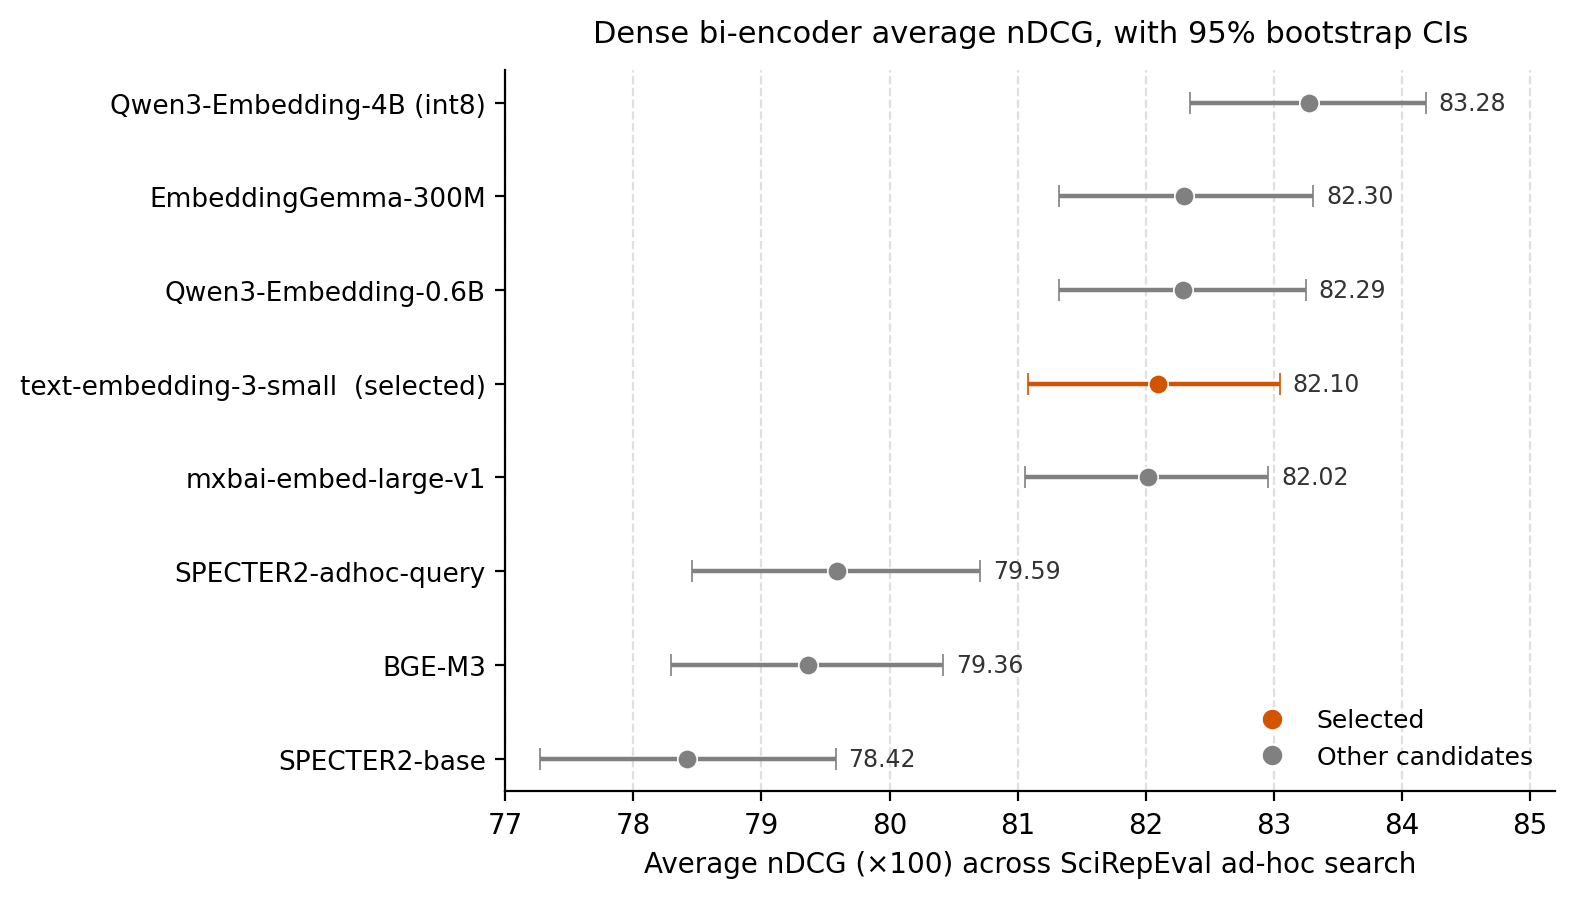
\includegraphics[width=\columnwidth]{images/data_and_results/biencoder_average.png}
\caption{Dense bi-encoder average nDCG across the three SciRepEval ad-hoc search tasks, with 95 percent bootstrap confidence intervals from 1000 resamples. The selected model is shown in orange.}
\label{fig:bienc-avg}
\end{figure}

\begin{figure}[t]
\centering
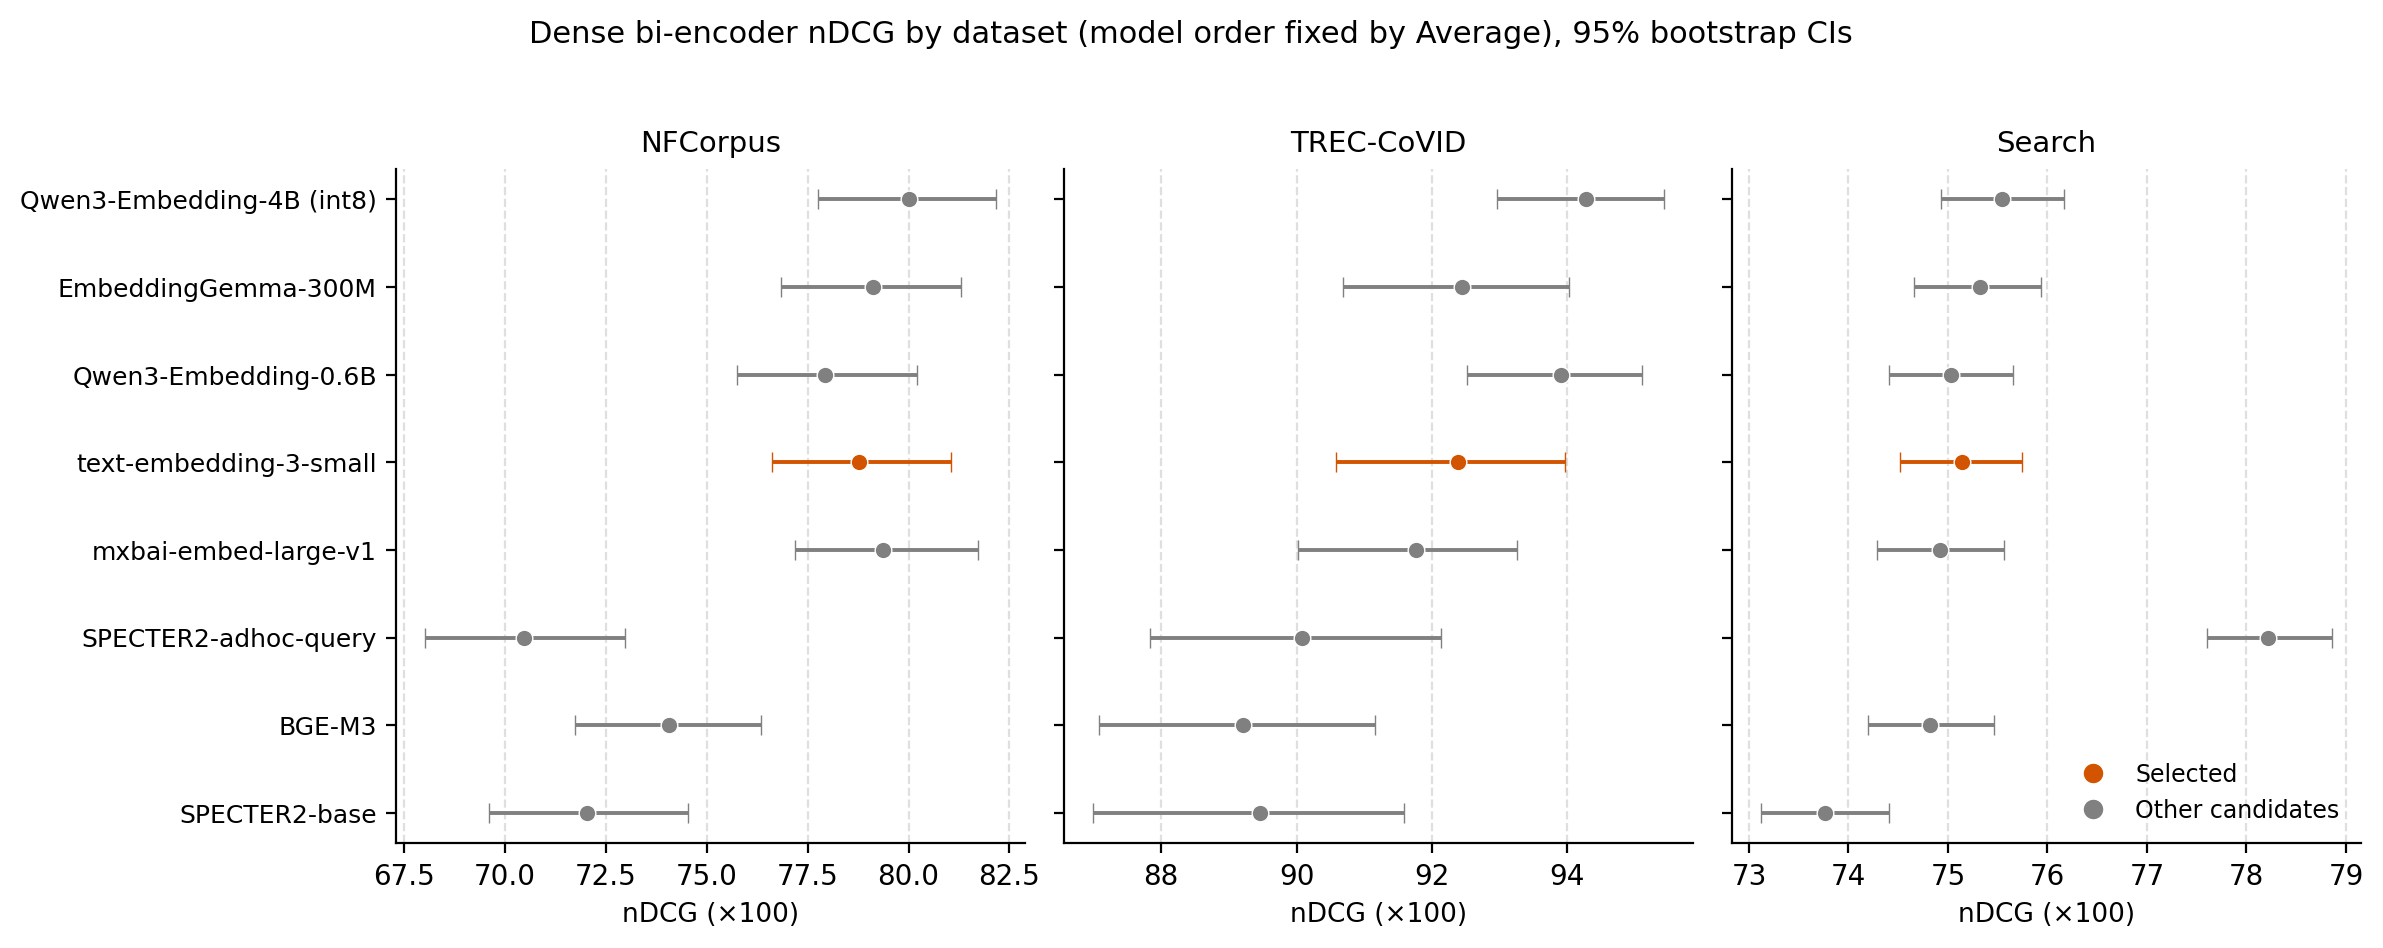
\includegraphics[width=\columnwidth]{images/data_and_results/biencoder_by_dataset.png}
\caption{Dense bi-encoder nDCG on each SciRepEval ad-hoc search task, with models held in their Average order for comparison and 95 percent bootstrap confidence intervals. The selected model is shown in orange.}
\label{fig:bienc-pertask}
\end{figure}

text-embedding-3-small was selected as the dense bi-encoder. The candidate models were evaluated on the three ad-hoc search tasks of SciRepEval, namely NFCorpus, TREC-CoVID, and Search, scored by nDCG. The figure reported is SciRepEval full-ranking nDCG over a per-query candidate pool rather than BEIR full-corpus nDCG@10, which keeps the stage comparable to the scientific retrieval benchmark established in Section~II-D. All scores are nDCG $\times$100 with 95 percent bootstrap intervals from 1000 resamples.

Table~\ref{tab:bienc-results} reports the per-task and average scores in full, and Figure~\ref{fig:bienc-avg} plots each model's average nDCG with its interval. The selected model records an average of 82.10. Qwen3-Embedding-4B holds the highest point estimate at 83.28, but the intervals of the top five models all overlap, forming a statistical tie that contains text-embedding-3-small along with EmbeddingGemma-300M, Qwen3-Embedding-0.6B, and mxbai-embed-large-v1. A clear margin separates this group from the lower three, SPECTER2-adhoc-query at 79.59, BGE-M3 at 79.36, and SPECTER2-base at 78.42, whose intervals fall below the leading cluster.

The average conceals a difference in where each model does its work, shown per task in Figure~\ref{fig:bienc-pertask}. On NFCorpus and TREC-CoVID the general-purpose embedders lead, with Qwen3-Embedding-4B highest on both. On Search the order changes. SPECTER2-adhoc-query scores 78.22 against a field clustered near 75, and this is the single between-model gap on any one task whose interval clears the general models. The same model is weakest on NFCorpus at 70.46, so its Search lead does not survive into the average. The selected model sits within the leading group on each of the three tasks.

\begin{table*}[t]
\caption{Deployment characteristics of the candidate bi-encoders.}
\label{tab:bienc-deploy}
\centering
\footnotesize
\begin{tabular}{@{}lllll@{}}
\toprule
Model & Params (approx.) & Embedding dim & Precision & Self-hostable \\
\midrule
Qwen3-Embedding-4B & $\sim$4 B & 2560 & int8 & yes \\
EmbeddingGemma-300M & $\sim$300 M & 768 & fp16 & yes \\
Qwen3-Embedding-0.6B & $\sim$0.6 B & 1024 & fp16 & yes \\
text-embedding-3-small & undisclosed & 1536 & n/a & no (paid API) \\
mxbai-embed-large-v1 & $\sim$335 M & 1024 & fp16 & yes \\
SPECTER2-adhoc-query & $\sim$110 M & 768 & fp16 & yes \\
BGE-M3 & $\sim$568 M & 1024 & fp16 & yes \\
SPECTER2-base & $\sim$110 M & 768 & fp16 & yes \\
\bottomrule
\end{tabular}

\vspace{3pt}
\begin{minipage}{\linewidth}
\footnotesize\itshape
In-memory footprint per stored vector scales with embedding dimension at int8, at roughly one byte per dimension, giving around 65 GB at 768 dimensions, 87 GB at 1024, 131 GB at 1536, and 218 GB at 2560 over the 85 million works. Encoding cost scales with parameter count.
\end{minipage}
\end{table*}

Table~\ref{tab:bienc-deploy} records the deployment characteristics that the nDCG scores do not, namely approximate parameter count, embedding dimension, precision, and whether the model is self-hostable. In-memory footprint per stored vector scales with embedding dimension at int8, from around 65 GB at 768 dimensions to around 218 GB at 2560 dimensions over the 85 million works, while encoding cost scales with parameter count. The selected model has an embedding dimension of 1536, placing its footprint at around 131 GB, and is served through a paid API rather than self-hosted.

% ----------------------------------------------------------------------------
\subsection{Cross-encoder Re-ranking}

\begin{table*}[t]
\caption{Cross-encoder re-ranking on SciRepEval ad-hoc search, nDCG $\times$100 with 95 percent bootstrap confidence intervals, sorted by Average.}
\label{tab:xenc-results}
\centering
\scriptsize
\setlength{\tabcolsep}{4pt}
\begin{tabular}{@{}p{3.2cm}llll@{}}
\toprule
Model (scorer) & NFCorpus & TREC-CoVID & Search & Average \\
\midrule
Cohere Rerank 4.0 Pro (API) & \textbf{80.42 [78.17, 82.60]} & \textbf{94.60 [93.30, 95.71]} & 75.39 [74.76, 76.00] & \textbf{83.47 [82.54, 84.33]} \\
Qwen3-Reranker-4B (int8) & 80.10 [77.94, 82.14] & 94.37 [92.90, 95.60] & 74.93 [74.32, 75.56] & 83.13 [82.18, 83.99] \\
Cohere Rerank 4.0 Fast (API) & 78.77 [76.55, 80.98] & 94.15 [92.83, 95.31] & \textbf{75.42 [74.75, 76.04]} & 82.78 [81.83, 83.68] \\
Qwen3-Reranker-0.6B (fp16) & 78.06 [75.65, 80.24] & 93.98 [92.59, 95.20] & 75.25 [74.59, 75.85] & 82.43 [81.50, 83.34] \\
mxbai-rerank-large-v1 (435M) & 78.32 [76.08, 80.76] & 91.50 [89.43, 93.33] & 74.78 [74.15, 75.46] & 81.53 [80.48, 82.59] \\
jina-reranker-v2-base (278M) & 76.73 [74.49, 79.01] & 91.84 [90.05, 93.52] & 75.37 [74.73, 75.99] & 81.31 [80.28, 82.30] \\
MedCPT-Cross-Encoder (109M, biomed) & 75.70 [73.21, 78.03] & 88.91 [86.61, 90.97] & 73.97 [73.34, 74.63] & 79.53 [78.40, 80.66] \\
ms-marco-MiniLM-L-6-v2 (22M) & 73.10 [70.78, 75.48] & 88.78 [86.41, 90.90] & 75.21 [74.58, 75.84] & 79.03 [77.90, 80.13] \\
bge-reranker-v2-m3 (568M) & 70.71 [68.31, 73.07] & 90.30 [88.29, 92.18] & 74.40 [73.78, 75.05] & 78.47 [77.37, 79.53] \\
ms-marco-MiniLM-L-12-v2 (33M) & 69.88 [67.41, 72.38] & 87.17 [84.73, 89.52] & 75.09 [74.44, 75.71] & 77.38 [76.17, 78.54] \\
bge-reranker-large (560M) & 66.49 [64.11, 68.85] & 87.27 [84.61, 89.62] & 74.22 [73.59, 74.85] & 76.00 [74.80, 77.16] \\
bge-reranker-base (278M) & 58.75 [56.38, 60.94] & 84.98 [82.12, 87.60] & 72.60 [71.97, 73.24] & 72.11 [70.84, 73.35] \\
gte-reranker-modernbert-base (150M) & 48.88 [46.82, 50.93] & 79.03 [76.40, 81.60] & 69.94 [69.26, 70.60] & 65.95 [64.91, 67.07] \\
\bottomrule
\end{tabular}

\vspace{3pt}
\begin{minipage}{\linewidth}
\footnotesize\itshape
The metric is SciRepEval ad-hoc-search full-ranking nDCG over a reranking pool, not BEIR full-corpus nDCG@10. Confidence intervals are 95 percent bootstrap [2.5 percent, 97.5 percent] over 1000 iterations with seed 42, with the Average resampled independently within each dataset. The intervals are tight on Search, which has 2585 queries, and wide on TREC-CoVID, which has 50, and bold marks the best point estimate per column. The top four models, namely Cohere Pro, Qwen3-Reranker-4B, Cohere Fast, and Qwen3-Reranker-0.6B, have heavily overlapping Average intervals and form a statistical tie, within which the best self-hostable model, Qwen3-Reranker-4B at int8, is tied with Cohere Pro. On Search the small candidate pool saturates every reranker at around 75. For reference, the bi-encoder embeddings without intervals give the best embedder Qwen3-Embedding-4B at 83.28 Average, SPECTER2-adhoc-query at 78.22 on Search, which is above every reranker here, and text-embedding-3-small at 82.10 Average.
\end{minipage}
\end{table*}

\begin{figure}[t]
\centering
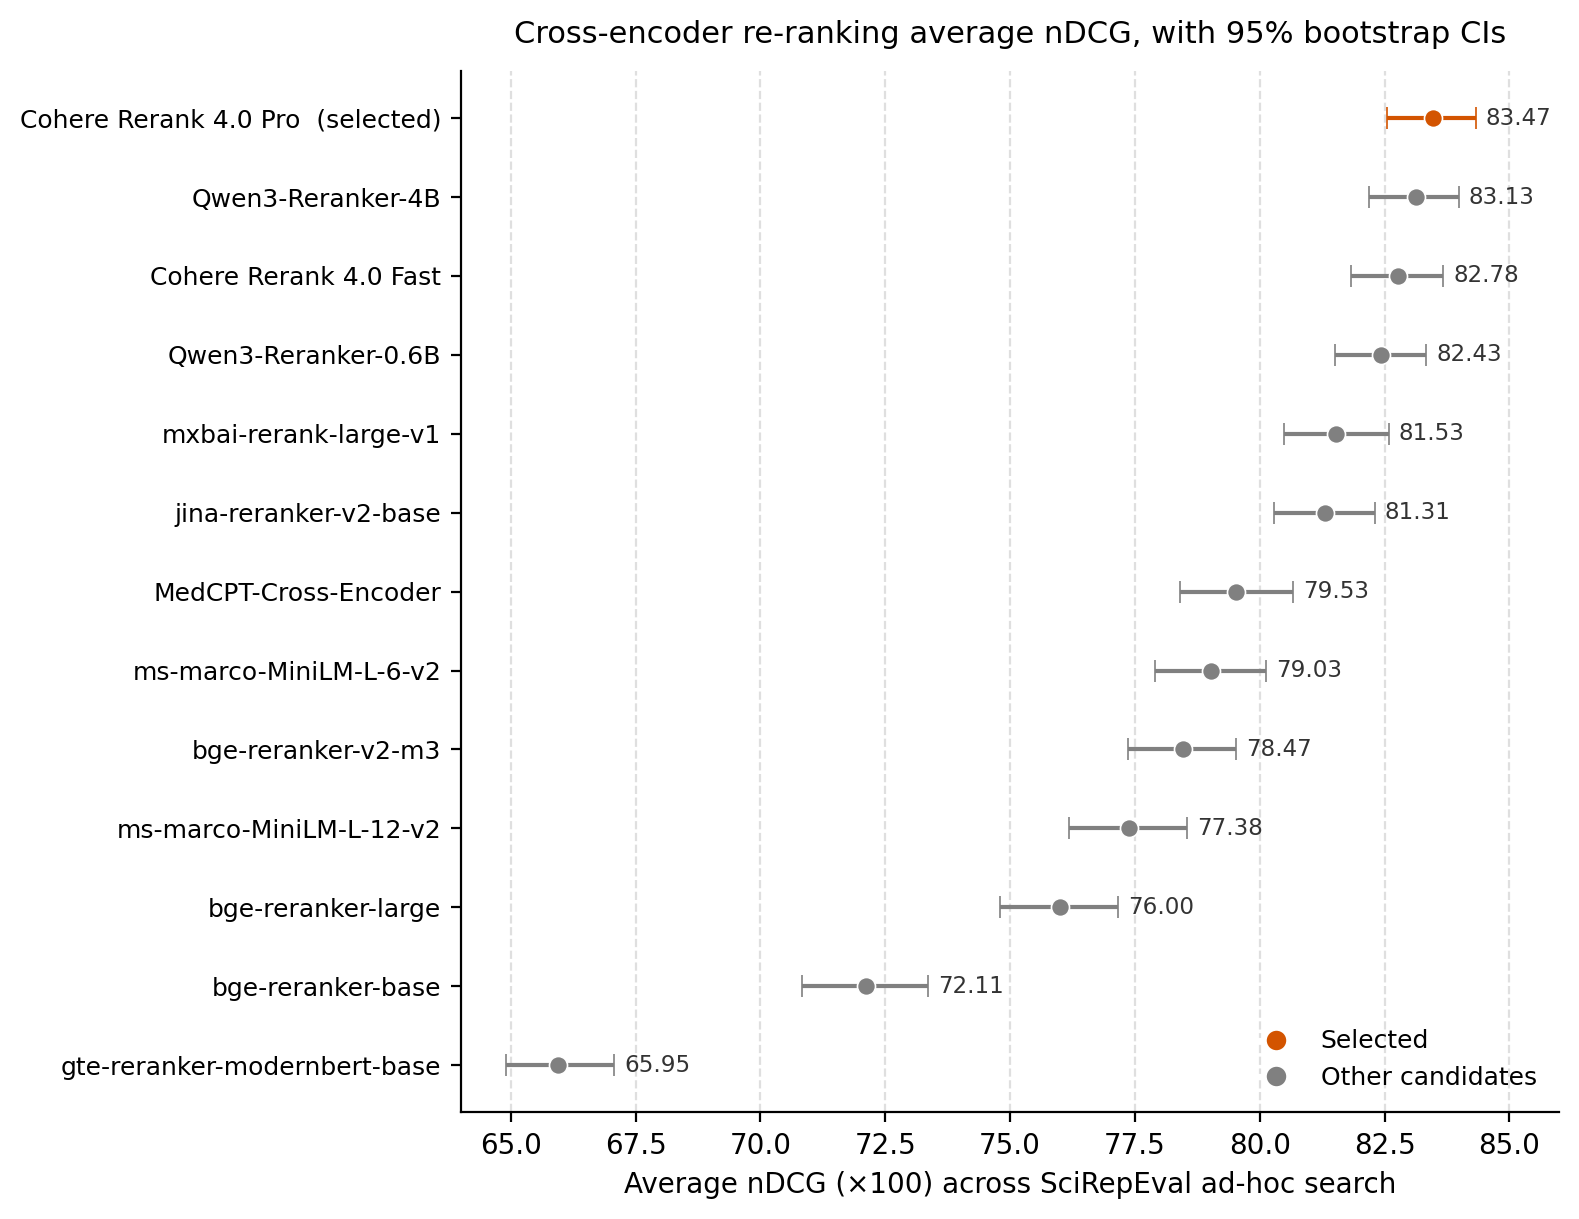
\includegraphics[width=\columnwidth]{images/data_and_results/crossencoder_average.png}
\caption{Cross-encoder re-ranking average nDCG across the three SciRepEval ad-hoc search tasks, with 95 percent bootstrap confidence intervals from 1000 resamples. The selected model is shown in orange.}
\label{fig:xenc-avg}
\end{figure}

\begin{figure}[t]
\centering
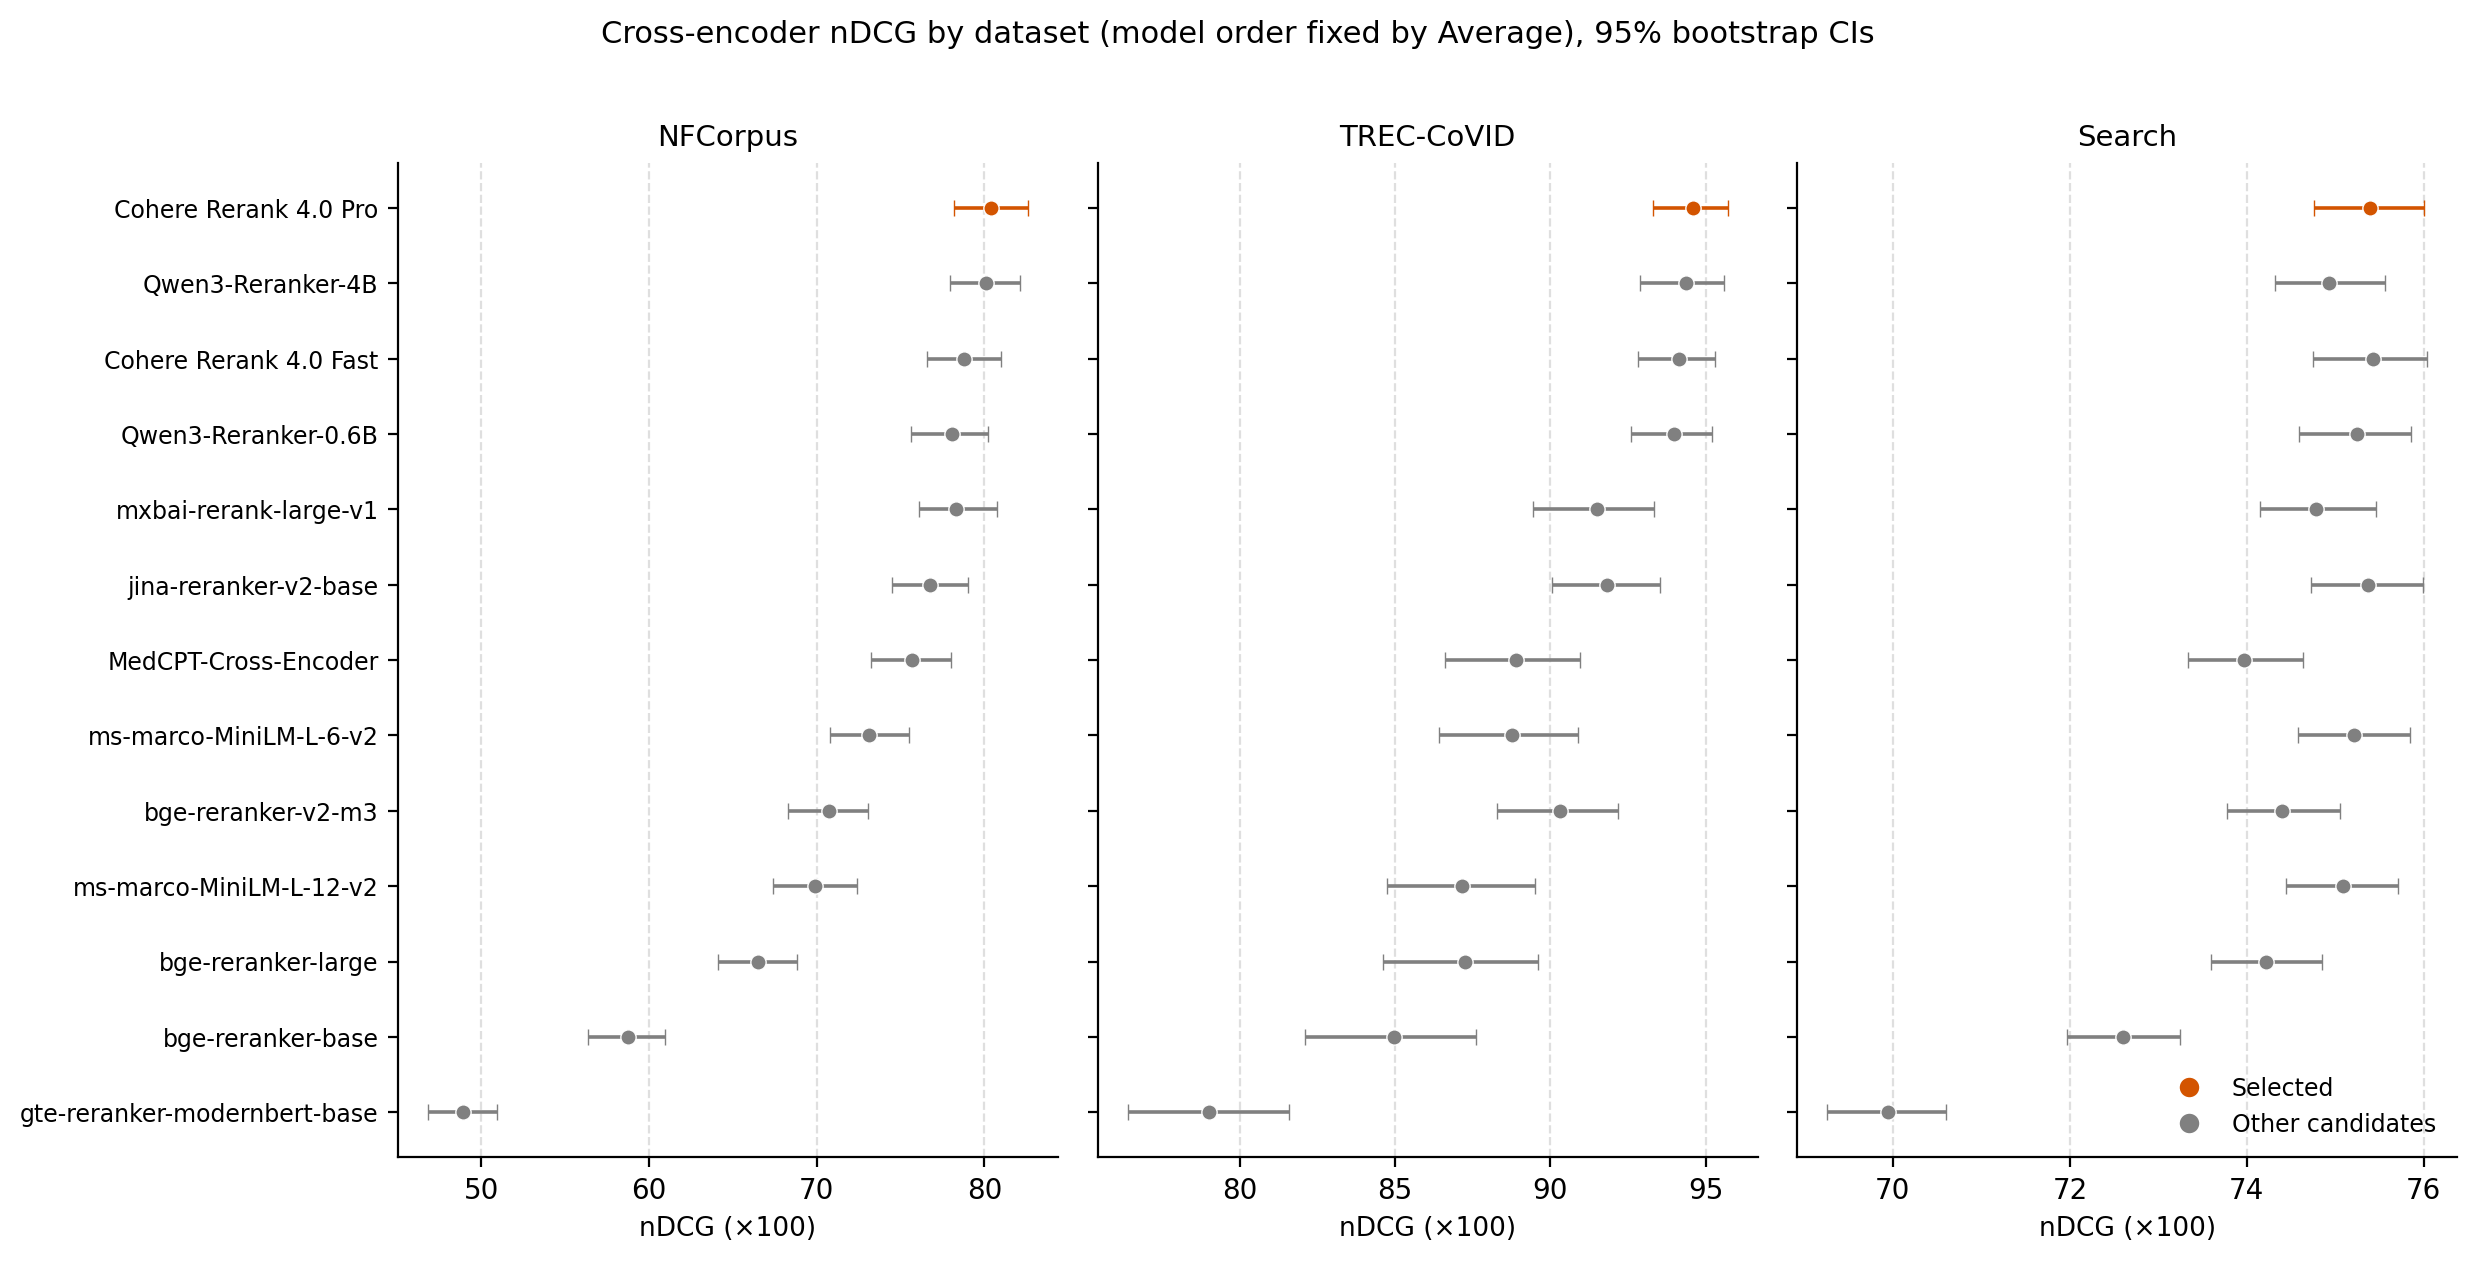
\includegraphics[width=\columnwidth]{images/data_and_results/crossencoder_by_dataset.png}
\caption{Cross-encoder nDCG on each SciRepEval ad-hoc search task, with models held in their Average order for comparison and 95 percent bootstrap confidence intervals. The selected model is shown in orange.}
\label{fig:xenc-pertask}
\end{figure}

Cohere Rerank 4.0 Pro was selected as the cross-encoder. The candidate rerankers were evaluated on the same three SciRepEval ad-hoc search tasks as the bi-encoder and under the same nDCG metric, scoring each model by the ranking it produces when it re-ranks the retrieved candidate pool. All scores are nDCG $\times$100 with 95 percent bootstrap intervals from 1000 resamples. The intervals are tight on Search, which has 2585 queries, and wide on TREC-CoVID, which has 50.

Table~\ref{tab:xenc-results} reports the full per-task and average scores, and Figure~\ref{fig:xenc-avg} plots each model's average with its interval. The selected model holds the highest average at 83.47. Its interval overlaps those of the next three models, Qwen3-Reranker-4B at 83.13, Cohere Rerank 4.0 Fast at 82.78, and Qwen3-Reranker-0.6B at 82.43, so these four form a statistical tie at the top. Within that group the strongest self-hostable model, Qwen3-Reranker-4B, is tied with the selected model. Below the leading four the field descends steadily through a long tail to gte-reranker-modernbert-base at 65.95, a spread of more than seventeen points from top to bottom.

The per-task view in Figure~\ref{fig:xenc-pertask} shows that almost all of this separation comes from NFCorpus, where the models spread across more than thirty points, from 80.42 at the top down to 48.88. Search behaves in the opposite way. Every reranker scores close to 75, since the small candidate pool the stage re-ranks leaves little room to reorder, so the task barely separates the models. TREC-CoVID falls between the two, with a high but noisy spread that reflects its fifty queries.

\begin{table*}[t]
\caption{Deployment characteristics of the candidate cross-encoders.}
\label{tab:xenc-deploy}
\centering
\footnotesize
\begin{tabular}{@{}p{4.5cm}llp{4.0cm}@{}}
\toprule
Model & Params (approx.) & Precision & Self-hostable \\
\midrule
Cohere Rerank 4.0 Pro & undisclosed & n/a & no (paid API) \\
Qwen3-Reranker-4B & $\sim$4 B & int8 & yes (Apache-2.0) \\
Cohere Rerank 4.0 Fast & undisclosed & n/a & no (paid API) \\
Qwen3-Reranker-0.6B & $\sim$0.6 B & fp16 & yes (Apache-2.0) \\
mxbai-rerank-large-v1 & $\sim$435 M & fp16 & yes \\
jina-reranker-v2-base & $\sim$278 M & fp16 & weights CC-BY-NC (non-commercial) \\
MedCPT-Cross-Encoder & $\sim$109 M & fp16 & yes \\
ms-marco-MiniLM-L-6-v2 & $\sim$22 M & fp16 & yes \\
bge-reranker-v2-m3 & $\sim$568 M & fp16 & yes \\
ms-marco-MiniLM-L-12-v2 & $\sim$33 M & fp16 & yes \\
bge-reranker-large & $\sim$560 M & fp16 & yes \\
bge-reranker-base & $\sim$278 M & fp16 & yes \\
gte-reranker-modernbert-base & $\sim$150 M & fp16 & yes \\
\bottomrule
\end{tabular}

\vspace{3pt}
\begin{minipage}{\linewidth}
\footnotesize\itshape
Unlike the bi-encoder, a reranker stores no vectors, so its cost is latency, which scales with parameter count, rather than memory, which is why the stage runs over only around 100 candidates. The Qwen3 rerankers are released under Apache-2.0, while the jina-reranker-v2 weights are CC-BY-NC-4.0 and so are non-commercial and not deployable in a commercial product. The remaining licences should be confirmed against the deployment terms before selection.
\end{minipage}
\end{table*}

Table~\ref{tab:xenc-deploy} records the deployment characteristics, namely approximate parameter count, precision, and whether the model is self-hostable along with its licence. Unlike the bi-encoder, a reranker stores no vectors, so its cost is latency rather than memory and scales with parameter count, which is the reason the stage runs over only around 100 candidates. The self-hostable options carry mixed licences, with the Qwen3 rerankers released under Apache-2.0 and the jina reranker under a non-commercial CC-BY-NC licence, while the selected model is served through a paid API.

% ----------------------------------------------------------------------------
\subsection{Embedding Quantisation}
% Placeholder. Results not yet available.
\textit{[Placeholder. Results comparing int8 against full-precision nDCG, and the resulting accuracy cost, to be added.]}

% ----------------------------------------------------------------------------
\subsection{System-Level Evaluation}
% Placeholder. Results not yet available.
\textit{[Placeholder. End-to-end results over a realistic query set with light relevance judgments to be added.]}   (or \include{...})
%
%  Requires in the preamble of main.tex:
%      \usepackage{booktabs}
%      \usepackage{graphicx}
%      \usepackage{array}      % only if you later add >{...} column types
%
%  Figures use placeholder paths under figures/ -- replace with your exports.
%  Tables and figures are referenced with \ref so numbering stays dynamic and
%  any table can be moved to an appendix without breaking the prose.
% ============================================================================

\section{Data and Results}

This section reports the result of each component benchmark from the validation design in Section~II-D, taking the components in turn.

% ----------------------------------------------------------------------------
\subsection{Keyword Generation}

\begin{table}[t]
\caption{KPBiomed keyword extraction, present and absent F1@5 with stemming. Models are ordered by present F1, and GPT-5.4-nano is the deployed model.}
\label{tab:kw-kpbiomed}
\centering
\footnotesize
\begin{tabular}{@{}lrr@{}}
\toprule
Model & Present F1@5 & Absent F1@5 \\
\midrule
\textbf{GPT-5.4-nano} & \textbf{30.86} & 1.95 \\
MultipartiteRank & 19.58 & 0.00 \\
TF-IDF & 18.56 & 0.04 \\
KeyBART & 17.40 & \textbf{2.07} \\
YAKE & 16.79 & 0.02 \\
KBIR-inspec & 16.36 & 0.01 \\
KeyBERT-MiniLM & 8.52 & 0.04 \\
TextRank & 5.11 & 0.00 \\
\bottomrule
\end{tabular}
\end{table}

\begin{figure*}[t]
\centering
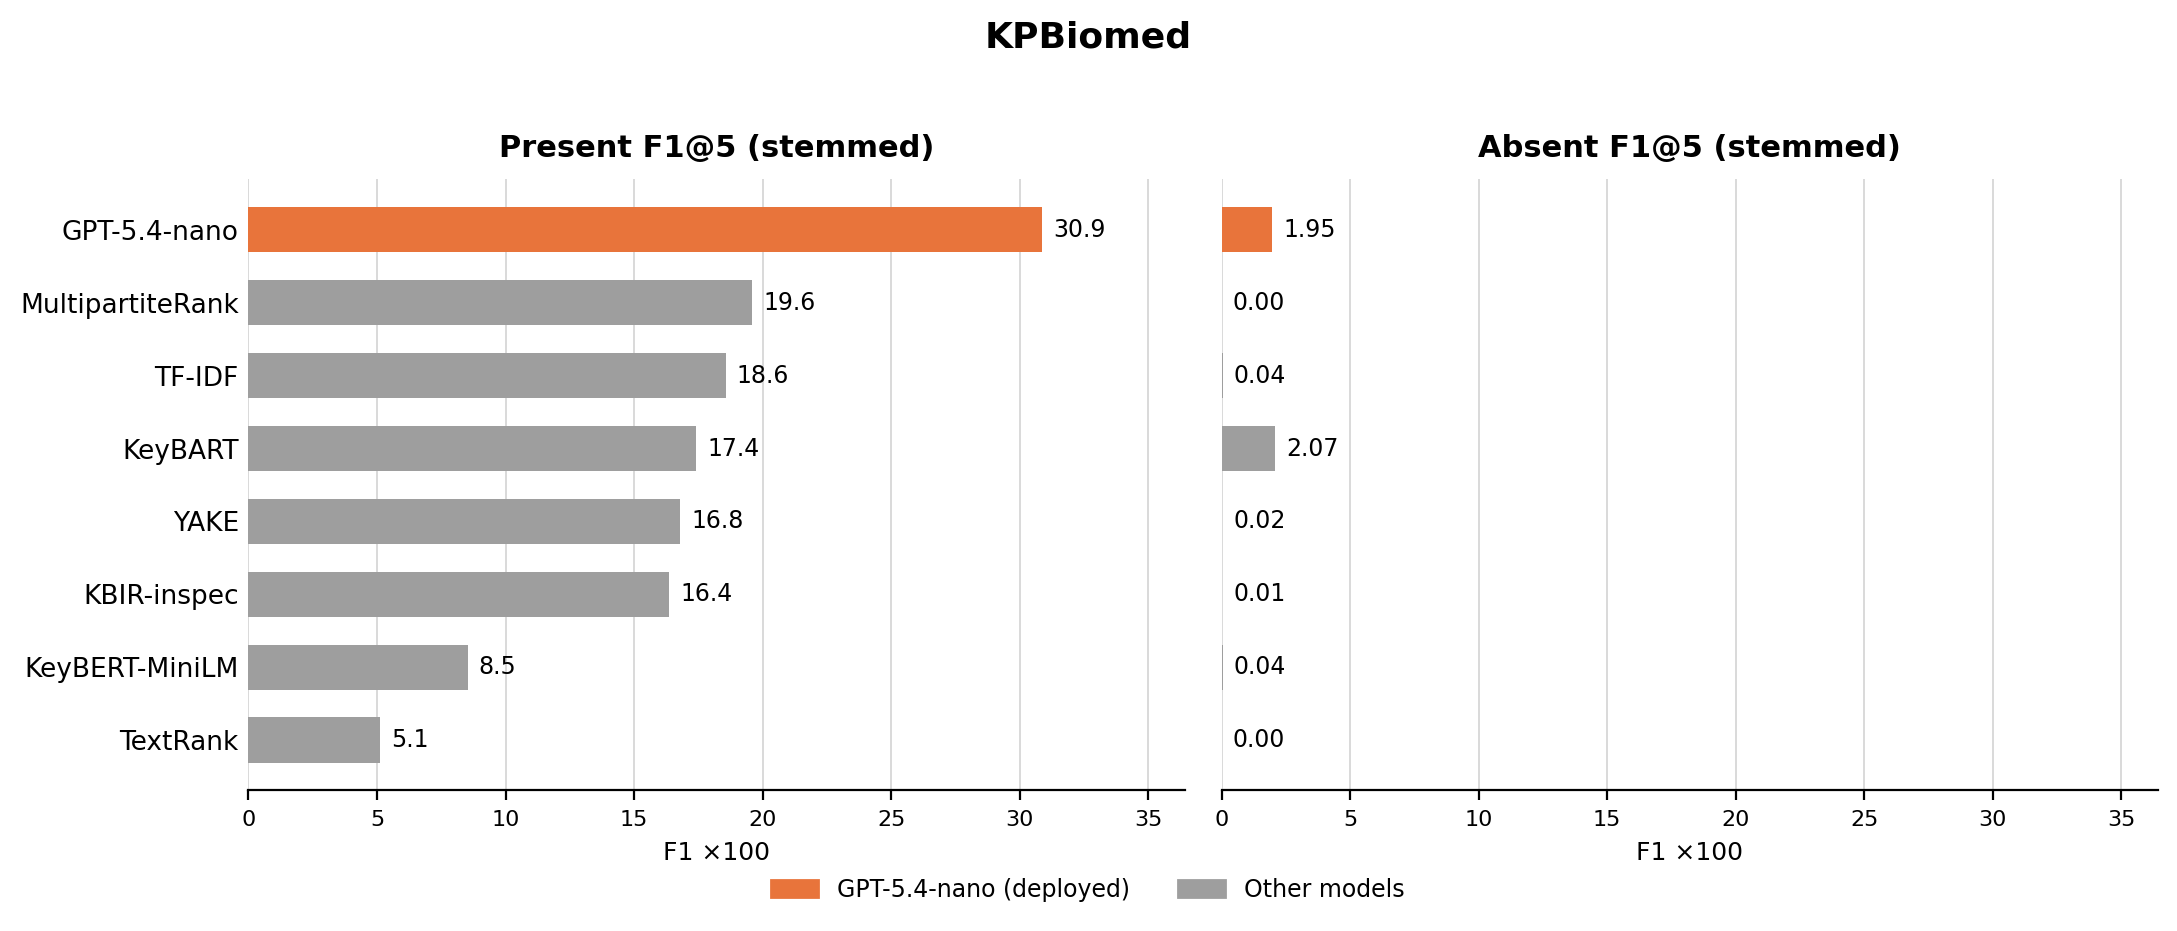
\includegraphics[width=\textwidth]{images/data_and_results/keyword_kpbiomed.png}
\caption{KPBiomed keyword extraction, present and absent F1@5 by model with stemming. The deployed model GPT-5.4-nano is shown in orange and the remaining baselines in grey.}
\label{fig:kw-kpbiomed}
\end{figure*}

\begin{table}[t]
\caption{OAGKX keyword extraction, present and absent F1@5 with stemming. Models are ordered by present F1, and GPT-5.4-nano is the deployed model.}
\label{tab:kw-oagkx}
\centering
\footnotesize
\begin{tabular}{@{}lrr@{}}
\toprule
Model & Present F1@5 & Absent F1@5 \\
\midrule
KeyBART & \textbf{28.42} & \textbf{5.09} \\
\textbf{GPT-5.4-nano} & 26.49 & 1.77 \\
KBIR-inspec & 20.16 & 0.05 \\
MultipartiteRank & 18.83 & 0.00 \\
TF-IDF & 15.55 & 0.03 \\
KeyBERT-MiniLM & 12.04 & 0.04 \\
TextRank & 11.15 & 0.02 \\
YAKE & 8.85 & 0.00 \\
\bottomrule
\end{tabular}
\end{table}

\begin{figure*}[t]
\centering
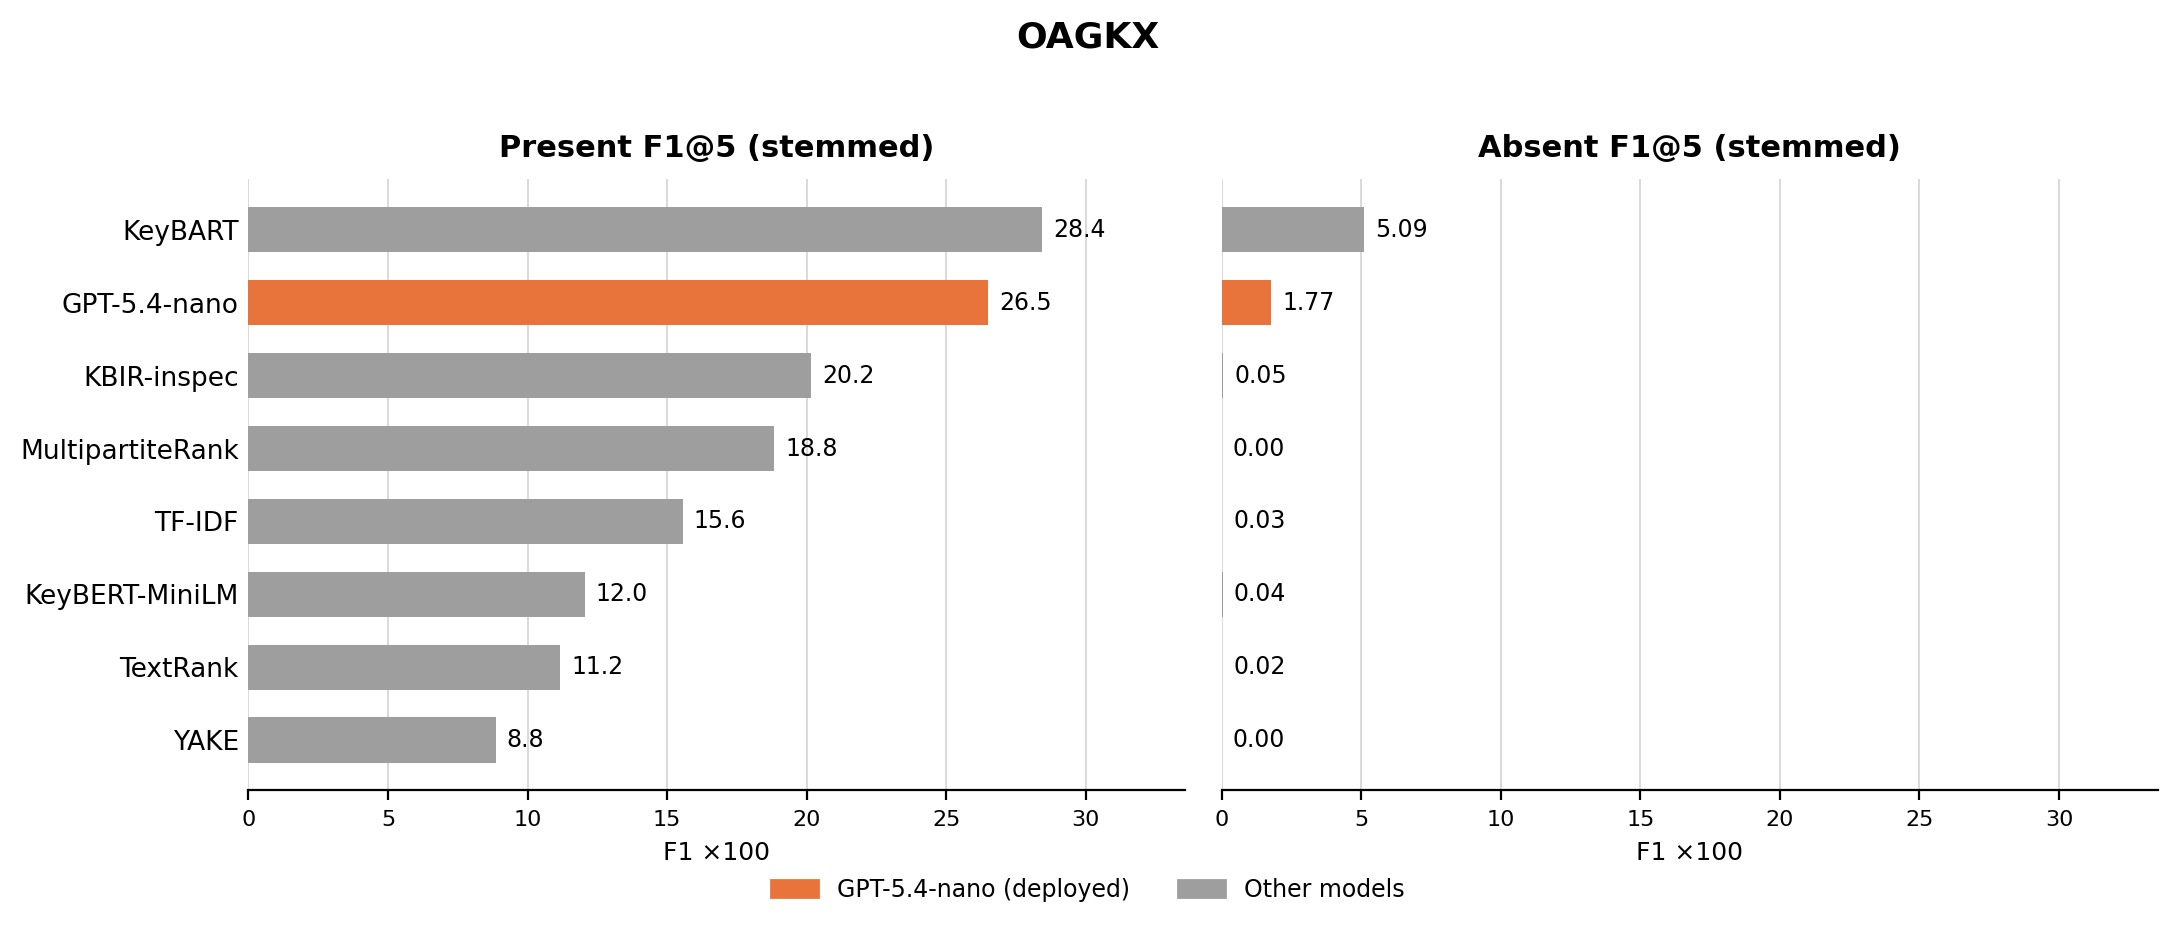
\includegraphics[width=\textwidth]{images/data_and_results/keyword_oagkx.png}
\caption{OAGKX keyword extraction, present and absent F1@5 by model with stemming. The deployed model GPT-5.4-nano is shown in orange and the remaining baselines in grey.}
\label{fig:kw-oagkx}
\end{figure*}

\begin{table}[t]
\caption{PubMedAKE keyword extraction, present and absent F1@5 with stemming. Models are ordered by present F1, and GPT-5.4-nano is the deployed model.}
\label{tab:kw-pubmedake}
\centering
\footnotesize
\begin{tabular}{@{}lrr@{}}
\toprule
Model & Present F1@5 & Absent F1@5 \\
\midrule
\textbf{GPT-5.4-nano} & \textbf{36.44} & \textbf{1.30} \\
TF-IDF & 24.06 & 0.03 \\
MultipartiteRank & 23.06 & 0.00 \\
KBIR-inspec & 19.36 & 0.01 \\
KeyBART & 18.41 & 1.29 \\
YAKE & 12.92 & 0.01 \\
KeyBERT-MiniLM & 6.78 & 0.01 \\
TextRank & 4.68 & 0.00 \\
\bottomrule
\end{tabular}
\end{table}

\begin{figure*}[t]
\centering
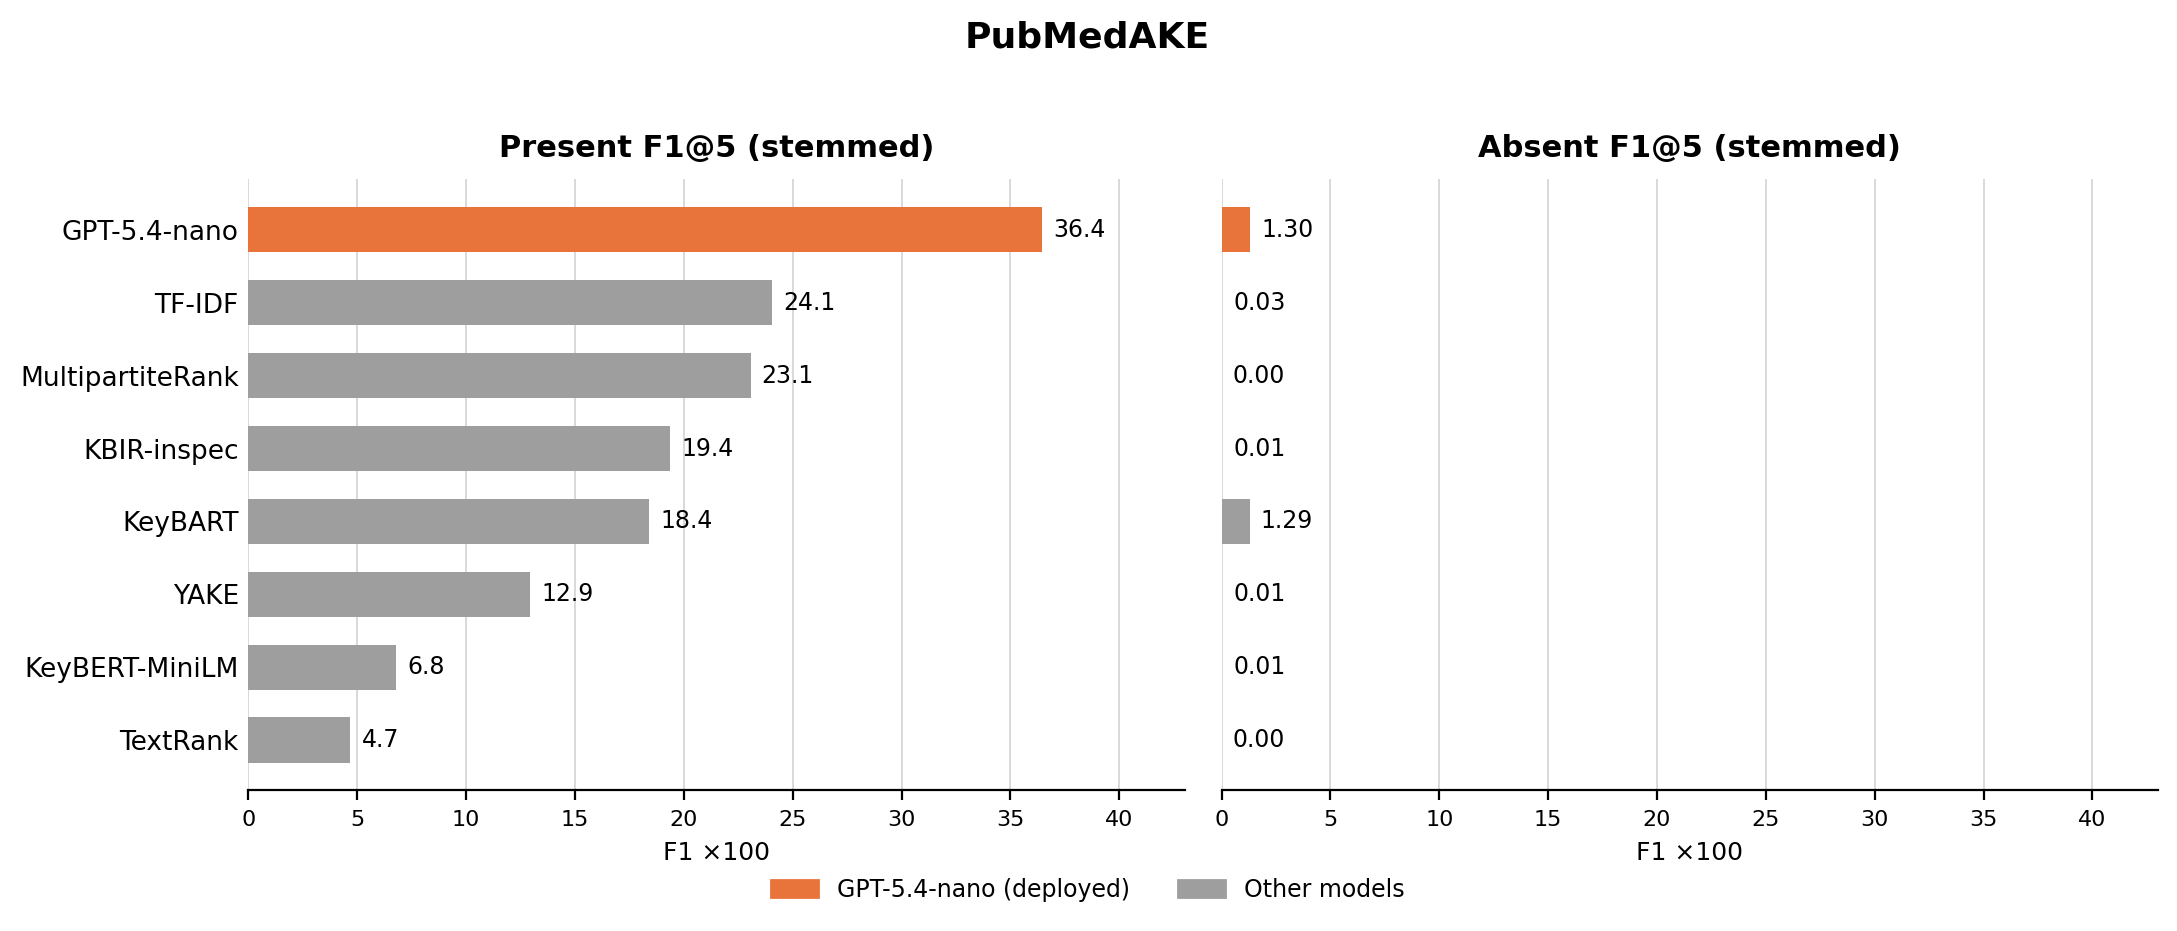
\includegraphics[width=\textwidth]{images/data_and_results/keyword_pubmedake.png}
\caption{PubMedAKE keyword extraction, present and absent F1@5 by model with stemming. The deployed model GPT-5.4-nano is shown in orange and the remaining baselines in grey.}
\label{fig:kw-pubmedake}
\end{figure*}

GPT-5.4-nano was benchmarked for keyword generation against a set of statistical and neural baselines on KPBiomed, OAGKX, and PubMedAKE. Tables~\ref{tab:kw-kpbiomed} to~\ref{tab:kw-pubmedake} report the results for each dataset in turn. Throughout, present (extractive) keyphrases, which occur verbatim in the source text, are distinguished from absent (abstractive) keyphrases, which do not and so must be generated. Matches are scored by F1 at five with light stemming, so that a keyphrase and its stem count as a match while a different word of the same meaning does not.

On the present keyphrase tasks, GPT-5.4-nano records the highest score on KPBiomed and PubMedAKE and the second highest on OAGKX, where KeyBART leads. Its margin is widest on PubMedAKE, at 36.44 against a next-best of 24.06.

On the absent keyphrase tasks, which a model can only score on by producing keyphrases that do not occur in the source text, GPT-5.4-nano scores in the low single digits, from 1.30 on PubMedAKE to 1.95 on KPBiomed. These non-zero scores indicate that the model generates a small portion of its keyphrases rather than extracting all of them. The other generative baseline, KeyBART, behaves similarly and records the highest absent score on KPBiomed and OAGKX. The statistical extractors such as TF-IDF, YAKE, TextRank, and MultipartiteRank remain near zero here, since they return only spans found in the source text and so do not generate at all.

\begin{table}[t]
\caption{Keyword extraction stability for GPT-5.4-nano over three runs on a 2000-document sample.}
\label{tab:kw-stability}
\centering
\footnotesize
\begin{tabular}{@{}p{0.66\columnwidth}r@{}}
\toprule
Quantity & Value \\
\midrule
Set-level Jaccard across runs & 0.73 \\
Present-F1 run-to-run std & $\pm$0.07 \\
Deterministic baselines (TF-IDF, YAKE, TextRank, MultipartiteRank, KeyBERT, KBIR) & 1.00 \\
\bottomrule
\end{tabular}
\end{table}

Table~\ref{tab:kw-stability} reports a reproducibility check for GPT-5.4-nano over three runs on a 2000-document sample. The set-level Jaccard similarity across runs is 0.73, meaning that for a given document around 73 percent of the combined set of keyphrases from any two runs is shared by both, equivalent to roughly one in six keyphrases changing between runs. The model is therefore largely repeatable but not deterministic, unlike the baselines, which are reproducible by construction. The effect on measured performance is negligible, with a run-to-run present-F1 standard deviation of 0.07. The same sample also reproduces the full-split figures to within roughly a tenth of a point, confirming that the smaller stability sample does not shift the headline results.

% ----------------------------------------------------------------------------
\subsection{IR Extraction}

\begin{table*}[t]
\caption{Natural-language-to-IR accuracy by model. Joint IR accuracy counts a query as correct when both its entities and its boolean expression are correct under exact matching, reported in the as-deployed or best configuration for each model.}
\label{tab:ir-accuracy}
\centering
\footnotesize
\begin{tabular}{@{}lllcc@{}}
\toprule
Model & Host & Configuration & IR accuracy & 95\% CI \\
\midrule
\textbf{gpt-5.4-nano} & Azure & default, 0 reasoning tok & \textbf{0.937}$^{\dagger}$ & [0.897, 0.983] \\
gpt-5-mini & Azure & default, 384 reasoning tok & 0.931 & [0.879, 0.974] \\
qwen3:8b & Local (Q4) & single-shot & 0.802 & [0.733, 0.871] \\
qwen3:4b & Local (Q4) & thinking$^{\ddagger}$ & 0.784 & [0.707, 0.862] \\
qwen2.5:3b & Local (Q4) & non-reasoning & 0.207 & [0.138, 0.284] \\
phi4-mini & Local (Q4) & non-reasoning & 0.052 & [0.017, 0.095] \\
llama3.2:3b & Local (Q4) & non-reasoning & 0.026 & [0.000, 0.060] \\
\bottomrule
\end{tabular}

\vspace{3pt}
\begin{minipage}{\linewidth}
\footnotesize\itshape
Confidence intervals are 95 percent bootstrap over 1000 iterations. Cross-model gaps that fall within these intervals are treated as ties, and bold marks the deployed model. The dagger denotes a three-run mean, whose single-run range is 0.914 to 0.940, with temperature zero returning a byte-identical output on 96.6 percent of queries (Table~\ref{tab:ir-stability}). The double dagger denotes qwen3:4b, whose single-shot configuration produced degenerate empty output, so its thinking configuration is its only usable score.
\end{minipage}
\end{table*}

\begin{figure}[t]
\centering
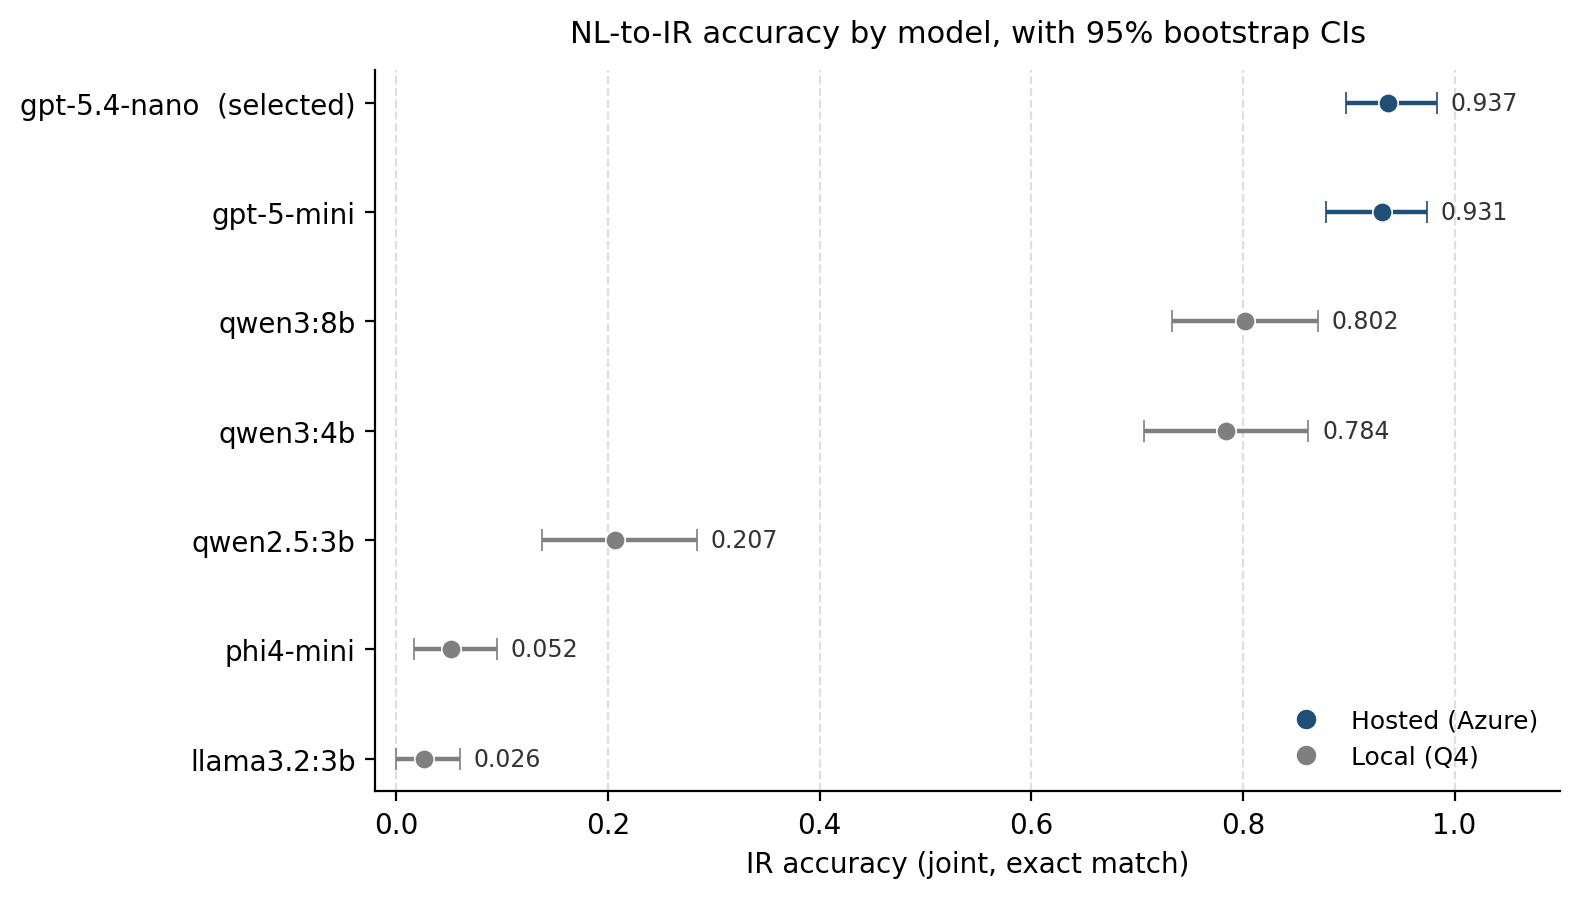
\includegraphics[width=\columnwidth]{images/data_and_results/ir_accuracy_ci.png}
\caption{Natural-language-to-IR joint accuracy by model on the hand-built gold set, with 95 percent bootstrap confidence intervals from 1000 resamples.}
\label{fig:ir-accuracy}
\end{figure}

GPT-5.4-nano was benchmarked for natural-language-to-IR extraction against a set of hosted and local models on a hand-built gold set of queries paired with their correct intermediate representations. The set was constructed to exercise every entity type the system supports across a range of boolean structures, from single topics through to bracketed combinations of AND, OR, and NOT, so that performance on it reflects the input and output behaviour the system actually requires. The headline measure, IR accuracy, is the joint figure reported in Table~\ref{tab:ir-accuracy}, counting a query as correct only when both its extracted entities and its boolean expression are correct under exact matching.

Figure~\ref{fig:ir-accuracy} plots each model's accuracy with its 95 percent bootstrap interval. The two hosted models lead the benchmark by a clear margin, with GPT-5.4-nano highest at an IR accuracy of 0.937 and GPT-5-mini close behind at 0.931. Both hosted intervals clear those of every local model without overlap, placing the hosted advantage beyond sampling noise, while the two overlap each other and are statistically indistinguishable. Among the local models, the two strongest (qwen3:8b and qwen3:4b) reach around 0.80, and the three smaller models fall away sharply to 0.207, 0.052, and 0.026, near the floor of the task.

\begin{table}[t]
\caption{Effect of reasoning on IR accuracy.}
\label{tab:ir-reasoning}
\centering
\footnotesize
\begin{tabular}{@{}lccc@{}}
\toprule
Model & Reasoning off & Reasoning on & $\Delta$ \\
\midrule
gpt-5.4-nano & 0.914 & 0.922 & +0.008 \\
gpt-5-mini & \textbf{0.750} & \textbf{0.940} & \textbf{+0.190} \\
\bottomrule
\end{tabular}

\vspace{3pt}
\begin{minipage}{\linewidth}
\footnotesize\itshape
Reasoning is controlled through the Azure \texttt{reasoning\_effort} setting with tokens accounted. Reasoning on used approximately 246 tokens per query for gpt-5.4-nano and 896 for gpt-5-mini, while reasoning off used none. Reasoning lifts the weaker model in each tier, while the stronger one is already at its ceiling.
\end{minipage}
\end{table}

Table~\ref{tab:ir-reasoning} isolates the effect of reasoning on the two GPT models. GPT-5.4-nano gains almost nothing from it, moving from 0.914 without reasoning to 0.922 with around 246 reasoning tokens, a difference of 0.008, and so reaches its accuracy in a single pass with no reasoning budget. GPT-5-mini behaves differently, scoring only 0.750 without reasoning and rising to 0.940 once reasoning is enabled, at a cost of around 896 reasoning tokens per query. The stronger model is already at its ceiling unaided, whereas the weaker one becomes competitive only by spending a substantial token budget.

\begin{table}[t]
\caption{Deployed model, metric decomposition in the default-effort configuration.}
\label{tab:ir-decomp}
\centering
\footnotesize
\begin{tabular}{@{}lcc@{}}
\toprule
Metric & Value & 95\% CI \\
\midrule
IR accuracy (joint) & 0.937 & [0.897, 0.983] \\
Entity F1 (micro) & 0.984 & [0.969, 0.995] \\
Entity F1 (macro) & 0.982 & [0.967, 0.994] \\
Expression equivalence & 0.931 & [0.888, 0.974] \\
Expression graded & 0.985 & [0.974, 0.995] \\
\bottomrule
\end{tabular}

\vspace{3pt}
\begin{minipage}{\linewidth}
\footnotesize\itshape
Joint accuracy is bounded by expression equivalence, since entity extraction almost never fails on its own.
\end{minipage}
\end{table}

\begin{table}[t]
\caption{Deployed model, accuracy by stratum, ordered hardest first.}
\label{tab:ir-stratum}
\centering
\footnotesize
\begin{tabular}{@{}lrrr@{}}
\toprule
Stratum & $n$ & IR accuracy & failures \\
\midrule
\texttt{filter\_distractor} & 10 & 0.700 & 3 \\
\texttt{multi\_negation} & 10 & 0.800 & 2 \\
\texttt{deep\_nested} & 12 & 0.833 & 2 \\
\texttt{hard\_typing} & 12 & 0.917 & 1 \\
\texttt{single\_concept} & 6 & 1.000 & 0 \\
\texttt{multi\_concept} & 12 & 1.000 & 0 \\
\texttt{exclusion} & 12 & 1.000 & 0 \\
\texttt{nested} & 12 & 1.000 & 0 \\
\texttt{mixed\_entity} & 16 & 1.000 & 0 \\
\texttt{review\_style} & 14 & 1.000 & 0 \\
\bottomrule
\end{tabular}

\vspace{3pt}
\begin{minipage}{\linewidth}
\footnotesize\itshape
The count $n$ is small per stratum, at sixteen or fewer, so the failure counts are a more reliable read than the rate, and the per-stratum 95 percent intervals are wide, for example \texttt{filter\_distractor} at 0.700 is seven of ten.
\end{minipage}
\end{table}

Tables~\ref{tab:ir-decomp} and~\ref{tab:ir-stratum} decompose the chosen model's performance, which is strong across both components and most query types. By component, entity extraction is near-perfect, with a micro F1 of 0.984 and a macro F1 of 0.982, while expression equivalence is lower at 0.931 (a graded variant that credits partially correct expressions reaches 0.985). The joint IR accuracy of 0.937 is therefore bounded by the expression score, since entity extraction almost never fails on its own. By query type, the model is perfect on six of the ten strata, covering single and multiple concepts, exclusions, nesting, mixed entities, and review-style queries. Its errors concentrate in the remaining four. The largest source is \texttt{filter\_distractor}, where three of ten queries fail because the model miscategorises a filter term such as a year or citation bound as a searchable entity. The rest fall on the structurally hardest queries, with two of ten failing on multiple negations, two of twelve on deep nesting, and one of twelve on hard typing. Per-stratum counts are small, at sixteen queries or fewer, so the failure counts are a more reliable read than the rates.

\begin{table}[t]
\caption{Stability of the deployed model over three runs.}
\label{tab:ir-stability}
\centering
\footnotesize
\begin{tabular}{@{}p{0.46\columnwidth}cc@{}}
\toprule
Metric & temp 0 & temp 0.7 \\
\midrule
IR identical across all 3 runs & 0.966 & 0.957 \\
Run-to-run IR-accuracy std & 0.004 & 0.004 \\
Majority-vote@3 vs single run & 0.931 vs 0.940 & 0.940 vs 0.940 \\
\bottomrule
\end{tabular}

\vspace{3pt}
\begin{minipage}{\linewidth}
\footnotesize\itshape
Temperature zero is highly but not perfectly deterministic, and majority voting adds nothing.
\end{minipage}
\end{table}

Table~\ref{tab:ir-stability} reports a stability check over three runs. Although GPT-5.4-nano is not deterministic, at temperature zero it returns an identical IR on 96.6 percent of queries, with a run-to-run accuracy standard deviation of 0.004. Aggregating three runs by majority vote changes nothing, at 0.931 against 0.940 for a single run, so the three-run mean of 0.937 reported in Table~\ref{tab:ir-accuracy} is used throughout.

% ----------------------------------------------------------------------------
\subsection{Dense Bi-encoder Retrieval}

\begin{table*}[t]
\caption{Dense bi-encoder retrieval on SciRepEval ad-hoc search, nDCG $\times$100 with 95 percent bootstrap confidence intervals.}
\label{tab:bienc-results}
\centering
\scriptsize
\setlength{\tabcolsep}{4pt}
\begin{tabular}{@{}p{3.0cm}llll@{}}
\toprule
Model & NFCorpus & TREC-CoVID & Search & Average \\
\midrule
Qwen3-Embedding-4B (int8) & \textbf{80.02 [77.75, 82.17]} & \textbf{94.28 [92.96, 95.43]} & 75.54 [74.93, 76.17] & \textbf{83.28 [82.35, 84.19]} \\
EmbeddingGemma-300M & 79.13 [76.84, 81.29] & 92.45 [90.68, 94.03] & 75.32 [74.66, 75.93] & 82.30 [81.32, 83.31] \\
Qwen3-Embedding-0.6B & 77.94 [75.75, 80.22] & 93.90 [92.52, 95.10] & 75.03 [74.41, 75.65] & 82.29 [81.32, 83.25] \\
text-embedding-3-small (existing) & 78.78 [76.61, 81.05] & 92.38 [90.58, 93.96] & 75.14 [74.52, 75.74] & 82.10 [81.08, 83.05] \\
mxbai-embed-large-v1 & 79.37 [77.19, 81.72] & 91.77 [90.02, 93.25] & 74.92 [74.29, 75.56] & 82.02 [81.06, 82.96] \\
SPECTER2-adhoc-query & 70.46 [68.01, 72.97] & 90.08 [87.84, 92.13] & \textbf{78.22 [77.60, 78.86]} & 79.59 [78.46, 80.71] \\
BGE-M3 & 74.05 [71.72, 76.35] & 89.21 [87.08, 91.16] & 74.82 [74.20, 75.46] & 79.36 [78.29, 80.42] \\
SPECTER2-base (existing) & 72.03 [69.60, 74.54] & 89.46 [86.99, 91.58] & 73.76 [73.12, 74.41] & 78.42 [77.27, 79.58] \\
\bottomrule
\end{tabular}

\vspace{3pt}
\begin{minipage}{\linewidth}
\footnotesize\itshape
The metric is SciRepEval ad-hoc-search full-ranking nDCG over a per-query candidate pool, not BEIR full-corpus nDCG@10. Confidence intervals are 95 percent bootstrap [lo, hi] over 1000 iterations with seed 42, and bold marks the best point estimate per column. On Average the top five models' intervals overlap, a statistical tie, and SPECTER2-adhoc-query's Search lead is the one between-model gap whose interval clears the general models.
\end{minipage}
\end{table*}

\begin{figure}[t]
\centering
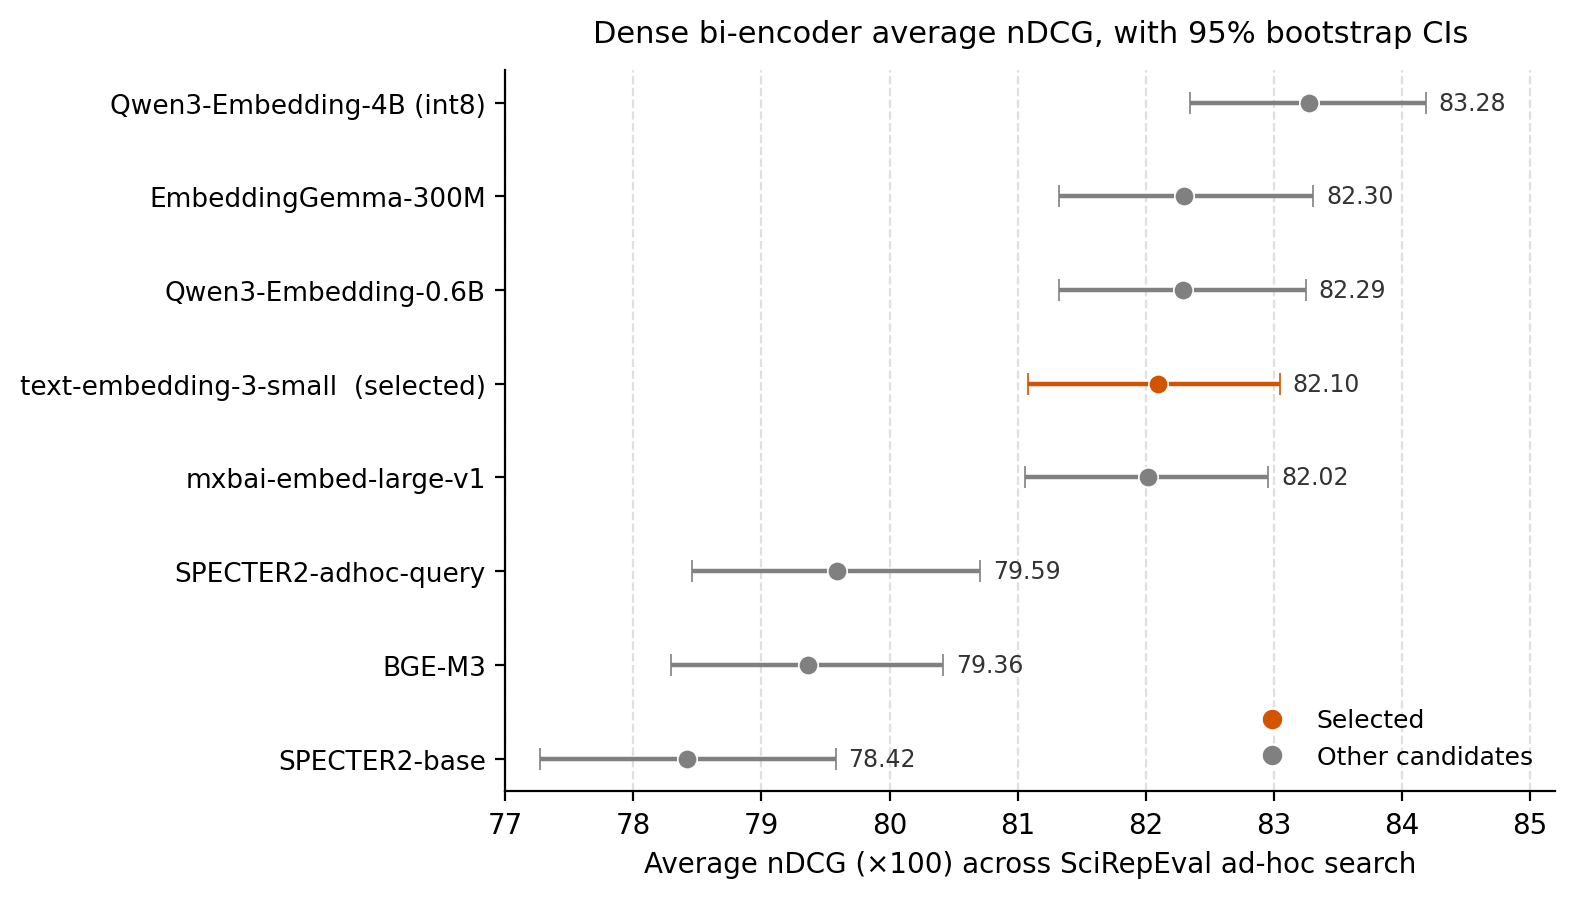
\includegraphics[width=\columnwidth]{images/data_and_results/biencoder_average.png}
\caption{Dense bi-encoder average nDCG across the three SciRepEval ad-hoc search tasks, with 95 percent bootstrap confidence intervals from 1000 resamples. The selected model is shown in orange.}
\label{fig:bienc-avg}
\end{figure}

\begin{figure}[t]
\centering
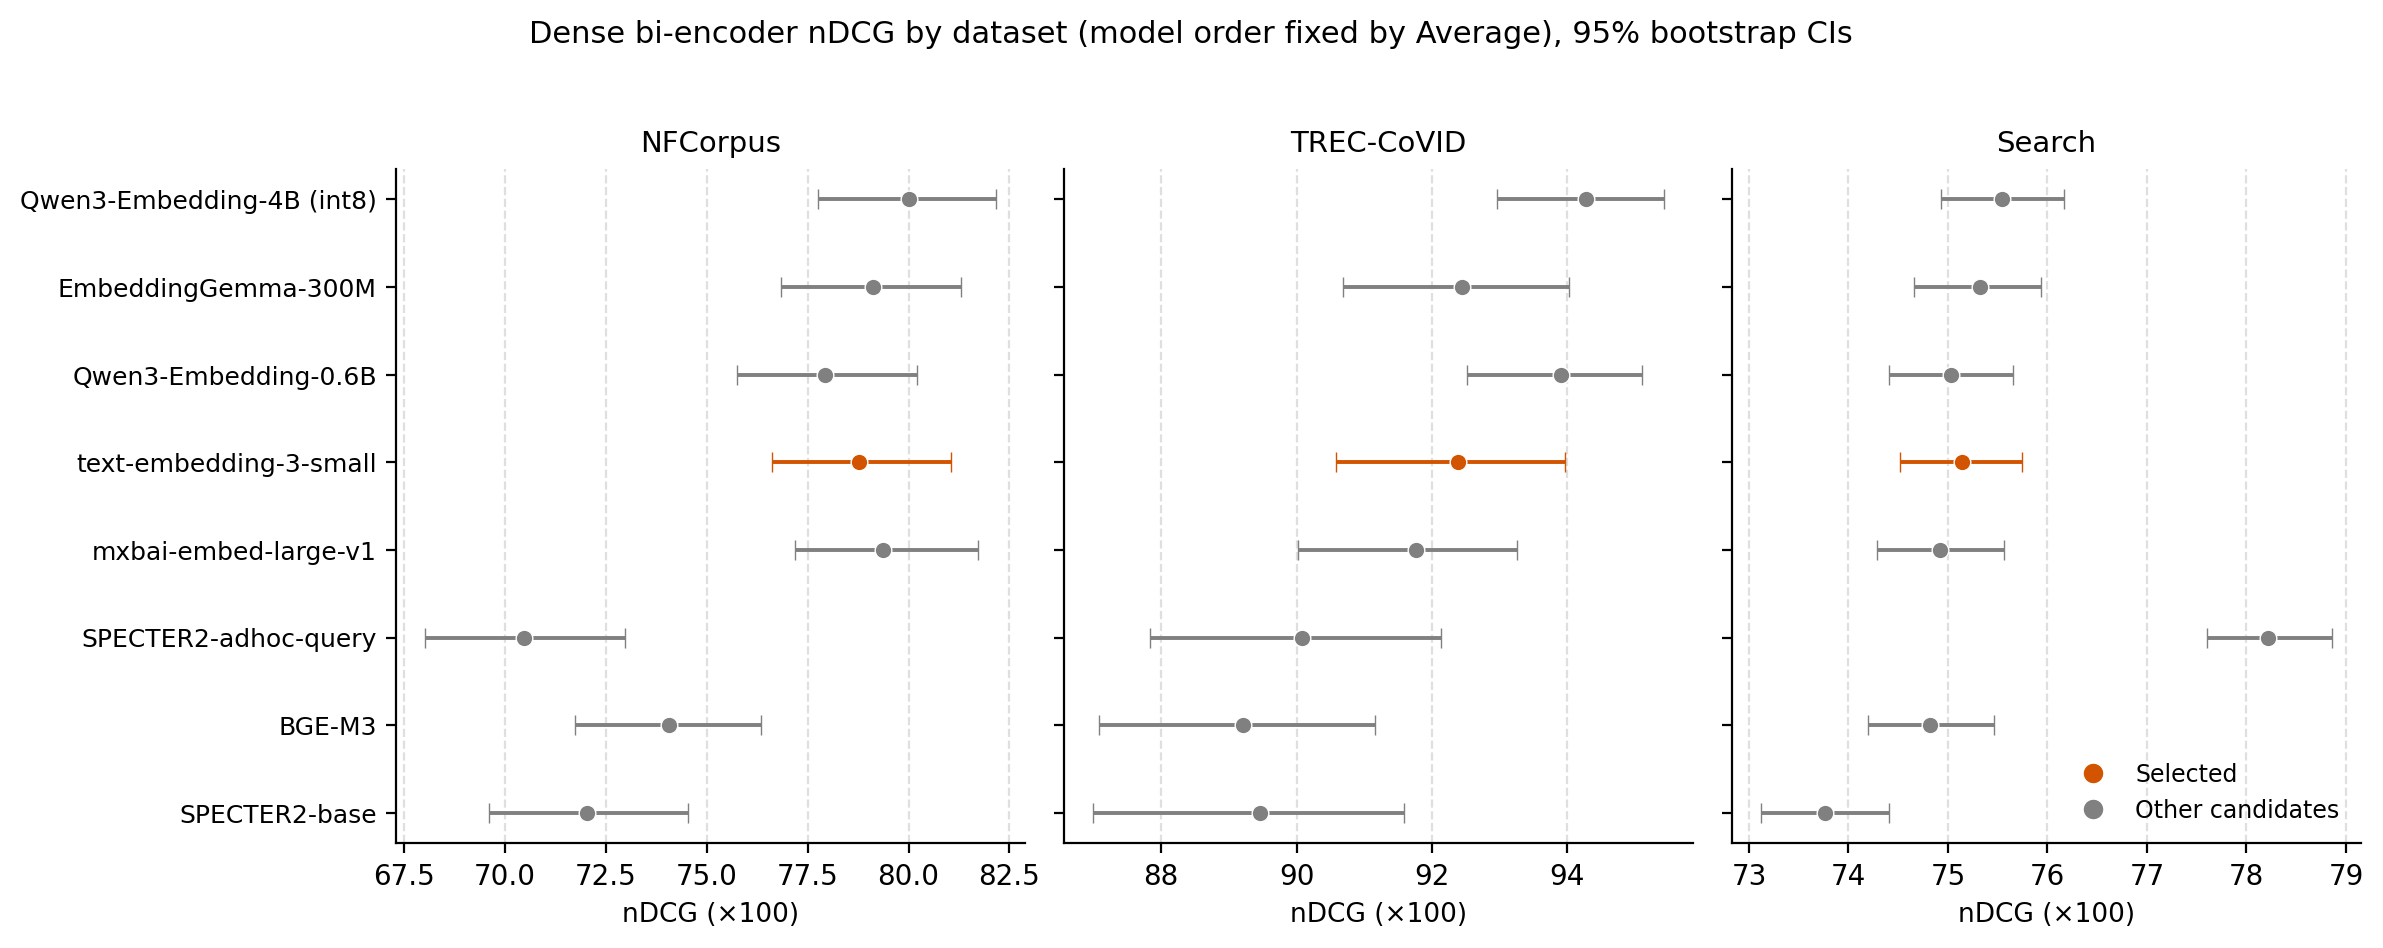
\includegraphics[width=\columnwidth]{images/data_and_results/biencoder_by_dataset.png}
\caption{Dense bi-encoder nDCG on each SciRepEval ad-hoc search task, with models held in their Average order for comparison and 95 percent bootstrap confidence intervals. The selected model is shown in orange.}
\label{fig:bienc-pertask}
\end{figure}

text-embedding-3-small was selected as the dense bi-encoder. The candidate models were evaluated on the three ad-hoc search tasks of SciRepEval, namely NFCorpus, TREC-CoVID, and Search, scored by nDCG. The figure reported is SciRepEval full-ranking nDCG over a per-query candidate pool rather than BEIR full-corpus nDCG@10, which keeps the stage comparable to the scientific retrieval benchmark established in Section~II-D. All scores are nDCG $\times$100 with 95 percent bootstrap intervals from 1000 resamples.

Table~\ref{tab:bienc-results} reports the per-task and average scores in full, and Figure~\ref{fig:bienc-avg} plots each model's average nDCG with its interval. The selected model records an average of 82.10. Qwen3-Embedding-4B holds the highest point estimate at 83.28, but the intervals of the top five models all overlap, forming a statistical tie that contains text-embedding-3-small along with EmbeddingGemma-300M, Qwen3-Embedding-0.6B, and mxbai-embed-large-v1. A clear margin separates this group from the lower three, SPECTER2-adhoc-query at 79.59, BGE-M3 at 79.36, and SPECTER2-base at 78.42, whose intervals fall below the leading cluster.

The average conceals a difference in where each model does its work, shown per task in Figure~\ref{fig:bienc-pertask}. On NFCorpus and TREC-CoVID the general-purpose embedders lead, with Qwen3-Embedding-4B highest on both. On Search the order changes. SPECTER2-adhoc-query scores 78.22 against a field clustered near 75, and this is the single between-model gap on any one task whose interval clears the general models. The same model is weakest on NFCorpus at 70.46, so its Search lead does not survive into the average. The selected model sits within the leading group on each of the three tasks.

\begin{table*}[t]
\caption{Deployment characteristics of the candidate bi-encoders.}
\label{tab:bienc-deploy}
\centering
\footnotesize
\begin{tabular}{@{}lllll@{}}
\toprule
Model & Params (approx.) & Embedding dim & Precision & Self-hostable \\
\midrule
Qwen3-Embedding-4B & $\sim$4 B & 2560 & int8 & yes \\
EmbeddingGemma-300M & $\sim$300 M & 768 & fp16 & yes \\
Qwen3-Embedding-0.6B & $\sim$0.6 B & 1024 & fp16 & yes \\
text-embedding-3-small & undisclosed & 1536 & n/a & no (paid API) \\
mxbai-embed-large-v1 & $\sim$335 M & 1024 & fp16 & yes \\
SPECTER2-adhoc-query & $\sim$110 M & 768 & fp16 & yes \\
BGE-M3 & $\sim$568 M & 1024 & fp16 & yes \\
SPECTER2-base & $\sim$110 M & 768 & fp16 & yes \\
\bottomrule
\end{tabular}

\vspace{3pt}
\begin{minipage}{\linewidth}
\footnotesize\itshape
In-memory footprint per stored vector scales with embedding dimension at int8, at roughly one byte per dimension, giving around 65 GB at 768 dimensions, 87 GB at 1024, 131 GB at 1536, and 218 GB at 2560 over the 85 million works. Encoding cost scales with parameter count.
\end{minipage}
\end{table*}

Table~\ref{tab:bienc-deploy} records the deployment characteristics that the nDCG scores do not, namely approximate parameter count, embedding dimension, precision, and whether the model is self-hostable. In-memory footprint per stored vector scales with embedding dimension at int8, from around 65 GB at 768 dimensions to around 218 GB at 2560 dimensions over the 85 million works, while encoding cost scales with parameter count. The selected model has an embedding dimension of 1536, placing its footprint at around 131 GB, and is served through a paid API rather than self-hosted.

% ----------------------------------------------------------------------------
\subsection{Cross-encoder Re-ranking}

\begin{table*}[t]
\caption{Cross-encoder re-ranking on SciRepEval ad-hoc search, nDCG $\times$100 with 95 percent bootstrap confidence intervals, sorted by Average.}
\label{tab:xenc-results}
\centering
\scriptsize
\setlength{\tabcolsep}{4pt}
\begin{tabular}{@{}p{3.2cm}llll@{}}
\toprule
Model (scorer) & NFCorpus & TREC-CoVID & Search & Average \\
\midrule
Cohere Rerank 4.0 Pro (API) & \textbf{80.42 [78.17, 82.60]} & \textbf{94.60 [93.30, 95.71]} & 75.39 [74.76, 76.00] & \textbf{83.47 [82.54, 84.33]} \\
Qwen3-Reranker-4B (int8) & 80.10 [77.94, 82.14] & 94.37 [92.90, 95.60] & 74.93 [74.32, 75.56] & 83.13 [82.18, 83.99] \\
Cohere Rerank 4.0 Fast (API) & 78.77 [76.55, 80.98] & 94.15 [92.83, 95.31] & \textbf{75.42 [74.75, 76.04]} & 82.78 [81.83, 83.68] \\
Qwen3-Reranker-0.6B (fp16) & 78.06 [75.65, 80.24] & 93.98 [92.59, 95.20] & 75.25 [74.59, 75.85] & 82.43 [81.50, 83.34] \\
mxbai-rerank-large-v1 (435M) & 78.32 [76.08, 80.76] & 91.50 [89.43, 93.33] & 74.78 [74.15, 75.46] & 81.53 [80.48, 82.59] \\
jina-reranker-v2-base (278M) & 76.73 [74.49, 79.01] & 91.84 [90.05, 93.52] & 75.37 [74.73, 75.99] & 81.31 [80.28, 82.30] \\
MedCPT-Cross-Encoder (109M, biomed) & 75.70 [73.21, 78.03] & 88.91 [86.61, 90.97] & 73.97 [73.34, 74.63] & 79.53 [78.40, 80.66] \\
ms-marco-MiniLM-L-6-v2 (22M) & 73.10 [70.78, 75.48] & 88.78 [86.41, 90.90] & 75.21 [74.58, 75.84] & 79.03 [77.90, 80.13] \\
bge-reranker-v2-m3 (568M) & 70.71 [68.31, 73.07] & 90.30 [88.29, 92.18] & 74.40 [73.78, 75.05] & 78.47 [77.37, 79.53] \\
ms-marco-MiniLM-L-12-v2 (33M) & 69.88 [67.41, 72.38] & 87.17 [84.73, 89.52] & 75.09 [74.44, 75.71] & 77.38 [76.17, 78.54] \\
bge-reranker-large (560M) & 66.49 [64.11, 68.85] & 87.27 [84.61, 89.62] & 74.22 [73.59, 74.85] & 76.00 [74.80, 77.16] \\
bge-reranker-base (278M) & 58.75 [56.38, 60.94] & 84.98 [82.12, 87.60] & 72.60 [71.97, 73.24] & 72.11 [70.84, 73.35] \\
gte-reranker-modernbert-base (150M) & 48.88 [46.82, 50.93] & 79.03 [76.40, 81.60] & 69.94 [69.26, 70.60] & 65.95 [64.91, 67.07] \\
\bottomrule
\end{tabular}

\vspace{3pt}
\begin{minipage}{\linewidth}
\footnotesize\itshape
The metric is SciRepEval ad-hoc-search full-ranking nDCG over a reranking pool, not BEIR full-corpus nDCG@10. Confidence intervals are 95 percent bootstrap [2.5 percent, 97.5 percent] over 1000 iterations with seed 42, with the Average resampled independently within each dataset. The intervals are tight on Search, which has 2585 queries, and wide on TREC-CoVID, which has 50, and bold marks the best point estimate per column. The top four models, namely Cohere Pro, Qwen3-Reranker-4B, Cohere Fast, and Qwen3-Reranker-0.6B, have heavily overlapping Average intervals and form a statistical tie, within which the best self-hostable model, Qwen3-Reranker-4B at int8, is tied with Cohere Pro. On Search the small candidate pool saturates every reranker at around 75. For reference, the bi-encoder embeddings without intervals give the best embedder Qwen3-Embedding-4B at 83.28 Average, SPECTER2-adhoc-query at 78.22 on Search, which is above every reranker here, and text-embedding-3-small at 82.10 Average.
\end{minipage}
\end{table*}

\begin{figure}[t]
\centering
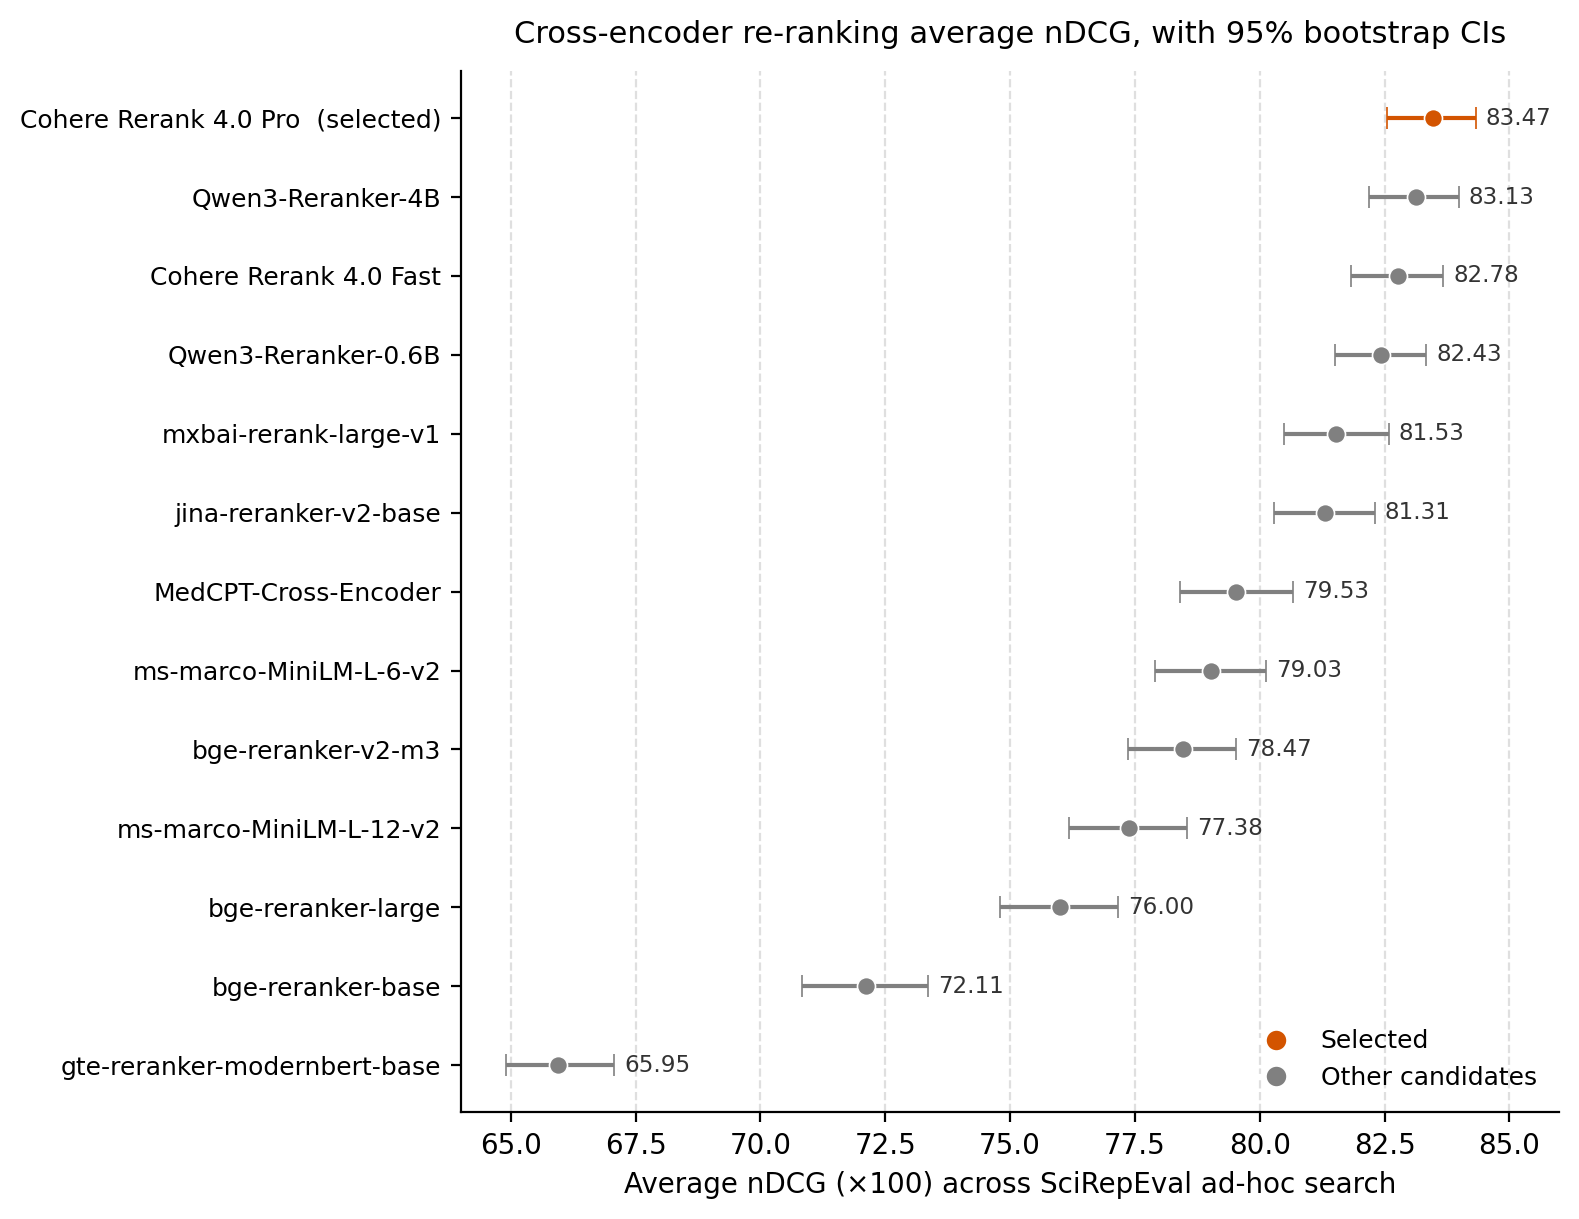
\includegraphics[width=\columnwidth]{images/data_and_results/crossencoder_average.png}
\caption{Cross-encoder re-ranking average nDCG across the three SciRepEval ad-hoc search tasks, with 95 percent bootstrap confidence intervals from 1000 resamples. The selected model is shown in orange.}
\label{fig:xenc-avg}
\end{figure}

\begin{figure}[t]
\centering
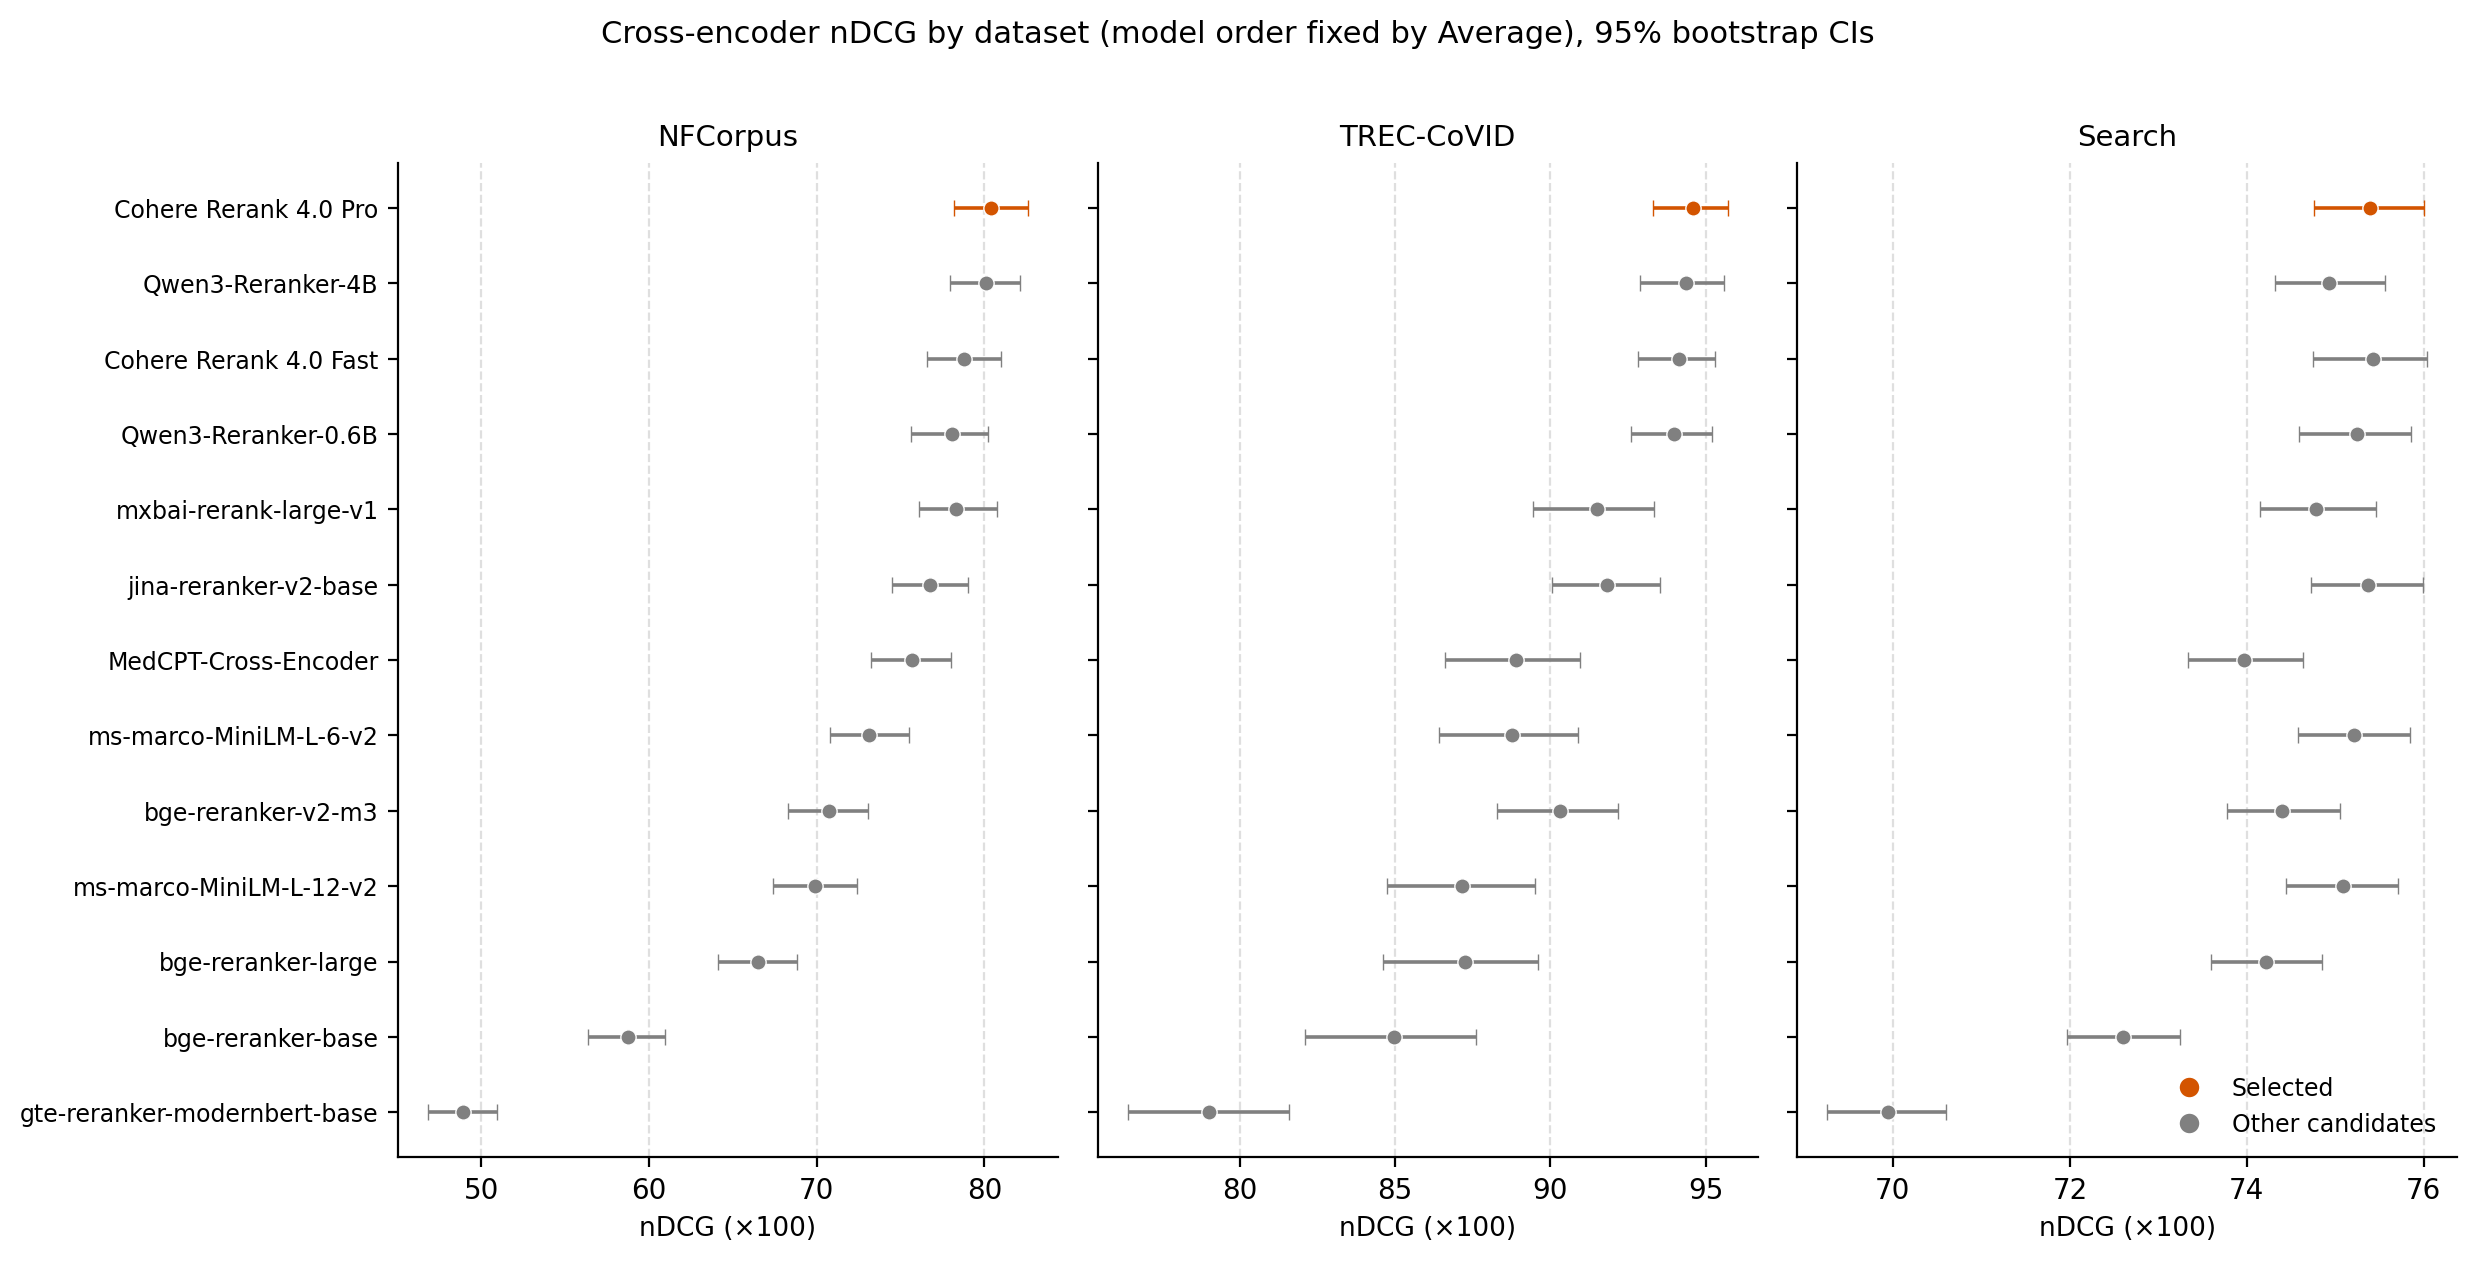
\includegraphics[width=\columnwidth]{images/data_and_results/crossencoder_by_dataset.png}
\caption{Cross-encoder nDCG on each SciRepEval ad-hoc search task, with models held in their Average order for comparison and 95 percent bootstrap confidence intervals. The selected model is shown in orange.}
\label{fig:xenc-pertask}
\end{figure}

Cohere Rerank 4.0 Pro was selected as the cross-encoder. The candidate rerankers were evaluated on the same three SciRepEval ad-hoc search tasks as the bi-encoder and under the same nDCG metric, scoring each model by the ranking it produces when it re-ranks the retrieved candidate pool. All scores are nDCG $\times$100 with 95 percent bootstrap intervals from 1000 resamples. The intervals are tight on Search, which has 2585 queries, and wide on TREC-CoVID, which has 50.

Table~\ref{tab:xenc-results} reports the full per-task and average scores, and Figure~\ref{fig:xenc-avg} plots each model's average with its interval. The selected model holds the highest average at 83.47. Its interval overlaps those of the next three models, Qwen3-Reranker-4B at 83.13, Cohere Rerank 4.0 Fast at 82.78, and Qwen3-Reranker-0.6B at 82.43, so these four form a statistical tie at the top. Within that group the strongest self-hostable model, Qwen3-Reranker-4B, is tied with the selected model. Below the leading four the field descends steadily through a long tail to gte-reranker-modernbert-base at 65.95, a spread of more than seventeen points from top to bottom.

The per-task view in Figure~\ref{fig:xenc-pertask} shows that almost all of this separation comes from NFCorpus, where the models spread across more than thirty points, from 80.42 at the top down to 48.88. Search behaves in the opposite way. Every reranker scores close to 75, since the small candidate pool the stage re-ranks leaves little room to reorder, so the task barely separates the models. TREC-CoVID falls between the two, with a high but noisy spread that reflects its fifty queries.

\begin{table*}[t]
\caption{Deployment characteristics of the candidate cross-encoders.}
\label{tab:xenc-deploy}
\centering
\footnotesize
\begin{tabular}{@{}p{4.5cm}llp{4.0cm}@{}}
\toprule
Model & Params (approx.) & Precision & Self-hostable \\
\midrule
Cohere Rerank 4.0 Pro & undisclosed & n/a & no (paid API) \\
Qwen3-Reranker-4B & $\sim$4 B & int8 & yes (Apache-2.0) \\
Cohere Rerank 4.0 Fast & undisclosed & n/a & no (paid API) \\
Qwen3-Reranker-0.6B & $\sim$0.6 B & fp16 & yes (Apache-2.0) \\
mxbai-rerank-large-v1 & $\sim$435 M & fp16 & yes \\
jina-reranker-v2-base & $\sim$278 M & fp16 & weights CC-BY-NC (non-commercial) \\
MedCPT-Cross-Encoder & $\sim$109 M & fp16 & yes \\
ms-marco-MiniLM-L-6-v2 & $\sim$22 M & fp16 & yes \\
bge-reranker-v2-m3 & $\sim$568 M & fp16 & yes \\
ms-marco-MiniLM-L-12-v2 & $\sim$33 M & fp16 & yes \\
bge-reranker-large & $\sim$560 M & fp16 & yes \\
bge-reranker-base & $\sim$278 M & fp16 & yes \\
gte-reranker-modernbert-base & $\sim$150 M & fp16 & yes \\
\bottomrule
\end{tabular}

\vspace{3pt}
\begin{minipage}{\linewidth}
\footnotesize\itshape
Unlike the bi-encoder, a reranker stores no vectors, so its cost is latency, which scales with parameter count, rather than memory, which is why the stage runs over only around 100 candidates. The Qwen3 rerankers are released under Apache-2.0, while the jina-reranker-v2 weights are CC-BY-NC-4.0 and so are non-commercial and not deployable in a commercial product. The remaining licences should be confirmed against the deployment terms before selection.
\end{minipage}
\end{table*}

Table~\ref{tab:xenc-deploy} records the deployment characteristics, namely approximate parameter count, precision, and whether the model is self-hostable along with its licence. Unlike the bi-encoder, a reranker stores no vectors, so its cost is latency rather than memory and scales with parameter count, which is the reason the stage runs over only around 100 candidates. The self-hostable options carry mixed licences, with the Qwen3 rerankers released under Apache-2.0 and the jina reranker under a non-commercial CC-BY-NC licence, while the selected model is served through a paid API.

% ----------------------------------------------------------------------------
\subsection{Embedding Quantisation}
% Placeholder. Results not yet available.
\textit{[Placeholder. Results comparing int8 against full-precision nDCG, and the resulting accuracy cost, to be added.]}

% ----------------------------------------------------------------------------
\subsection{System-Level Evaluation}
% Placeholder. Results not yet available.
\textit{[Placeholder. End-to-end results over a realistic query set with light relevance judgments to be added.]}   (or \include{...})
%
%  Requires in the preamble of main.tex:
%      \usepackage{booktabs}
%      \usepackage{graphicx}
%      \usepackage{array}      % only if you later add >{...} column types
%
%  Figures use placeholder paths under figures/ -- replace with your exports.
%  Tables and figures are referenced with \ref so numbering stays dynamic and
%  any table can be moved to an appendix without breaking the prose.
% ============================================================================

\section{Data and Results}

This section reports the result of each component benchmark from the validation design in Section~II-D, taking the components in turn.

% ----------------------------------------------------------------------------
\subsection{Keyword Generation}

\begin{table}[t]
\caption{KPBiomed keyword extraction, present and absent F1@5 with stemming. Models are ordered by present F1, and GPT-5.4-nano is the deployed model.}
\label{tab:kw-kpbiomed}
\centering
\footnotesize
\begin{tabular}{@{}lrr@{}}
\toprule
Model & Present F1@5 & Absent F1@5 \\
\midrule
\textbf{GPT-5.4-nano} & \textbf{30.86} & 1.95 \\
MultipartiteRank & 19.58 & 0.00 \\
TF-IDF & 18.56 & 0.04 \\
KeyBART & 17.40 & \textbf{2.07} \\
YAKE & 16.79 & 0.02 \\
KBIR-inspec & 16.36 & 0.01 \\
KeyBERT-MiniLM & 8.52 & 0.04 \\
TextRank & 5.11 & 0.00 \\
\bottomrule
\end{tabular}
\end{table}

\begin{figure*}[t]
\centering
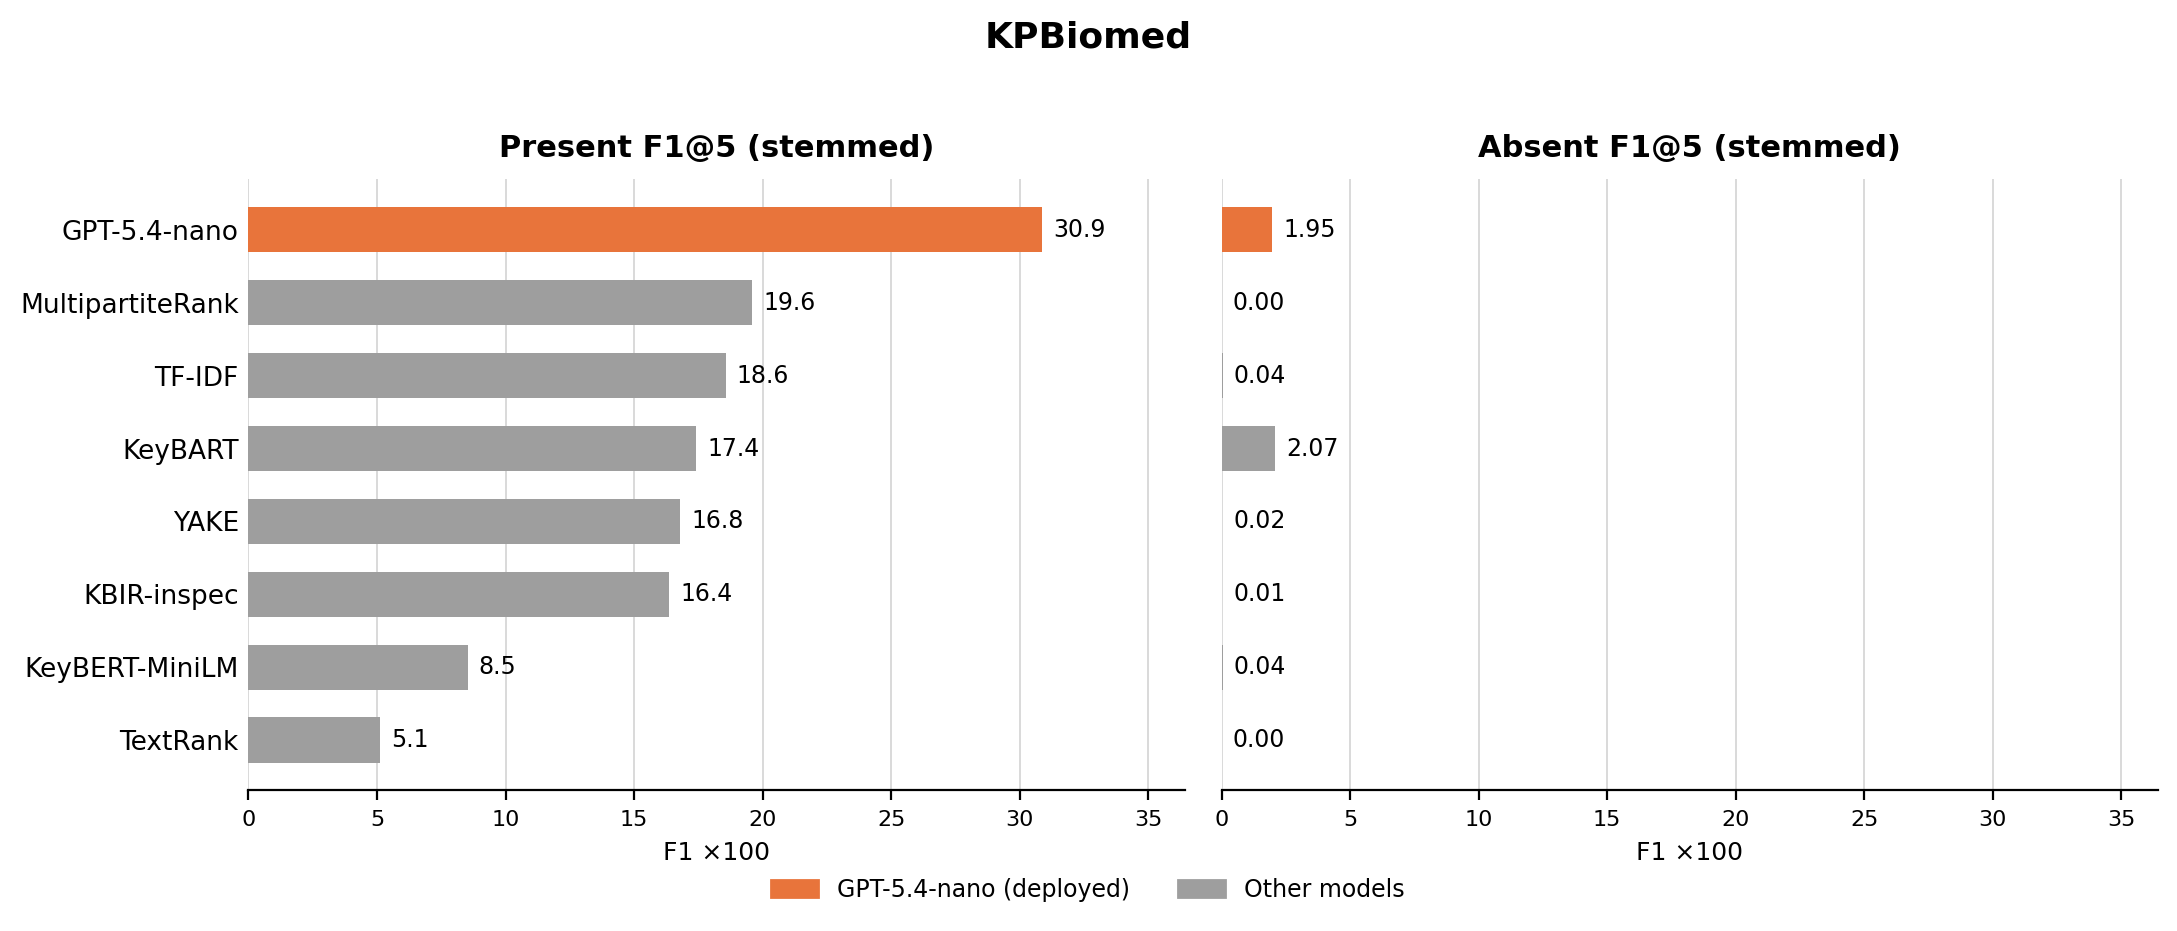
\includegraphics[width=\textwidth]{images/data_and_results/keyword_kpbiomed.png}
\caption{KPBiomed keyword extraction, present and absent F1@5 by model with stemming. The deployed model GPT-5.4-nano is shown in orange and the remaining baselines in grey.}
\label{fig:kw-kpbiomed}
\end{figure*}

\begin{table}[t]
\caption{OAGKX keyword extraction, present and absent F1@5 with stemming. Models are ordered by present F1, and GPT-5.4-nano is the deployed model.}
\label{tab:kw-oagkx}
\centering
\footnotesize
\begin{tabular}{@{}lrr@{}}
\toprule
Model & Present F1@5 & Absent F1@5 \\
\midrule
KeyBART & \textbf{28.42} & \textbf{5.09} \\
\textbf{GPT-5.4-nano} & 26.49 & 1.77 \\
KBIR-inspec & 20.16 & 0.05 \\
MultipartiteRank & 18.83 & 0.00 \\
TF-IDF & 15.55 & 0.03 \\
KeyBERT-MiniLM & 12.04 & 0.04 \\
TextRank & 11.15 & 0.02 \\
YAKE & 8.85 & 0.00 \\
\bottomrule
\end{tabular}
\end{table}

\begin{figure*}[t]
\centering
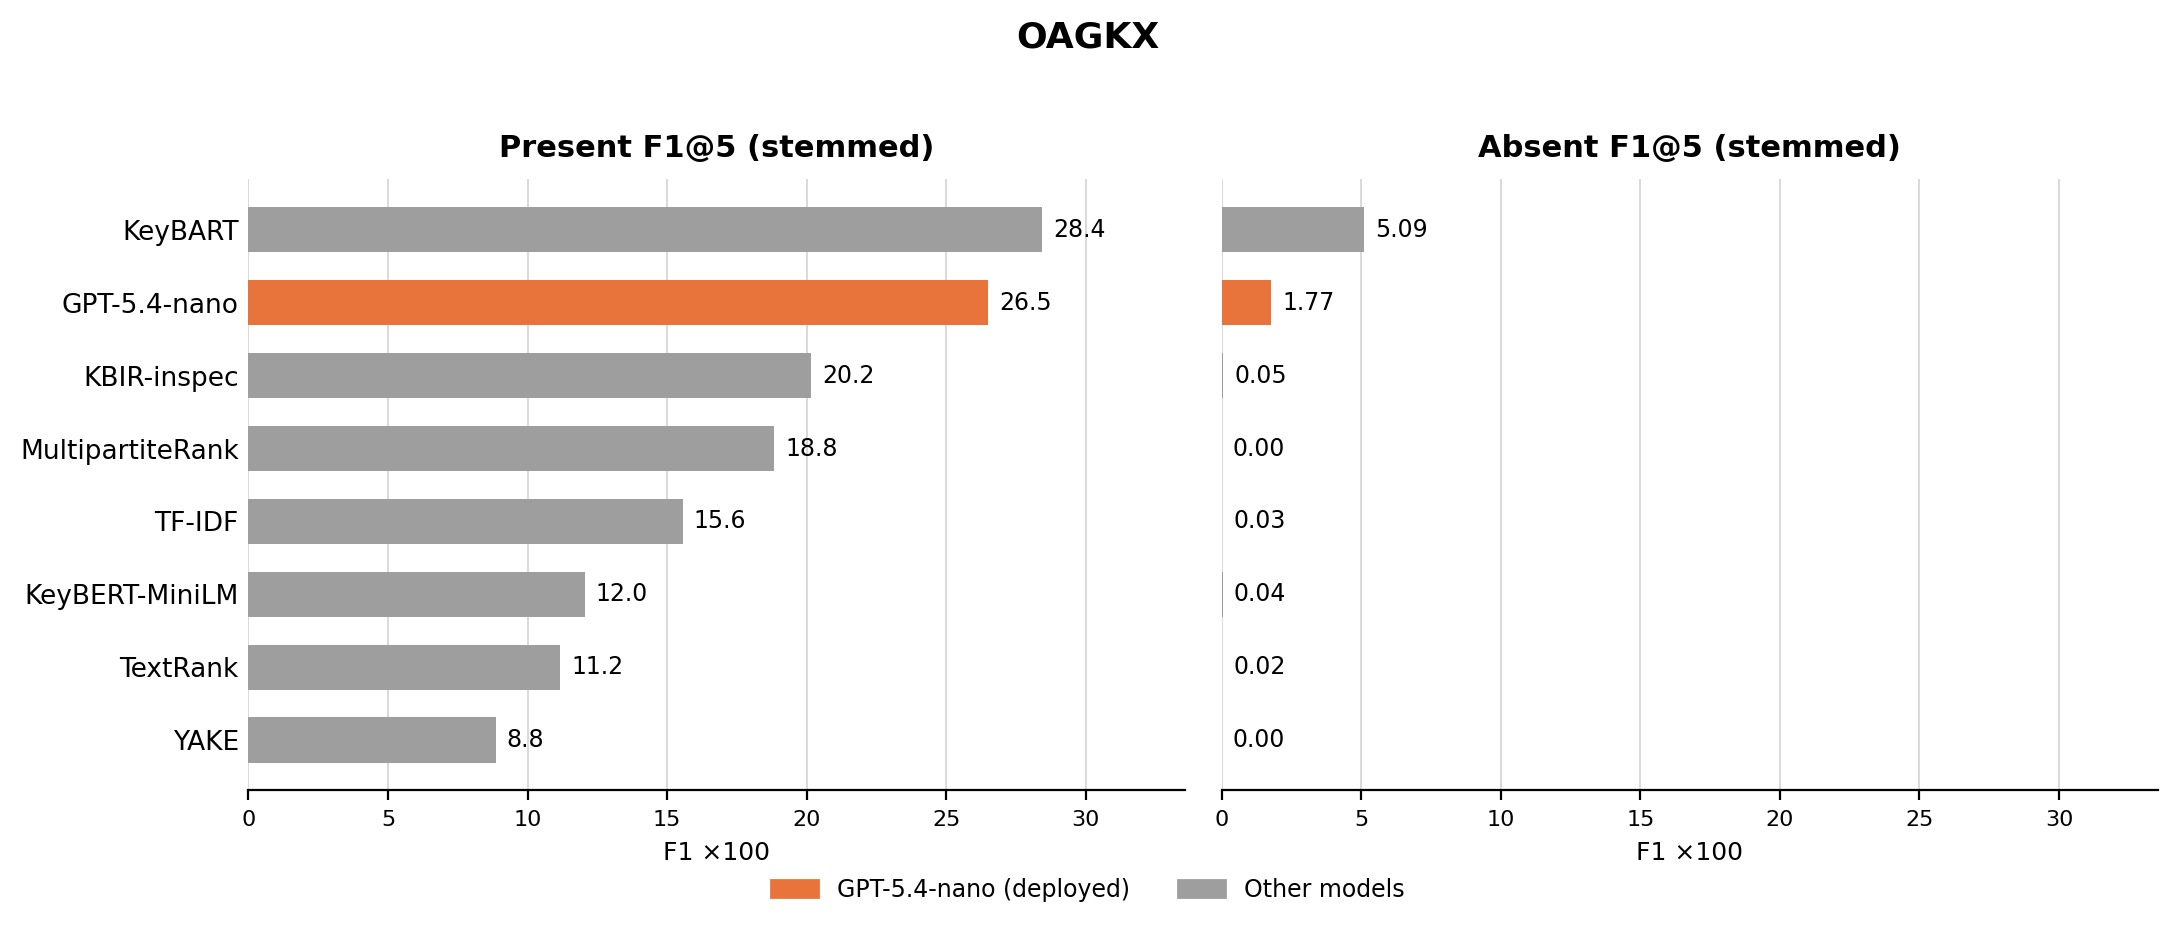
\includegraphics[width=\textwidth]{images/data_and_results/keyword_oagkx.png}
\caption{OAGKX keyword extraction, present and absent F1@5 by model with stemming. The deployed model GPT-5.4-nano is shown in orange and the remaining baselines in grey.}
\label{fig:kw-oagkx}
\end{figure*}

\begin{table}[t]
\caption{PubMedAKE keyword extraction, present and absent F1@5 with stemming. Models are ordered by present F1, and GPT-5.4-nano is the deployed model.}
\label{tab:kw-pubmedake}
\centering
\footnotesize
\begin{tabular}{@{}lrr@{}}
\toprule
Model & Present F1@5 & Absent F1@5 \\
\midrule
\textbf{GPT-5.4-nano} & \textbf{36.44} & \textbf{1.30} \\
TF-IDF & 24.06 & 0.03 \\
MultipartiteRank & 23.06 & 0.00 \\
KBIR-inspec & 19.36 & 0.01 \\
KeyBART & 18.41 & 1.29 \\
YAKE & 12.92 & 0.01 \\
KeyBERT-MiniLM & 6.78 & 0.01 \\
TextRank & 4.68 & 0.00 \\
\bottomrule
\end{tabular}
\end{table}

\begin{figure*}[t]
\centering
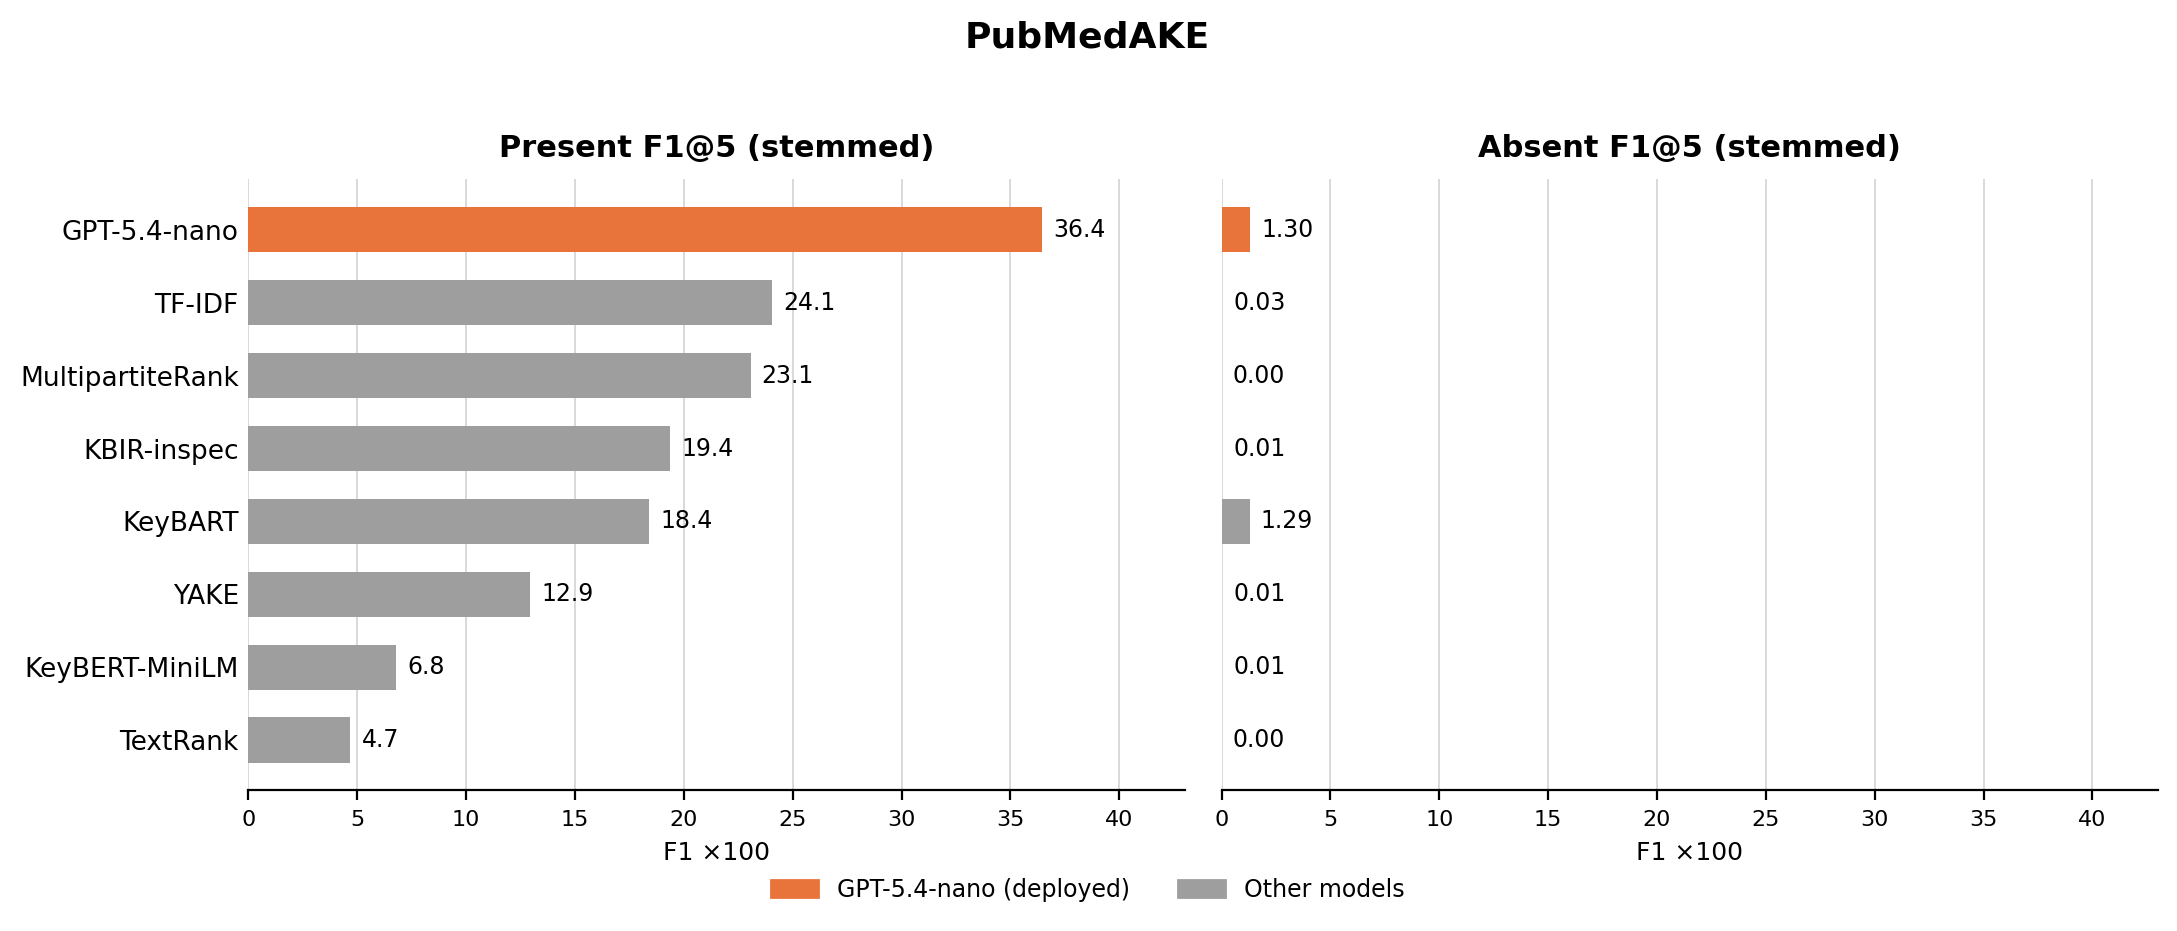
\includegraphics[width=\textwidth]{images/data_and_results/keyword_pubmedake.png}
\caption{PubMedAKE keyword extraction, present and absent F1@5 by model with stemming. The deployed model GPT-5.4-nano is shown in orange and the remaining baselines in grey.}
\label{fig:kw-pubmedake}
\end{figure*}

GPT-5.4-nano was benchmarked for keyword generation against a set of statistical and neural baselines on KPBiomed, OAGKX, and PubMedAKE. Tables~\ref{tab:kw-kpbiomed} to~\ref{tab:kw-pubmedake} report the results for each dataset in turn. Throughout, present (extractive) keyphrases, which occur verbatim in the source text, are distinguished from absent (abstractive) keyphrases, which do not and so must be generated. Matches are scored by F1 at five with light stemming, so that a keyphrase and its stem count as a match while a different word of the same meaning does not.

On the present keyphrase tasks, GPT-5.4-nano records the highest score on KPBiomed and PubMedAKE and the second highest on OAGKX, where KeyBART leads. Its margin is widest on PubMedAKE, at 36.44 against a next-best of 24.06.

On the absent keyphrase tasks, which a model can only score on by producing keyphrases that do not occur in the source text, GPT-5.4-nano scores in the low single digits, from 1.30 on PubMedAKE to 1.95 on KPBiomed. These non-zero scores indicate that the model generates a small portion of its keyphrases rather than extracting all of them. The other generative baseline, KeyBART, behaves similarly and records the highest absent score on KPBiomed and OAGKX. The statistical extractors such as TF-IDF, YAKE, TextRank, and MultipartiteRank remain near zero here, since they return only spans found in the source text and so do not generate at all.

\begin{table}[t]
\caption{Keyword extraction stability for GPT-5.4-nano over three runs on a 2000-document sample.}
\label{tab:kw-stability}
\centering
\footnotesize
\begin{tabular}{@{}p{0.66\columnwidth}r@{}}
\toprule
Quantity & Value \\
\midrule
Set-level Jaccard across runs & 0.73 \\
Present-F1 run-to-run std & $\pm$0.07 \\
Deterministic baselines (TF-IDF, YAKE, TextRank, MultipartiteRank, KeyBERT, KBIR) & 1.00 \\
\bottomrule
\end{tabular}
\end{table}

Table~\ref{tab:kw-stability} reports a reproducibility check for GPT-5.4-nano over three runs on a 2000-document sample. The set-level Jaccard similarity across runs is 0.73, meaning that for a given document around 73 percent of the combined set of keyphrases from any two runs is shared by both, equivalent to roughly one in six keyphrases changing between runs. The model is therefore largely repeatable but not deterministic, unlike the baselines, which are reproducible by construction. The effect on measured performance is negligible, with a run-to-run present-F1 standard deviation of 0.07. The same sample also reproduces the full-split figures to within roughly a tenth of a point, confirming that the smaller stability sample does not shift the headline results.

% ----------------------------------------------------------------------------
\subsection{IR Extraction}

\begin{table*}[t]
\caption{Natural-language-to-IR accuracy by model. Joint IR accuracy counts a query as correct when both its entities and its boolean expression are correct under exact matching, reported in the as-deployed or best configuration for each model.}
\label{tab:ir-accuracy}
\centering
\footnotesize
\begin{tabular}{@{}lllcc@{}}
\toprule
Model & Host & Configuration & IR accuracy & 95\% CI \\
\midrule
\textbf{gpt-5.4-nano} & Azure & default, 0 reasoning tok & \textbf{0.937}$^{\dagger}$ & [0.897, 0.983] \\
gpt-5-mini & Azure & default, 384 reasoning tok & 0.931 & [0.879, 0.974] \\
qwen3:8b & Local (Q4) & single-shot & 0.802 & [0.733, 0.871] \\
qwen3:4b & Local (Q4) & thinking$^{\ddagger}$ & 0.784 & [0.707, 0.862] \\
qwen2.5:3b & Local (Q4) & non-reasoning & 0.207 & [0.138, 0.284] \\
phi4-mini & Local (Q4) & non-reasoning & 0.052 & [0.017, 0.095] \\
llama3.2:3b & Local (Q4) & non-reasoning & 0.026 & [0.000, 0.060] \\
\bottomrule
\end{tabular}

\vspace{3pt}
\begin{minipage}{\linewidth}
\footnotesize\itshape
Confidence intervals are 95 percent bootstrap over 1000 iterations. Cross-model gaps that fall within these intervals are treated as ties, and bold marks the deployed model. The dagger denotes a three-run mean, whose single-run range is 0.914 to 0.940, with temperature zero returning a byte-identical output on 96.6 percent of queries (Table~\ref{tab:ir-stability}). The double dagger denotes qwen3:4b, whose single-shot configuration produced degenerate empty output, so its thinking configuration is its only usable score.
\end{minipage}
\end{table*}

\begin{figure}[t]
\centering
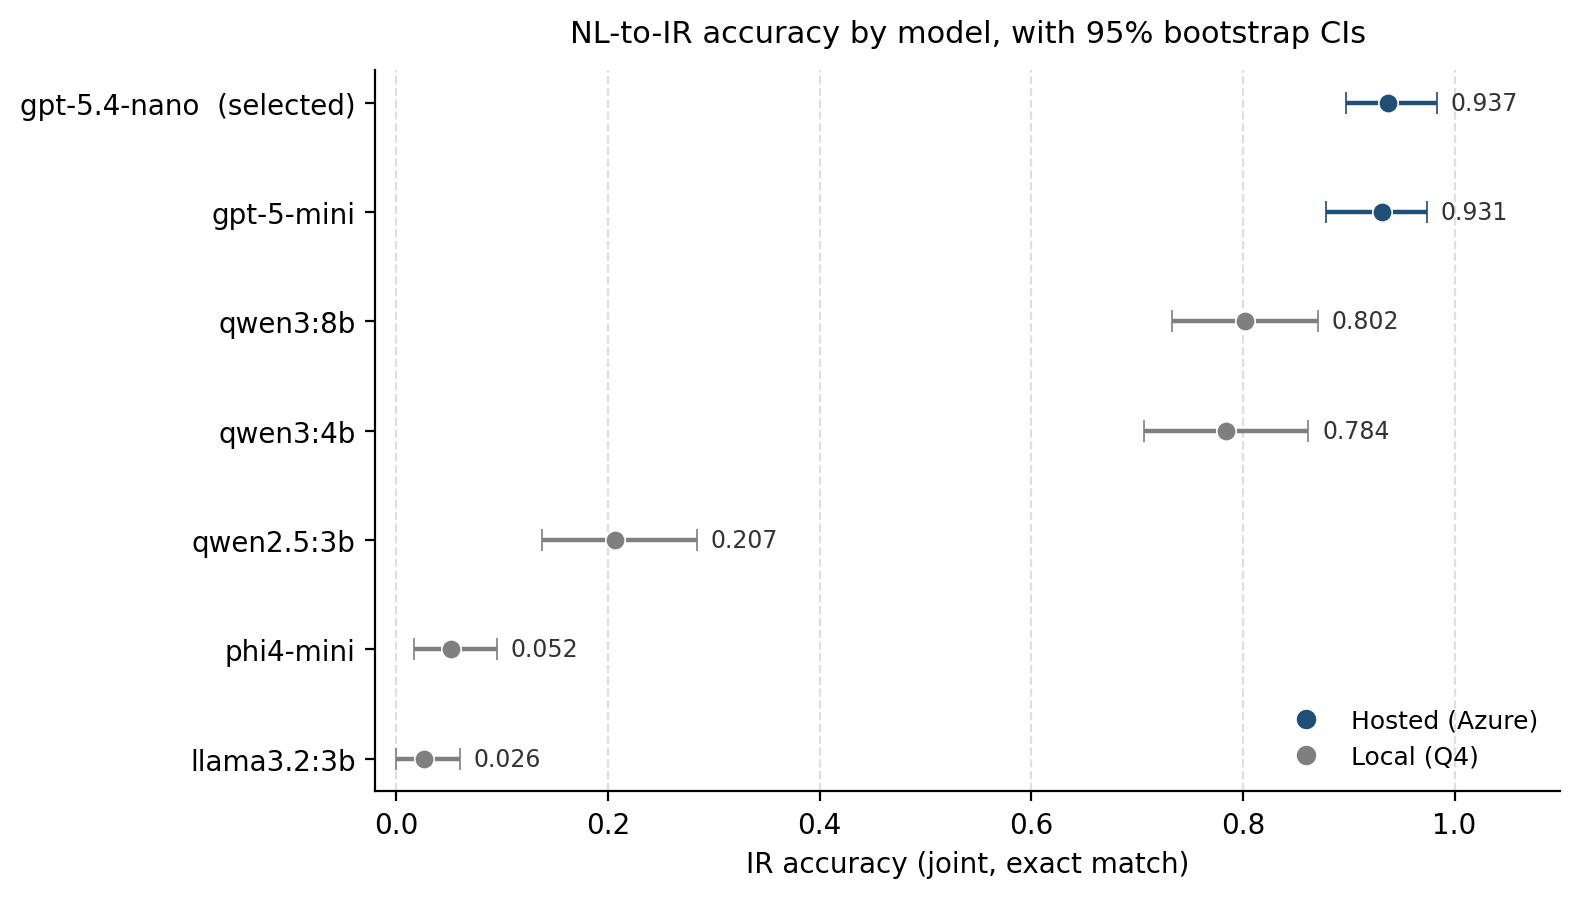
\includegraphics[width=\columnwidth]{images/data_and_results/ir_accuracy_ci.png}
\caption{Natural-language-to-IR joint accuracy by model on the hand-built gold set, with 95 percent bootstrap confidence intervals from 1000 resamples.}
\label{fig:ir-accuracy}
\end{figure}

GPT-5.4-nano was benchmarked for natural-language-to-IR extraction against a set of hosted and local models on a hand-built gold set of queries paired with their correct intermediate representations. The set was constructed to exercise every entity type the system supports across a range of boolean structures, from single topics through to bracketed combinations of AND, OR, and NOT, so that performance on it reflects the input and output behaviour the system actually requires. The headline measure, IR accuracy, is the joint figure reported in Table~\ref{tab:ir-accuracy}, counting a query as correct only when both its extracted entities and its boolean expression are correct under exact matching.

Figure~\ref{fig:ir-accuracy} plots each model's accuracy with its 95 percent bootstrap interval. The two hosted models lead the benchmark by a clear margin, with GPT-5.4-nano highest at an IR accuracy of 0.937 and GPT-5-mini close behind at 0.931. Both hosted intervals clear those of every local model without overlap, placing the hosted advantage beyond sampling noise, while the two overlap each other and are statistically indistinguishable. Among the local models, the two strongest (qwen3:8b and qwen3:4b) reach around 0.80, and the three smaller models fall away sharply to 0.207, 0.052, and 0.026, near the floor of the task.

\begin{table}[t]
\caption{Effect of reasoning on IR accuracy.}
\label{tab:ir-reasoning}
\centering
\footnotesize
\begin{tabular}{@{}lccc@{}}
\toprule
Model & Reasoning off & Reasoning on & $\Delta$ \\
\midrule
gpt-5.4-nano & 0.914 & 0.922 & +0.008 \\
gpt-5-mini & \textbf{0.750} & \textbf{0.940} & \textbf{+0.190} \\
\bottomrule
\end{tabular}

\vspace{3pt}
\begin{minipage}{\linewidth}
\footnotesize\itshape
Reasoning is controlled through the Azure \texttt{reasoning\_effort} setting with tokens accounted. Reasoning on used approximately 246 tokens per query for gpt-5.4-nano and 896 for gpt-5-mini, while reasoning off used none. Reasoning lifts the weaker model in each tier, while the stronger one is already at its ceiling.
\end{minipage}
\end{table}

Table~\ref{tab:ir-reasoning} isolates the effect of reasoning on the two GPT models. GPT-5.4-nano gains almost nothing from it, moving from 0.914 without reasoning to 0.922 with around 246 reasoning tokens, a difference of 0.008, and so reaches its accuracy in a single pass with no reasoning budget. GPT-5-mini behaves differently, scoring only 0.750 without reasoning and rising to 0.940 once reasoning is enabled, at a cost of around 896 reasoning tokens per query. The stronger model is already at its ceiling unaided, whereas the weaker one becomes competitive only by spending a substantial token budget.

\begin{table}[t]
\caption{Deployed model, metric decomposition in the default-effort configuration.}
\label{tab:ir-decomp}
\centering
\footnotesize
\begin{tabular}{@{}lcc@{}}
\toprule
Metric & Value & 95\% CI \\
\midrule
IR accuracy (joint) & 0.937 & [0.897, 0.983] \\
Entity F1 (micro) & 0.984 & [0.969, 0.995] \\
Entity F1 (macro) & 0.982 & [0.967, 0.994] \\
Expression equivalence & 0.931 & [0.888, 0.974] \\
Expression graded & 0.985 & [0.974, 0.995] \\
\bottomrule
\end{tabular}

\vspace{3pt}
\begin{minipage}{\linewidth}
\footnotesize\itshape
Joint accuracy is bounded by expression equivalence, since entity extraction almost never fails on its own.
\end{minipage}
\end{table}

\begin{table}[t]
\caption{Deployed model, accuracy by stratum, ordered hardest first.}
\label{tab:ir-stratum}
\centering
\footnotesize
\begin{tabular}{@{}lrrr@{}}
\toprule
Stratum & $n$ & IR accuracy & failures \\
\midrule
\texttt{filter\_distractor} & 10 & 0.700 & 3 \\
\texttt{multi\_negation} & 10 & 0.800 & 2 \\
\texttt{deep\_nested} & 12 & 0.833 & 2 \\
\texttt{hard\_typing} & 12 & 0.917 & 1 \\
\texttt{single\_concept} & 6 & 1.000 & 0 \\
\texttt{multi\_concept} & 12 & 1.000 & 0 \\
\texttt{exclusion} & 12 & 1.000 & 0 \\
\texttt{nested} & 12 & 1.000 & 0 \\
\texttt{mixed\_entity} & 16 & 1.000 & 0 \\
\texttt{review\_style} & 14 & 1.000 & 0 \\
\bottomrule
\end{tabular}

\vspace{3pt}
\begin{minipage}{\linewidth}
\footnotesize\itshape
The count $n$ is small per stratum, at sixteen or fewer, so the failure counts are a more reliable read than the rate, and the per-stratum 95 percent intervals are wide, for example \texttt{filter\_distractor} at 0.700 is seven of ten.
\end{minipage}
\end{table}

Tables~\ref{tab:ir-decomp} and~\ref{tab:ir-stratum} decompose the chosen model's performance, which is strong across both components and most query types. By component, entity extraction is near-perfect, with a micro F1 of 0.984 and a macro F1 of 0.982, while expression equivalence is lower at 0.931 (a graded variant that credits partially correct expressions reaches 0.985). The joint IR accuracy of 0.937 is therefore bounded by the expression score, since entity extraction almost never fails on its own. By query type, the model is perfect on six of the ten strata, covering single and multiple concepts, exclusions, nesting, mixed entities, and review-style queries. Its errors concentrate in the remaining four. The largest source is \texttt{filter\_distractor}, where three of ten queries fail because the model miscategorises a filter term such as a year or citation bound as a searchable entity. The rest fall on the structurally hardest queries, with two of ten failing on multiple negations, two of twelve on deep nesting, and one of twelve on hard typing. Per-stratum counts are small, at sixteen queries or fewer, so the failure counts are a more reliable read than the rates.

\begin{table}[t]
\caption{Stability of the deployed model over three runs.}
\label{tab:ir-stability}
\centering
\footnotesize
\begin{tabular}{@{}p{0.46\columnwidth}cc@{}}
\toprule
Metric & temp 0 & temp 0.7 \\
\midrule
IR identical across all 3 runs & 0.966 & 0.957 \\
Run-to-run IR-accuracy std & 0.004 & 0.004 \\
Majority-vote@3 vs single run & 0.931 vs 0.940 & 0.940 vs 0.940 \\
\bottomrule
\end{tabular}

\vspace{3pt}
\begin{minipage}{\linewidth}
\footnotesize\itshape
Temperature zero is highly but not perfectly deterministic, and majority voting adds nothing.
\end{minipage}
\end{table}

Table~\ref{tab:ir-stability} reports a stability check over three runs. Although GPT-5.4-nano is not deterministic, at temperature zero it returns an identical IR on 96.6 percent of queries, with a run-to-run accuracy standard deviation of 0.004. Aggregating three runs by majority vote changes nothing, at 0.931 against 0.940 for a single run, so the three-run mean of 0.937 reported in Table~\ref{tab:ir-accuracy} is used throughout.

% ----------------------------------------------------------------------------
\subsection{Dense Bi-encoder Retrieval}

\begin{table*}[t]
\caption{Dense bi-encoder retrieval on SciRepEval ad-hoc search, nDCG $\times$100 with 95 percent bootstrap confidence intervals.}
\label{tab:bienc-results}
\centering
\scriptsize
\setlength{\tabcolsep}{4pt}
\begin{tabular}{@{}p{3.0cm}llll@{}}
\toprule
Model & NFCorpus & TREC-CoVID & Search & Average \\
\midrule
Qwen3-Embedding-4B (int8) & \textbf{80.02 [77.75, 82.17]} & \textbf{94.28 [92.96, 95.43]} & 75.54 [74.93, 76.17] & \textbf{83.28 [82.35, 84.19]} \\
EmbeddingGemma-300M & 79.13 [76.84, 81.29] & 92.45 [90.68, 94.03] & 75.32 [74.66, 75.93] & 82.30 [81.32, 83.31] \\
Qwen3-Embedding-0.6B & 77.94 [75.75, 80.22] & 93.90 [92.52, 95.10] & 75.03 [74.41, 75.65] & 82.29 [81.32, 83.25] \\
text-embedding-3-small (existing) & 78.78 [76.61, 81.05] & 92.38 [90.58, 93.96] & 75.14 [74.52, 75.74] & 82.10 [81.08, 83.05] \\
mxbai-embed-large-v1 & 79.37 [77.19, 81.72] & 91.77 [90.02, 93.25] & 74.92 [74.29, 75.56] & 82.02 [81.06, 82.96] \\
SPECTER2-adhoc-query & 70.46 [68.01, 72.97] & 90.08 [87.84, 92.13] & \textbf{78.22 [77.60, 78.86]} & 79.59 [78.46, 80.71] \\
BGE-M3 & 74.05 [71.72, 76.35] & 89.21 [87.08, 91.16] & 74.82 [74.20, 75.46] & 79.36 [78.29, 80.42] \\
SPECTER2-base (existing) & 72.03 [69.60, 74.54] & 89.46 [86.99, 91.58] & 73.76 [73.12, 74.41] & 78.42 [77.27, 79.58] \\
\bottomrule
\end{tabular}

\vspace{3pt}
\begin{minipage}{\linewidth}
\footnotesize\itshape
The metric is SciRepEval ad-hoc-search full-ranking nDCG over a per-query candidate pool, not BEIR full-corpus nDCG@10. Confidence intervals are 95 percent bootstrap [lo, hi] over 1000 iterations with seed 42, and bold marks the best point estimate per column. On Average the top five models' intervals overlap, a statistical tie, and SPECTER2-adhoc-query's Search lead is the one between-model gap whose interval clears the general models.
\end{minipage}
\end{table*}

\begin{figure}[t]
\centering
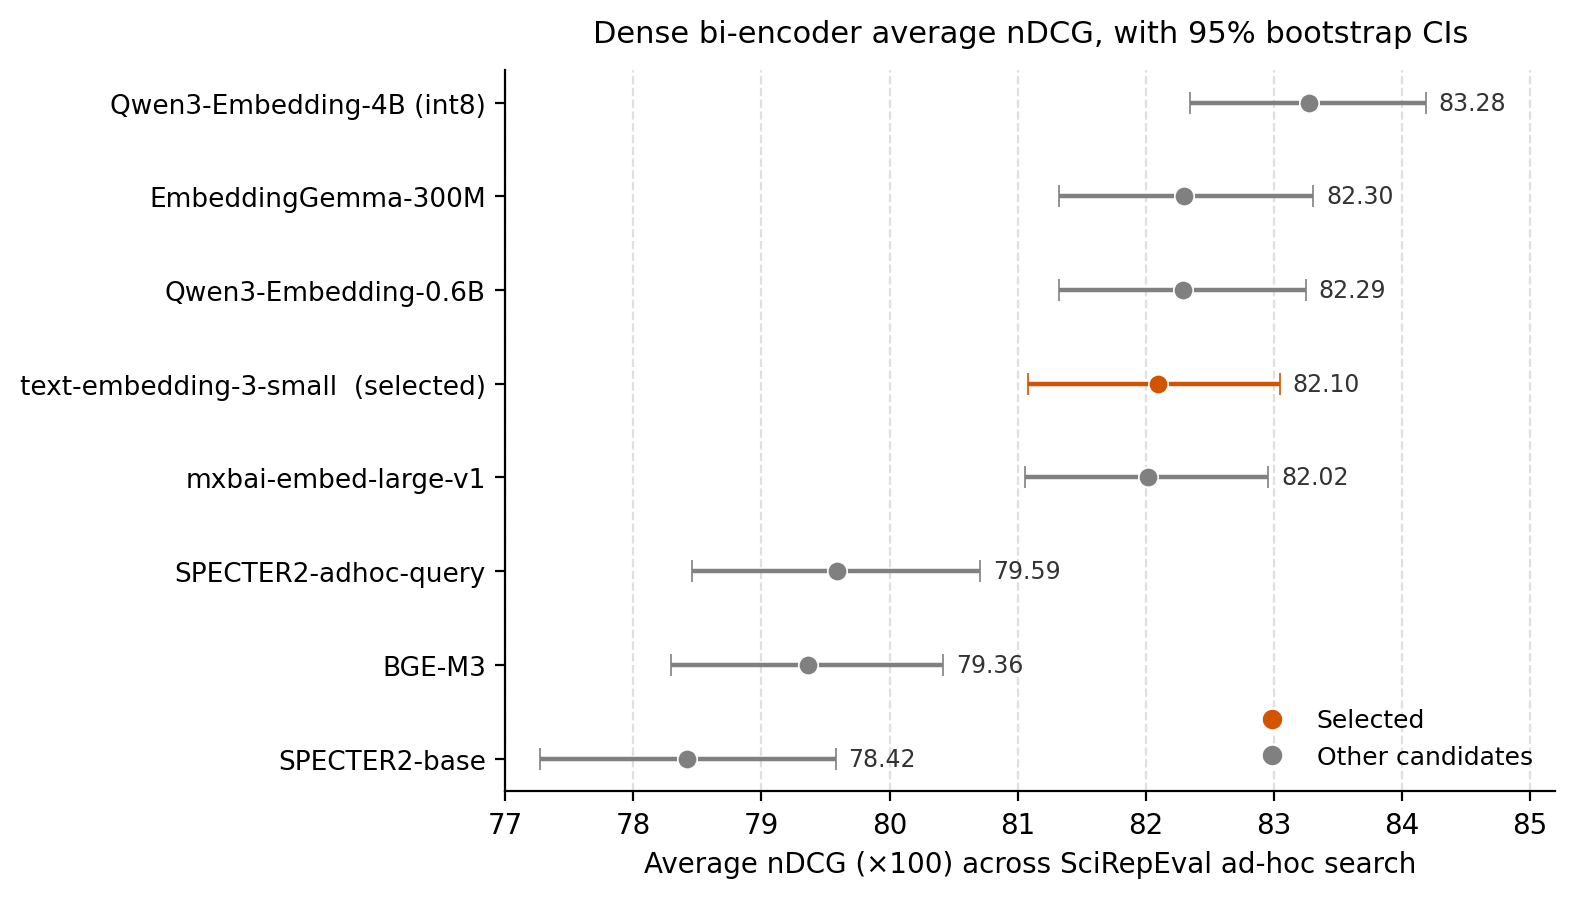
\includegraphics[width=\columnwidth]{images/data_and_results/biencoder_average.png}
\caption{Dense bi-encoder average nDCG across the three SciRepEval ad-hoc search tasks, with 95 percent bootstrap confidence intervals from 1000 resamples. The selected model is shown in orange.}
\label{fig:bienc-avg}
\end{figure}

\begin{figure}[t]
\centering
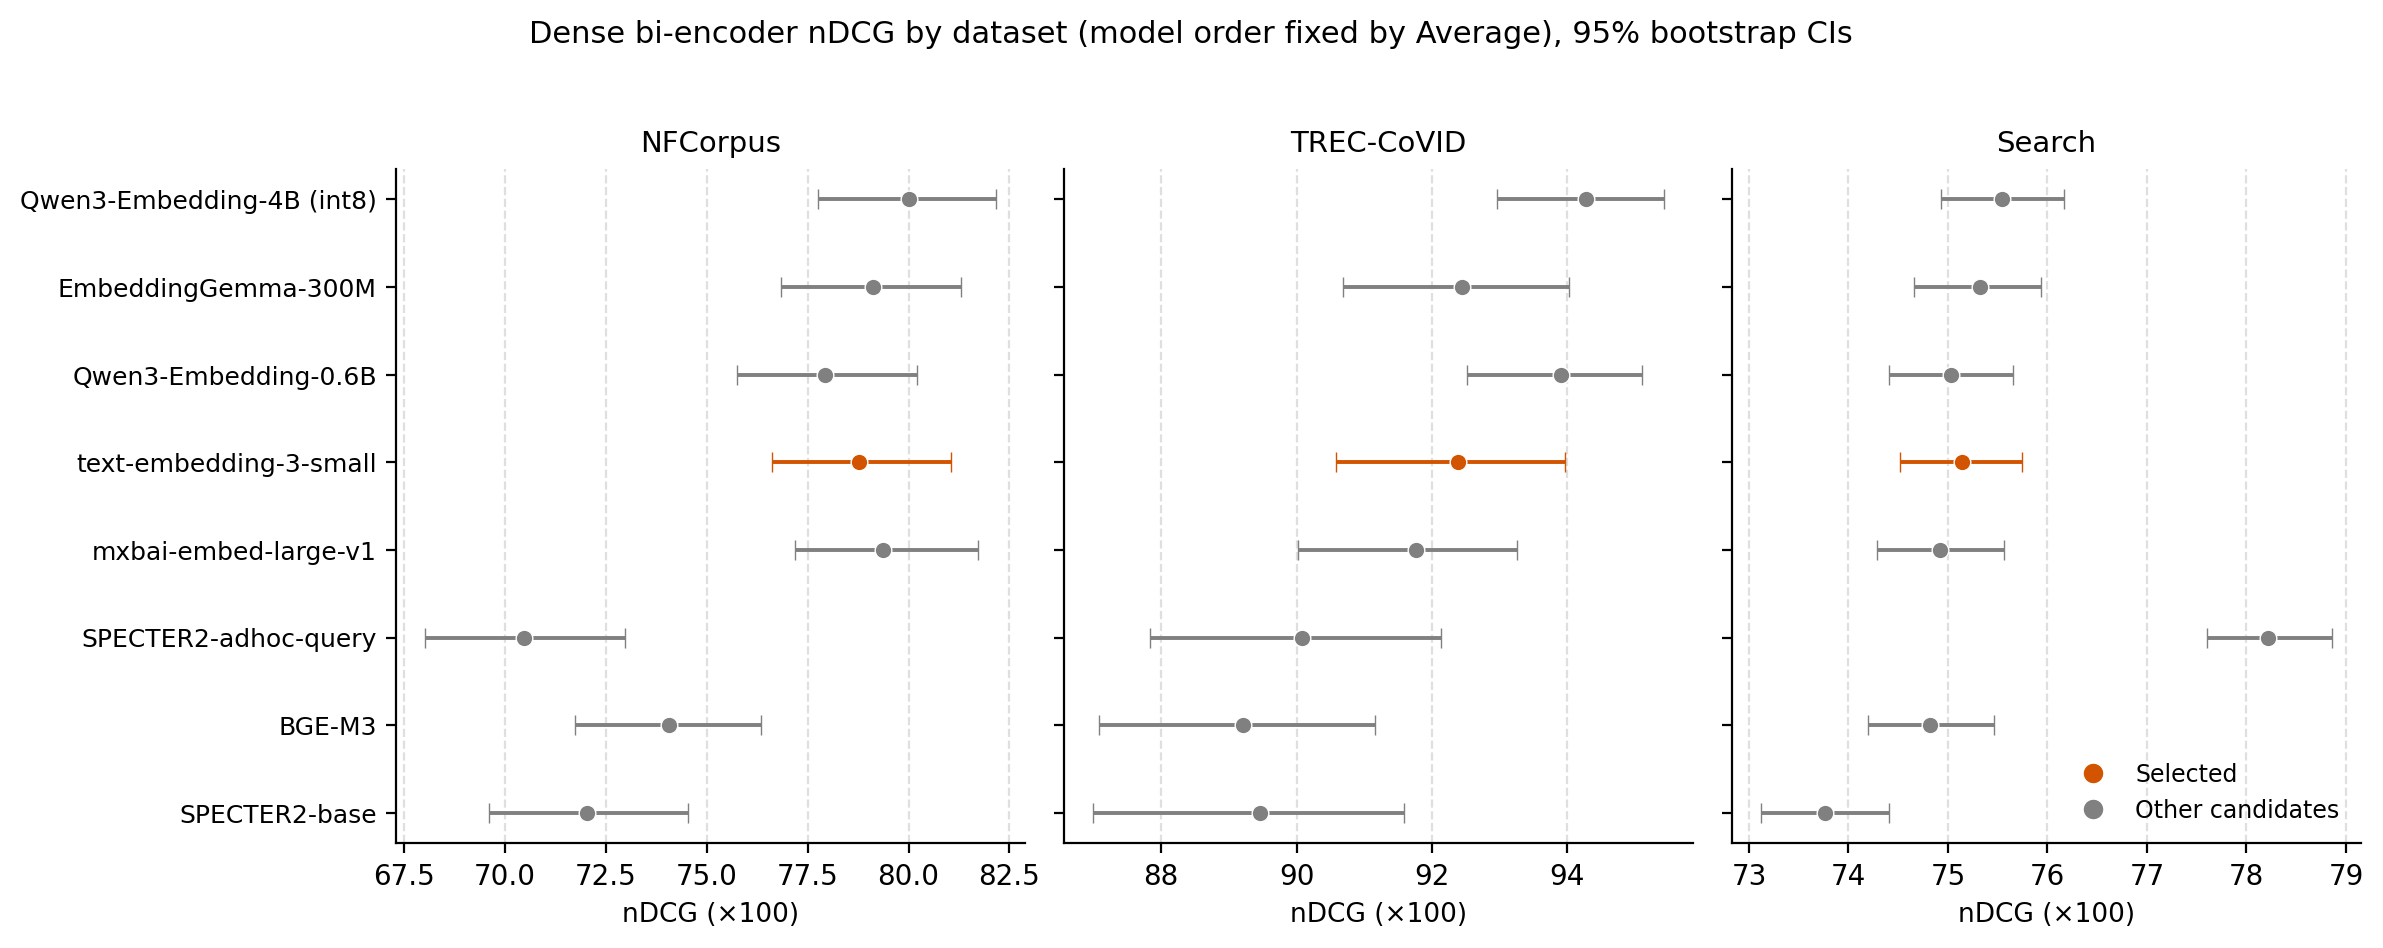
\includegraphics[width=\columnwidth]{images/data_and_results/biencoder_by_dataset.png}
\caption{Dense bi-encoder nDCG on each SciRepEval ad-hoc search task, with models held in their Average order for comparison and 95 percent bootstrap confidence intervals. The selected model is shown in orange.}
\label{fig:bienc-pertask}
\end{figure}

text-embedding-3-small was selected as the dense bi-encoder. The candidate models were evaluated on the three ad-hoc search tasks of SciRepEval, namely NFCorpus, TREC-CoVID, and Search, scored by nDCG. The figure reported is SciRepEval full-ranking nDCG over a per-query candidate pool rather than BEIR full-corpus nDCG@10, which keeps the stage comparable to the scientific retrieval benchmark established in Section~II-D. All scores are nDCG $\times$100 with 95 percent bootstrap intervals from 1000 resamples.

Table~\ref{tab:bienc-results} reports the per-task and average scores in full, and Figure~\ref{fig:bienc-avg} plots each model's average nDCG with its interval. The selected model records an average of 82.10. Qwen3-Embedding-4B holds the highest point estimate at 83.28, but the intervals of the top five models all overlap, forming a statistical tie that contains text-embedding-3-small along with EmbeddingGemma-300M, Qwen3-Embedding-0.6B, and mxbai-embed-large-v1. A clear margin separates this group from the lower three, SPECTER2-adhoc-query at 79.59, BGE-M3 at 79.36, and SPECTER2-base at 78.42, whose intervals fall below the leading cluster.

The average conceals a difference in where each model does its work, shown per task in Figure~\ref{fig:bienc-pertask}. On NFCorpus and TREC-CoVID the general-purpose embedders lead, with Qwen3-Embedding-4B highest on both. On Search the order changes. SPECTER2-adhoc-query scores 78.22 against a field clustered near 75, and this is the single between-model gap on any one task whose interval clears the general models. The same model is weakest on NFCorpus at 70.46, so its Search lead does not survive into the average. The selected model sits within the leading group on each of the three tasks.

\begin{table*}[t]
\caption{Deployment characteristics of the candidate bi-encoders.}
\label{tab:bienc-deploy}
\centering
\footnotesize
\begin{tabular}{@{}lllll@{}}
\toprule
Model & Params (approx.) & Embedding dim & Precision & Self-hostable \\
\midrule
Qwen3-Embedding-4B & $\sim$4 B & 2560 & int8 & yes \\
EmbeddingGemma-300M & $\sim$300 M & 768 & fp16 & yes \\
Qwen3-Embedding-0.6B & $\sim$0.6 B & 1024 & fp16 & yes \\
text-embedding-3-small & undisclosed & 1536 & n/a & no (paid API) \\
mxbai-embed-large-v1 & $\sim$335 M & 1024 & fp16 & yes \\
SPECTER2-adhoc-query & $\sim$110 M & 768 & fp16 & yes \\
BGE-M3 & $\sim$568 M & 1024 & fp16 & yes \\
SPECTER2-base & $\sim$110 M & 768 & fp16 & yes \\
\bottomrule
\end{tabular}

\vspace{3pt}
\begin{minipage}{\linewidth}
\footnotesize\itshape
In-memory footprint per stored vector scales with embedding dimension at int8, at roughly one byte per dimension, giving around 65 GB at 768 dimensions, 87 GB at 1024, 131 GB at 1536, and 218 GB at 2560 over the 85 million works. Encoding cost scales with parameter count.
\end{minipage}
\end{table*}

Table~\ref{tab:bienc-deploy} records the deployment characteristics that the nDCG scores do not, namely approximate parameter count, embedding dimension, precision, and whether the model is self-hostable. In-memory footprint per stored vector scales with embedding dimension at int8, from around 65 GB at 768 dimensions to around 218 GB at 2560 dimensions over the 85 million works, while encoding cost scales with parameter count. The selected model has an embedding dimension of 1536, placing its footprint at around 131 GB, and is served through a paid API rather than self-hosted.

% ----------------------------------------------------------------------------
\subsection{Cross-encoder Re-ranking}

\begin{table*}[t]
\caption{Cross-encoder re-ranking on SciRepEval ad-hoc search, nDCG $\times$100 with 95 percent bootstrap confidence intervals, sorted by Average.}
\label{tab:xenc-results}
\centering
\scriptsize
\setlength{\tabcolsep}{4pt}
\begin{tabular}{@{}p{3.2cm}llll@{}}
\toprule
Model (scorer) & NFCorpus & TREC-CoVID & Search & Average \\
\midrule
Cohere Rerank 4.0 Pro (API) & \textbf{80.42 [78.17, 82.60]} & \textbf{94.60 [93.30, 95.71]} & 75.39 [74.76, 76.00] & \textbf{83.47 [82.54, 84.33]} \\
Qwen3-Reranker-4B (int8) & 80.10 [77.94, 82.14] & 94.37 [92.90, 95.60] & 74.93 [74.32, 75.56] & 83.13 [82.18, 83.99] \\
Cohere Rerank 4.0 Fast (API) & 78.77 [76.55, 80.98] & 94.15 [92.83, 95.31] & \textbf{75.42 [74.75, 76.04]} & 82.78 [81.83, 83.68] \\
Qwen3-Reranker-0.6B (fp16) & 78.06 [75.65, 80.24] & 93.98 [92.59, 95.20] & 75.25 [74.59, 75.85] & 82.43 [81.50, 83.34] \\
mxbai-rerank-large-v1 (435M) & 78.32 [76.08, 80.76] & 91.50 [89.43, 93.33] & 74.78 [74.15, 75.46] & 81.53 [80.48, 82.59] \\
jina-reranker-v2-base (278M) & 76.73 [74.49, 79.01] & 91.84 [90.05, 93.52] & 75.37 [74.73, 75.99] & 81.31 [80.28, 82.30] \\
MedCPT-Cross-Encoder (109M, biomed) & 75.70 [73.21, 78.03] & 88.91 [86.61, 90.97] & 73.97 [73.34, 74.63] & 79.53 [78.40, 80.66] \\
ms-marco-MiniLM-L-6-v2 (22M) & 73.10 [70.78, 75.48] & 88.78 [86.41, 90.90] & 75.21 [74.58, 75.84] & 79.03 [77.90, 80.13] \\
bge-reranker-v2-m3 (568M) & 70.71 [68.31, 73.07] & 90.30 [88.29, 92.18] & 74.40 [73.78, 75.05] & 78.47 [77.37, 79.53] \\
ms-marco-MiniLM-L-12-v2 (33M) & 69.88 [67.41, 72.38] & 87.17 [84.73, 89.52] & 75.09 [74.44, 75.71] & 77.38 [76.17, 78.54] \\
bge-reranker-large (560M) & 66.49 [64.11, 68.85] & 87.27 [84.61, 89.62] & 74.22 [73.59, 74.85] & 76.00 [74.80, 77.16] \\
bge-reranker-base (278M) & 58.75 [56.38, 60.94] & 84.98 [82.12, 87.60] & 72.60 [71.97, 73.24] & 72.11 [70.84, 73.35] \\
gte-reranker-modernbert-base (150M) & 48.88 [46.82, 50.93] & 79.03 [76.40, 81.60] & 69.94 [69.26, 70.60] & 65.95 [64.91, 67.07] \\
\bottomrule
\end{tabular}

\vspace{3pt}
\begin{minipage}{\linewidth}
\footnotesize\itshape
The metric is SciRepEval ad-hoc-search full-ranking nDCG over a reranking pool, not BEIR full-corpus nDCG@10. Confidence intervals are 95 percent bootstrap [2.5 percent, 97.5 percent] over 1000 iterations with seed 42, with the Average resampled independently within each dataset. The intervals are tight on Search, which has 2585 queries, and wide on TREC-CoVID, which has 50, and bold marks the best point estimate per column. The top four models, namely Cohere Pro, Qwen3-Reranker-4B, Cohere Fast, and Qwen3-Reranker-0.6B, have heavily overlapping Average intervals and form a statistical tie, within which the best self-hostable model, Qwen3-Reranker-4B at int8, is tied with Cohere Pro. On Search the small candidate pool saturates every reranker at around 75. For reference, the bi-encoder embeddings without intervals give the best embedder Qwen3-Embedding-4B at 83.28 Average, SPECTER2-adhoc-query at 78.22 on Search, which is above every reranker here, and text-embedding-3-small at 82.10 Average.
\end{minipage}
\end{table*}

\begin{figure}[t]
\centering
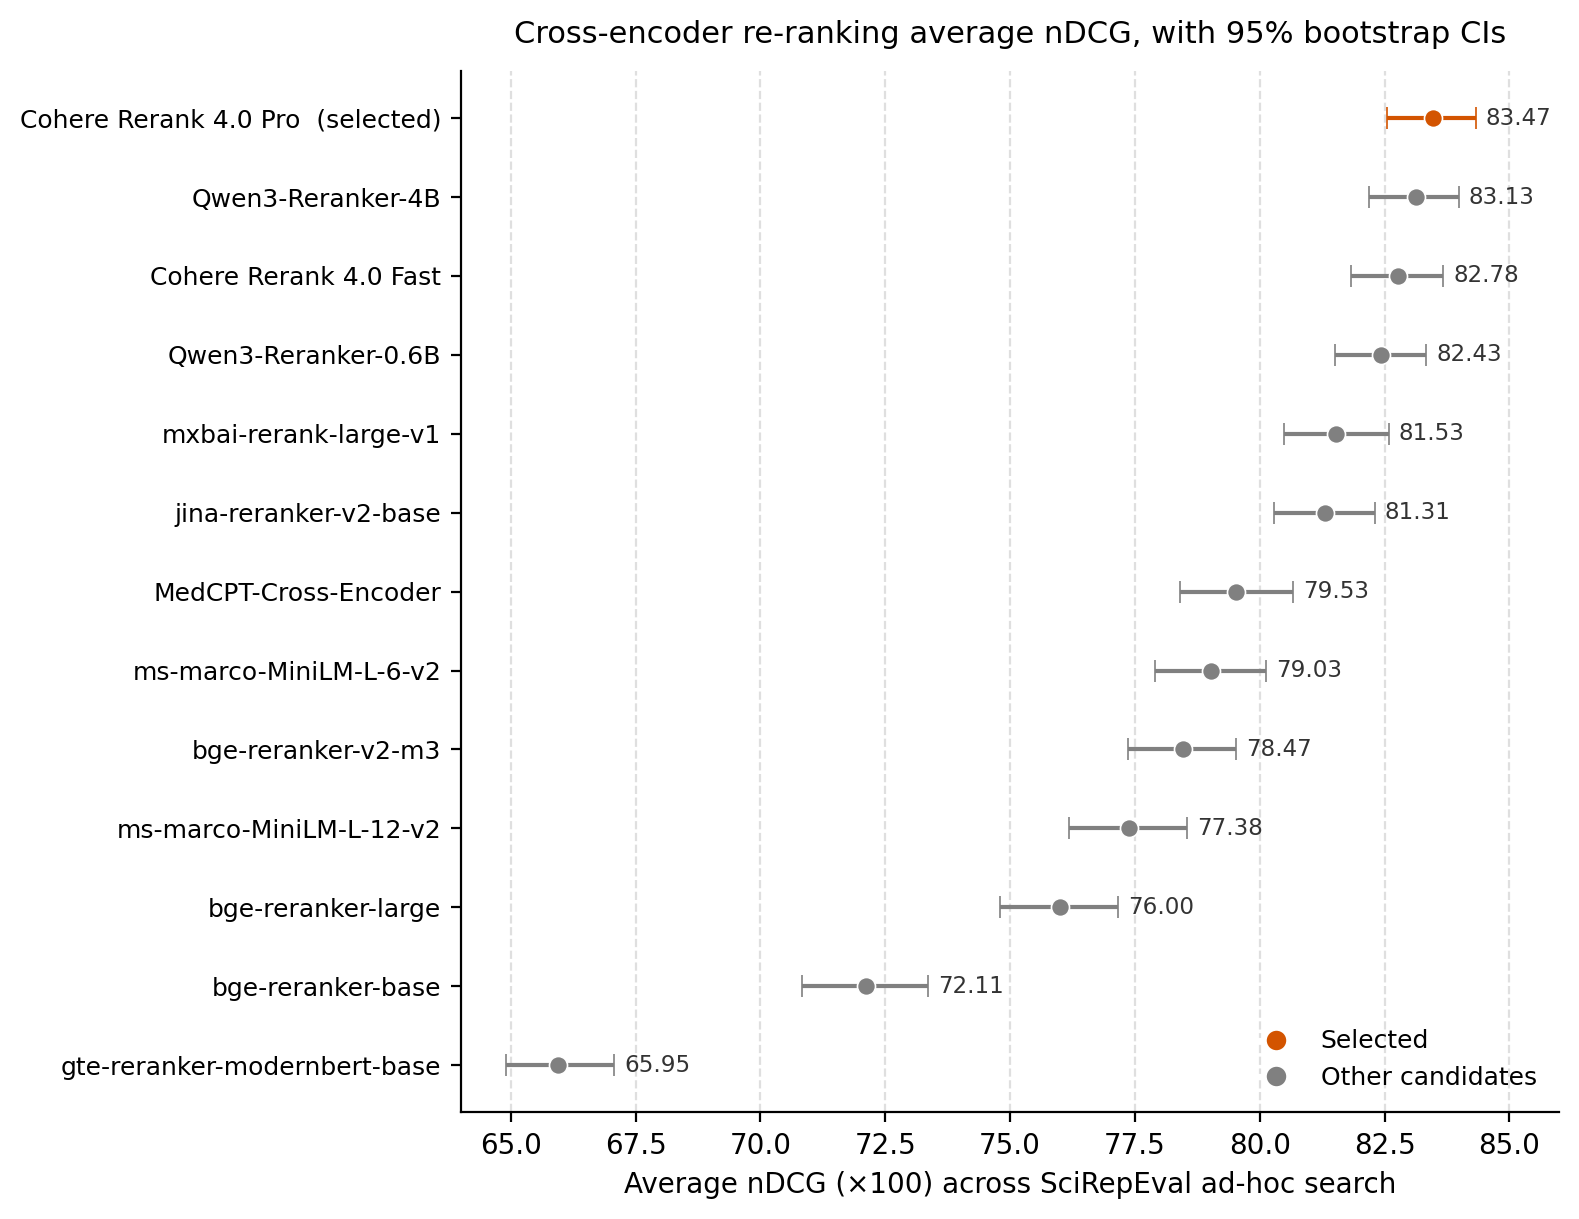
\includegraphics[width=\columnwidth]{images/data_and_results/crossencoder_average.png}
\caption{Cross-encoder re-ranking average nDCG across the three SciRepEval ad-hoc search tasks, with 95 percent bootstrap confidence intervals from 1000 resamples. The selected model is shown in orange.}
\label{fig:xenc-avg}
\end{figure}

\begin{figure}[t]
\centering
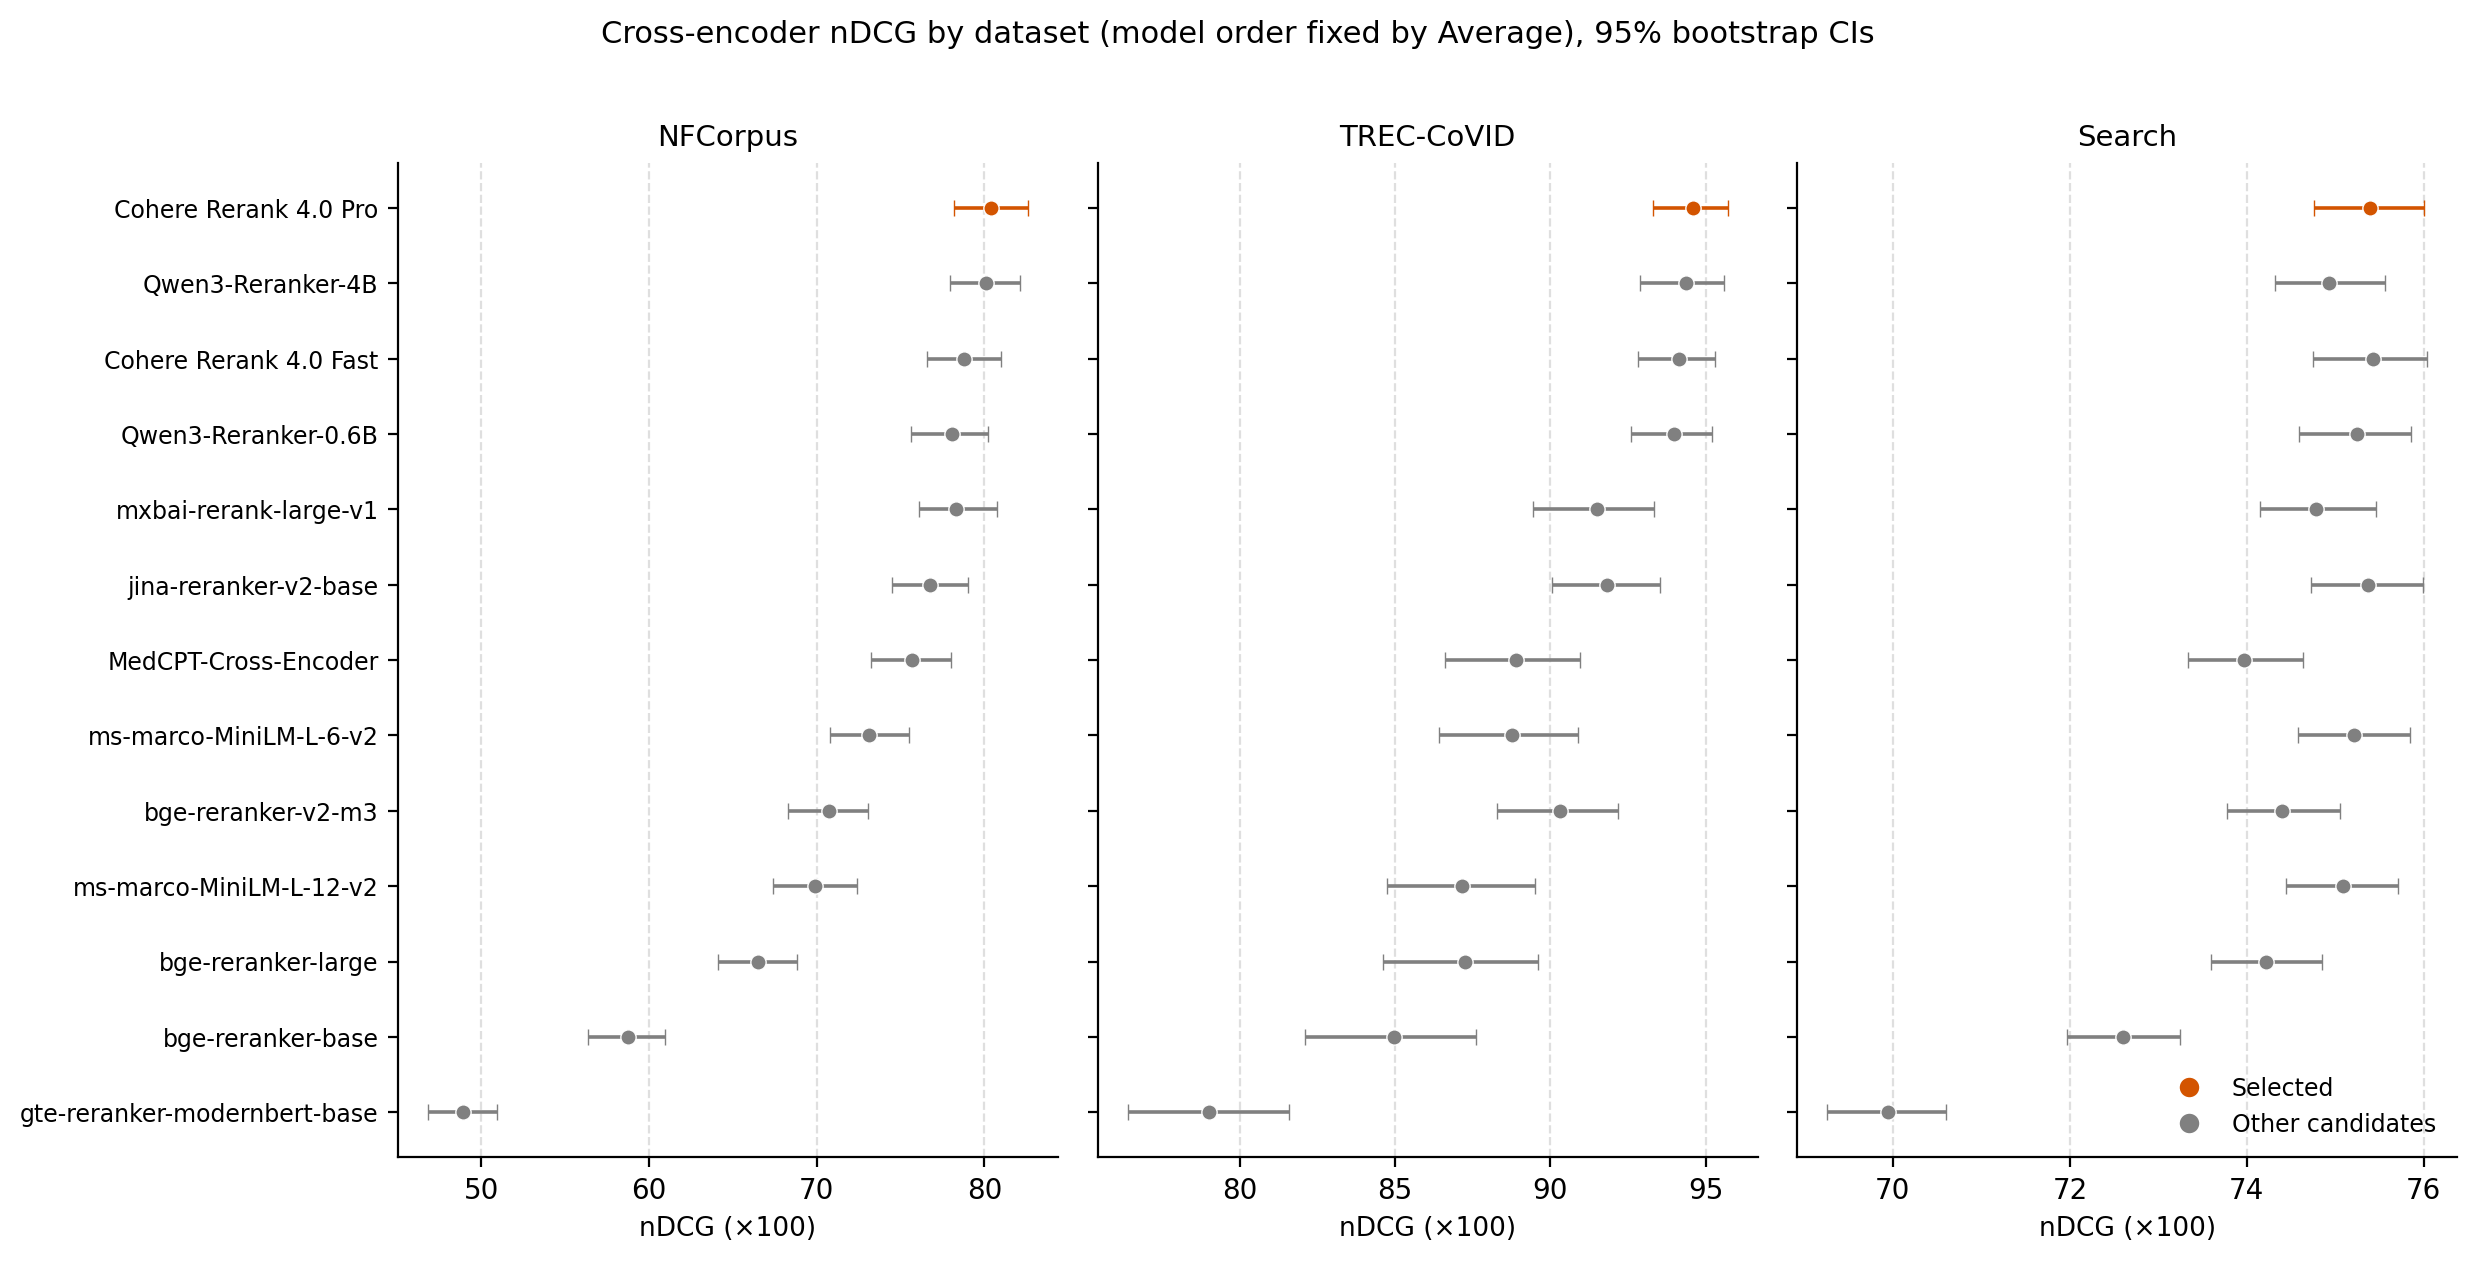
\includegraphics[width=\columnwidth]{images/data_and_results/crossencoder_by_dataset.png}
\caption{Cross-encoder nDCG on each SciRepEval ad-hoc search task, with models held in their Average order for comparison and 95 percent bootstrap confidence intervals. The selected model is shown in orange.}
\label{fig:xenc-pertask}
\end{figure}

Cohere Rerank 4.0 Pro was selected as the cross-encoder. The candidate rerankers were evaluated on the same three SciRepEval ad-hoc search tasks as the bi-encoder and under the same nDCG metric, scoring each model by the ranking it produces when it re-ranks the retrieved candidate pool. All scores are nDCG $\times$100 with 95 percent bootstrap intervals from 1000 resamples. The intervals are tight on Search, which has 2585 queries, and wide on TREC-CoVID, which has 50.

Table~\ref{tab:xenc-results} reports the full per-task and average scores, and Figure~\ref{fig:xenc-avg} plots each model's average with its interval. The selected model holds the highest average at 83.47. Its interval overlaps those of the next three models, Qwen3-Reranker-4B at 83.13, Cohere Rerank 4.0 Fast at 82.78, and Qwen3-Reranker-0.6B at 82.43, so these four form a statistical tie at the top. Within that group the strongest self-hostable model, Qwen3-Reranker-4B, is tied with the selected model. Below the leading four the field descends steadily through a long tail to gte-reranker-modernbert-base at 65.95, a spread of more than seventeen points from top to bottom.

The per-task view in Figure~\ref{fig:xenc-pertask} shows that almost all of this separation comes from NFCorpus, where the models spread across more than thirty points, from 80.42 at the top down to 48.88. Search behaves in the opposite way. Every reranker scores close to 75, since the small candidate pool the stage re-ranks leaves little room to reorder, so the task barely separates the models. TREC-CoVID falls between the two, with a high but noisy spread that reflects its fifty queries.

\begin{table*}[t]
\caption{Deployment characteristics of the candidate cross-encoders.}
\label{tab:xenc-deploy}
\centering
\footnotesize
\begin{tabular}{@{}p{4.5cm}llp{4.0cm}@{}}
\toprule
Model & Params (approx.) & Precision & Self-hostable \\
\midrule
Cohere Rerank 4.0 Pro & undisclosed & n/a & no (paid API) \\
Qwen3-Reranker-4B & $\sim$4 B & int8 & yes (Apache-2.0) \\
Cohere Rerank 4.0 Fast & undisclosed & n/a & no (paid API) \\
Qwen3-Reranker-0.6B & $\sim$0.6 B & fp16 & yes (Apache-2.0) \\
mxbai-rerank-large-v1 & $\sim$435 M & fp16 & yes \\
jina-reranker-v2-base & $\sim$278 M & fp16 & weights CC-BY-NC (non-commercial) \\
MedCPT-Cross-Encoder & $\sim$109 M & fp16 & yes \\
ms-marco-MiniLM-L-6-v2 & $\sim$22 M & fp16 & yes \\
bge-reranker-v2-m3 & $\sim$568 M & fp16 & yes \\
ms-marco-MiniLM-L-12-v2 & $\sim$33 M & fp16 & yes \\
bge-reranker-large & $\sim$560 M & fp16 & yes \\
bge-reranker-base & $\sim$278 M & fp16 & yes \\
gte-reranker-modernbert-base & $\sim$150 M & fp16 & yes \\
\bottomrule
\end{tabular}

\vspace{3pt}
\begin{minipage}{\linewidth}
\footnotesize\itshape
Unlike the bi-encoder, a reranker stores no vectors, so its cost is latency, which scales with parameter count, rather than memory, which is why the stage runs over only around 100 candidates. The Qwen3 rerankers are released under Apache-2.0, while the jina-reranker-v2 weights are CC-BY-NC-4.0 and so are non-commercial and not deployable in a commercial product. The remaining licences should be confirmed against the deployment terms before selection.
\end{minipage}
\end{table*}

Table~\ref{tab:xenc-deploy} records the deployment characteristics, namely approximate parameter count, precision, and whether the model is self-hostable along with its licence. Unlike the bi-encoder, a reranker stores no vectors, so its cost is latency rather than memory and scales with parameter count, which is the reason the stage runs over only around 100 candidates. The self-hostable options carry mixed licences, with the Qwen3 rerankers released under Apache-2.0 and the jina reranker under a non-commercial CC-BY-NC licence, while the selected model is served through a paid API.

% ----------------------------------------------------------------------------
\subsection{Embedding Quantisation}
% Placeholder. Results not yet available.
\textit{[Placeholder. Results comparing int8 against full-precision nDCG, and the resulting accuracy cost, to be added.]}

% ----------------------------------------------------------------------------
\subsection{System-Level Evaluation}
% Placeholder. Results not yet available.
\textit{[Placeholder. End-to-end results over a realistic query set with light relevance judgments to be added.]}

%=======================================================================
% Analysis and Discussion
% Included from main.tex via \input{...} (or \include{...}).
% Contains the section body only: no \documentclass, no \begin{document}.
% Assumes the IEEEtran class already loaded by main.tex (auto A/B/C and
% 1)/2)/3) numbering for \subsection and \subsubsection).
%
% PLACEHOLDERS for Claude Code to reconcile (grep for "PLACEHOLDER"):
%   1. \ref{tab:reasoning-effect} points at the reasoning on/off table
%      (Table X, in the Data and Results section). Its real \label lives
%      in that file; swap this label name for the real one.
%   2. The RQ3 subsection is a stub, pending system-level results.
%
% NOTE: prose mentions of "the system-level evaluation" are intentionally
% left as plain text, not \ref. Convert to refs later if desired.
%=======================================================================

\section{Analysis and Discussion}
\label{sec:analysis-discussion}

\subsection{RQ1: Structured Graph Retrieval}
\label{subsec:rq1}

\subsubsection{Keyword Extraction}

GPT-5.4-nano extracts keywords more accurately than every baseline across the three scientific benchmarks, with the single exception of KeyBART on OAGKX. KeyBART's lead there is consistent with its having been fine-tuned on OAGKX, as the same model falls well below GPT-5.4-nano on both KPBiomed (17.40 against 30.86) and PubMedAKE (18.41 against 36.44). This collapse outside OAGKX is characteristic of a model overfit to one dataset rather than one that extracts well in general.

The extractive quality of GPT 5.4-nano comes at a slight cost. Because it is a language model, GPT-5.4-nano occasionally produces keyphrases absent from the source text despite prompting to suppress this. The effect is minor. On every dataset its absent (generated) scores fall more than an order of magnitude below its present (extracted) scores, so in practice the model leans heavily toward extraction. The purpose-built extractors, by contrast, score zero on the absent task by construction, since they return only spans that occur in the source.

A reproducibility check over three runs confirms the model is not deterministic. Any two runs share roughly 73 percent of their combined keyphrases for a given paper (a set-level Jaccard of 0.73), which corresponds to about one keyphrase in six changing between runs. This has a negligible effect on measured quality, with a run-to-run present-F1 standard deviation of 0.07, whereas the deterministic baselines are reproducible by construction.

\subsubsection{Intermediate Representation Formation}

GPT-5.4-nano is the strongest model on the IR extraction benchmark at 0.937, closely followed by gpt-5-mini at 0.931. Both are hosted frontier models, and both outperform every self-hosted open model by a wide margin, the best of which, qwen3:8b, reaches only 0.802. The most plausible drivers are model scale and training, though the hosted models' parameter counts are undisclosed, so this remains a hypothesis rather than a measured cause.

Among the open models the generational gap is large. qwen3:4b scores around 0.58 higher than its predecessor qwen2.5:3b (0.784 against 0.207), consistent with the broader trend of newer model generations improving on the same task through better training data and methods, and illustrating the advantage a newer variant of the same family can hold. At the bottom, phi4-mini and llama3.2:3b score 0.052 and 0.026, failing the benchmark by a wide margin, probably because they are relatively small and older models that have likely not been trained on tasks resembling this one.

Table~\ref{tab:ir-reasoning} isolates the effect of reasoning in a separate single-run ablation, not directly comparable to the 0.937 headline.

For gpt-5.4-nano the gain is negligible, moving from 0.914 to 0.922 for around 246 reasoning tokens, indicating the model already reaches its ceiling in a single pass with no reasoning budget. gpt-5-mini behaves differently, rising from 0.750 to 0.940 once reasoning is enabled, at a cost of around 896 reasoning tokens per query. The contrast is consistent with gpt-5.4-nano being suited to single-shot use at scale and gpt-5-mini depending on a reasoning budget to compete, though neither model's design intent is documented. Even with reasoning enabled, gpt-5-mini does not meaningfully exceed gpt-5.4-nano in its default configuration, the two scoring within noise of one another, possibly reflecting gpt-5.4-nano being the more recent model of the two.

Decomposing the chosen model shows it is strong across both components of the task. Entity extraction is near-perfect at a micro F1 of 0.984, while expression equivalence is lower at 0.931, so the joint IR accuracy of 0.937 is bounded by the expression score, since entity extraction almost never fails on its own. Expression is the harder of the two because the entities are largely surface content lifted directly from the query, whereas the boolean structure is a latent form the model must infer. Even so, most expression errors are near-misses rather than collapses, with a graded variant that credits partially correct expressions reaching 0.985.

By query type, the model's errors concentrate in four strata. The largest is \texttt{filter\_distractor} at 0.700, where a filter term such as a publication year or citation bound is miscategorised as a searchable entity, an issue that is addressable through tighter prompting that defines these cases explicitly. The remaining three, \texttt{multi\_negation} (0.800), \texttt{deep\_nested} (0.833), and \texttt{hard\_typing} (0.917), are the structurally hardest queries and likely reflect genuine limits of the model's capability rather than a fixable prompt issue. On the simpler types the model made no errors at all, handling single-concept, multi-concept, exclusion, nested, mixed-entity, and review-style queries without a single failure. Per-stratum counts are small, at sixteen queries or fewer, so these perfect scores are best read as the absence of observed errors rather than a guarantee of perfect performance.

A stability check over three runs shows the model is fairly consistent across configurations, with around 96 to 97 percent of IRs identical across runs, at 0.966 for temperature zero and 0.957 for temperature 0.7. As expected, the lower temperature is more deterministic, though not completely. Because the model is non-deterministic, all single-run results are reported with bootstrap confidence intervals, which capture sampling uncertainty over the finite gold set. This is a separate quantity from run-to-run variance, which the stability check confirms is negligible at a standard deviation of 0.004, so the single-run figures are not undermined by the model's non-determinism.

\subsubsection{Overall judgement}

Taken together, these results show that modern AI can construct the artefacts required for deterministic structured graph retrieval, though to differing degrees for the two artefacts involved. On the query side, GPT-5.4-nano constructs the intermediate representation from a natural-language query to a high standard, at a joint accuracy of 0.937, with its residual failures stemming from either genuine model limitations on the structurally hardest queries or loose prompting that is addressable. On the corpus side, the same model produces the strongest benchmarked keyword index of any candidate, but only in relative terms, since keyphrase extraction is a task where absolute scores are constrained by well-documented ceilings in the F1@5 metric, and GPT-5.4-nano's results are competitive with published extraction performance on comparable scientific datasets. Both artefacts also carry the cost of being produced by a language model rather than a deterministic process: the keyword stage occasionally generates rather than faithfully extracting, and neither stage is fully reproducible across runs.

Because both artefacts feed a deterministic matcher, the quality of the structured stage as a whole is bounded entirely by how well these two can be constructed, and on this evidence that bound is high on the query side and competitive but imperfect on the corpus side. What neither component score establishes on its own is how the two behave in combination over the full corpus, which is the question the system-level evaluation (Section~\ref{subsec:rq3}) takes up, where the composed system is compared against existing tools. It is likely, too, that models better suited to both tasks will continue to emerge.

\subsection{RQ2: Ranked retrieval mechanism}
\label{subsec:rq2}

\subsubsection{Bi-encoders}

The immediate observation is that the general-purpose embedding models outperform the leading fine-tuned models on average, with both SPECTER2 variants among the bottom three. This is consistent with the fine-tuned models having been trained for one task type rather than for retrieval in general. SPECTER2-adhoc-query, tuned for the query side of ad-hoc search, tops the Search task at 78.22, clear of the field, yet records the worst NFCorpus score of any model at 70.46 and one of the lowest averages. Its Search lead is therefore close to in-domain performance rather than evidence of general retrieval quality, and it does not carry over to the other tasks. SPECTER2-base sits at the bottom on average for a different reason, in that it is not tuned for ad-hoc search at all. The general-purpose models, trained across many domains, hold up across all three tasks, which is what places them above both fine-tuned variants.

Unlike the IR extraction results, the hosted model is not the winner here. text-embedding-3-small sits at 82.10, below Qwen3-Embedding-4B at 83.28, EmbeddingGemma-300M at 82.30, and Qwen3-Embedding-0.6B at 82.29, though above mxbai-embed-large-v1 at 82.02. The top models form a close cluster, and Qwen3-Embedding-4B leads on average with only marginal overlap between the lower tail of its interval and the upper tails of the rest, so its lead is plausible rather than established. Across tasks, text-embedding-3-small is level with the leaders on Search and close on NFCorpus, the two broader benchmarks, and its largest gap is on TREC-COVID, where its point estimate sits below the Qwen models with only marginal interval overlap. This may suggest that it weakens on more specific benchmarks as queries tighten, though TREC-COVID is the only such benchmark here, so the reading is suggestive rather than established.

EmbeddingGemma-300M is the most deployment-efficient of the strong models. It matches the leading cluster on nDCG while being the smallest competitive model on both axes that drive cost: it is around thirteen times smaller than Qwen3-Embedding-4B, twice as small as Qwen3-Embedding-0.6B, and slightly smaller than mxbai by parameter count, and it carries the smallest embedding dimension of any competitive model at 768. The dimension is the more consequential of the two, since in-memory footprint scales with it: at int8 over the 85 million works, 768 dimensions require around 65 GB against around 131 GB for text-embedding-3-small at 1536. A lighter model also encodes more cheaply. EmbeddingGemma therefore reaches the leading cluster's accuracy at a fraction of its memory and compute.

There is nonetheless a real advantage to a hosted model such as text-embedding-3-small, in that it provides managed infrastructure with no upfront compute cost, whereas the self-hosted models require provisioning hardware to encode all 85 million works directly. The tradeoff is two-sided: the hosted model is a paid API with undisclosed parameters, carrying recurring cost and no control over the model, while self-hosting carries a one-time compute cost and full control. This tradeoff is what the selection turns on, and it is taken up in the overall judgement.

\subsubsection{Cross-encoders}

For the cross-encoders there is no significant difference between cloud-hosted and self-hosted models. Cohere Rerank 4.0 Pro holds the highest average at 83.47, but its interval overlaps heavily with the next three, Qwen3-Reranker-4B at 83.13, Cohere Rerank 4.0 Fast at 82.78, and Qwen3-Reranker-0.6B at 82.43, so these four form a genuine statistical tie at the top. The hosted models edge the rest on point estimate only. Within that leading group the strongest self-hostable model, Qwen3-Reranker-4B, is tied with the hosted leader, so unlike the bi-encoder, where the hosted model sat mid-cluster, here a self-hostable model reaches the top of the benchmark.

The models that lead are particular newer families rather than the larger ones. The Cohere 4.0 and Qwen3 rerankers occupy the top of the table across sizes, and parameter count does not track performance: Qwen3-Reranker-0.6B at 82.43 outscores much larger but older models such as bge-reranker-large at 76.00. The differentiator is therefore the model family and its training rather than raw scale. The one domain-specific model, MedCPT, sits mid-pack at 79.53, below the strong general models, even though the corpus is biomedical and MedCPT is the biomedical-trained reranker. For re-ranking, then, domain specialisation offered no advantage, and the general models outperformed the specialist on its own domain, the opposite of the in-domain effect seen for the fine-tuned bi-encoders.

Unlike the bi-encoder, model size carries no real advantage here. The stage re-ranks only around 100 candidates at a time, so its cost is query-time latency rather than stored memory, and at that volume the difference between a small and a large model is a matter of milliseconds. The contrast with the bi-encoder is structural: the bi-encoder embeds and stores a vector for all 85 million works, so embedding dimension drives a permanent memory cost, whereas the reranker stores nothing and runs only over the small candidate pool at query time. Size was therefore decisive for the bi-encoder and is close to irrelevant here, which means the most accurate reranker can be chosen without the deployment penalty that constrained the embedding choice.

The infrastructure tradeoff still holds but applies on a different axis. Because re-ranking is bound by per-query latency rather than a fixed memory footprint, its cost scales with query volume rather than corpus size. As the user base grows, the pressure falls on throughput and concurrent query handling, which is the opposite axis to the bi-encoder's fixed cost of storing 85 million vectors. Scaling the reranker is therefore a matter of serving capacity rather than storage.

\subsubsection{Overall judgement}

Taken together, these results show that current bi-encoders and cross-encoders perform well on the scientific ad-hoc search benchmarks, with the leading models in both stages clustered near the top of each table at averages around 82 to 83 nDCG. Both semantic stages of the cascade can therefore be equipped with capable models, and the retrieve-then-rerank pattern they implement is well-supported by what is currently available.

Across both components, the models that lead are particular recent families rather than the domain or task-specific ones. The Qwen3 and Cohere 4.0 families and the general-purpose embedders sit at the top, while the specialist models do not lead their tasks, though the effect is not uniform: in-domain training helped the bi-encoder on its in-domain task, where SPECTER2-adhoc-query topped Search, yet did not help the reranker on its in-domain corpus, where the biomedical MedCPT sat mid-pack on biomedical text. Most of the gaps between the leaders are within confidence intervals, so the leading models are better read as a strong cluster than as a clear ranking.

In neither stage does the paid hosted model significantly outperform the open ones on accuracy. For the bi-encoder, text-embedding-3-small sits within the leading statistical tie but below three open models on point estimate; for the cross-encoder, Cohere Rerank 4.0 Pro leads on point estimate yet ties the open Qwen3-Reranker-4B within intervals. In both stages, accuracy alone does not separate the hosted option from the best open one, so the selection turns on deployment characteristics rather than retrieval quality.

On that basis both stages were assigned to the hosted models for v1, for managed infrastructure with no upfront compute: the self-hosted alternatives would require provisioning hardware to encode all 85 million works, whereas the hosted APIs carry a recurring cost but no build-out. This is an engineering choice, not a quality one, and it is reversible. Because the tied open models, EmbeddingGemma-300M for the bi-encoder and Qwen3-Reranker-4B for the cross-encoder, are accuracy-viable in their own right, the system can move to self-hosting without loss of retrieval quality should the cost structure or scale make that preferable.

A limit applies to all of the above. These are full-corpus benchmark scores, which stand as a proxy for the role each model plays inside the cascade, where it ranks the structured candidate pool the first stage returns rather than the full corpus. Whether the benchmark ranking holds over that candidate pool is a property of the integrated system, and is taken up in the system-level evaluation (Section~\ref{subsec:rq3}), where the cascade is run end to end over real queries.

\subsection{RQ3: Comparison of System Against Others}
\label{subsec:rq3}

This section answers RQ3 by comparing the assembled cascade against a retrieval-augmented LLM and Google Scholar over a set of realistic queries. RQ1 and RQ2 bound the structured and ranked stages in isolation; the comparison here explains how the composed system's results differ from those of a semantic-only LLM and a text-plus-citation engine, grounded in the architectural differences those stages established. It is qualitative, characterising per query what each system surfaces and misses, supported by light relevance judgments. Results are reported in the final submission.

% =====================================================================
% conclusion.tex — Section VI: Conclusion and Future Work
%
% Usage: included from main.tex via \input after Section V (Analysis and
% Discussion). No extra packages required; compatible with IEEEtran.
%
% \ref targets below are wired to the real labels in the other sections:
%   \ref{subsec:rq1}             -> Section V-A   (RQ1: Structured Graph Retrieval)
%   \ref{subsec:rq2}             -> Section V-B   (RQ2: Ranked retrieval mechanism)
%   \ref{subsec:rq3}             -> Section V-C   (RQ3: Comparison against others)
%   \ref{subsec:limitations}     -> Section V-D   (Limitations)
%   \ref{subsubsec:system-level} -> Section III   (System-Level Evaluation design)
%   \ref{sec:results-system}     -> Section IV    (System-Level Evaluation results)
%   \ref{sec:results-quant}      -> Section IV    (Embedding Quantisation results)
%   \ref{sec:lr-graph}           -> Section II    (Graph-augmented retrieval)
%
% Search for "[FILL" for the RQ3 findings slot, and for "% NOTE" for
% author decisions to confirm before the final submission.
%
% Quantisation-results pass (July 2026): one sentence appended to the RQ2
% conclusion, the memory-budget clause in the partner-outcomes paragraph
% extended with the priced operating points, and a new future-work item
% (rank agreement at production scale) inserted after the Boolean-gate item.
% =====================================================================

\section{Conclusion and Future Work}
\label{sec:conclusion}

This thesis set out to reconcile two retrieval paradigms that deployed literature-search engines force a choice between: structured retrieval, which answers a query deterministically and auditably, and semantic retrieval, which ranks papers by meaning and so can surface relevant work whose wording differs from the query. It did so in an industry setting, designing, building, and evaluating a production-ready scholarly search system in which a typed knowledge graph of approximately 150 million biomedical works, ingested from OpenAlex, anchors a three-stage cascade of structured graph retrieval, dense embedding retrieval, and cross-encoder re-ranking. Three research questions structured the evaluation, one per layer of the design. This section states what the results and analysis establish for each, summarises the outcomes of the work for the industry partner, and identifies the work that follows from its limitations.

\subsection{Conclusions}
\label{sec:conclusion-conclusions}

In answer to RQ1, modern language models can construct both artefacts that deterministic structured graph retrieval requires, though to differing degrees. On the query side, the selected model translates natural-language queries into the intermediate representation at a joint accuracy of 0.937 on the hand-built gold set, with entity extraction near ceiling and the Boolean expression the binding component. Its residual failures concentrate in the structurally hardest strata and in a categorisation slip that tighter prompting can address (Section~\ref{subsec:rq1}). On the corpus side, the same model produces the strongest benchmarked keyword index of any candidate across three scientific keyphrase datasets, in a task whose absolute scores are constrained by well-documented ceilings in the metric (Section~\ref{sec:lr-keyphrase}). Both artefacts carry the characteristic cost of construction by a language model, in that neither stage is fully reproducible across runs, and the small generated share the keyword prompt intends is not guaranteed faithful to the source in the way a purely extractive method is. Because both artefacts feed a deterministic matcher, the quality of the structured stage as a whole is bounded by how well they can be built, and the evidence places that bound high on the query side and competitive but imperfect on the corpus side.

In answer to RQ2, current bi-encoders and cross-encoders perform scientific ad-hoc search well enough to equip both semantic stages of the cascade, with the leaders of each stage clustered at averages around 82 to 83 nDCG and their confidence intervals overlapping, so the benchmarks do not separate them.
% CHANGED (item 2, bootstrap audit): was "separated by less than their
% confidence intervals", which reads overlap as a positive finding of
% equality. Reworded to the conservative reading defined in Section III-D. Two findings shaped the selection more than raw accuracy. First, the models that lead are recent general-purpose families rather than domain- or task-specific ones. Specialisation helped only in-domain, and the biomedical reranker did not lead even on biomedical text. Second, the paid hosted models do not significantly outperform the best open models in either stage, so the choice legitimately turned on deployment characteristics, namely the bi-encoder's permanent memory cost, which scales with embedding dimension across 150 million stored vectors, against the cross-encoder's per-query latency, which scales with parameter count. Assigning both stages to hosted models is therefore an engineering decision rather than a quality one, and a reversible one, since accuracy-viable open alternatives were identified for both stages (Section~\ref{subsec:rq2}). The storage ablation closes the remaining open cost of the dense stage. Quantising the stored vectors to int8 is measurably free on the benchmarks, and the deployed embedder retains 99.8 percent of its average benchmark quality at half its stored footprint, pending validation at production pool sizes (Section~\ref{sec:results-quant}).

RQ3 asks how the assembled cascade's results differ from those of existing search systems and what explains the differences. The component results ground clear expectations. The cascade should be strongest where queries carry typed structure, such as authors, institutions, venues, and Boolean composition, which neither a semantic-only retrieval-augmented LLM nor Google Scholar's opaque ranking expresses; it should be precision-oriented by construction, returning only works that satisfy the Boolean gate; and it should be bounded where its substrate is, silently excluding works whose keywords or affiliations the index lacks. The system-level evaluation specified in Section~\ref{subsubsec:system-level} tests these expectations by comparing the cascade against a retrieval-augmented LLM and Google Scholar over a curated set of realistic queries, characterising per query what each system surfaces and misses under light relevance judgments, and its results are reported in Section~\ref{sec:results-system} and analysed in Section~\ref{subsec:rq3}. \emph{[FILL once the evaluation has run: two to four sentences stating the observed pattern (where the structured gate gave the cascade results the comparators could not reach, where it cost recall relative to them, one representative query in each direction) and the verdict on whether the expectations above held.]} One limit applies to whatever the comparison finds, and is stated here so that the conclusion carries it. The instrument is qualitative by design. It characterises behaviour and mechanism rather than measuring effect sizes, because no ground-truth relevance pool exists over a live 150-million-work corpus, and light judgments over a small query set cannot support statistically powered claims. Its findings are therefore observational, and converting them into quantitative ones is the first item of future work below.

Taken together, the component evidence supports the design claim of this thesis, that structured and semantic retrieval need not be traded off. A language model can be confined to the two tasks it is demonstrably good at, building the keyword index offline and translating query intent online, while deterministic compilation preserves the correctness and auditability that systematic search requires, and established dense models supply the semantic ranking that exact matching cannot. What the component scores cannot establish alone is how the composed system behaves against the tools researchers already use, and that confirmation rests on the system-level evaluation. The thesis's contributions stand independently of that confirmation: the typed graph and its documented ingestion pipeline; the natural-language query interface that decouples intent extraction from query compilation; the stratified translation benchmark that no existing benchmark covered; and the component evaluations that make the accuracy and deployment trade-offs of every model choice explicit.

\subsection{Outcomes for the Industry Partner}
\label{sec:conclusion-partner}

The most direct outcome is the system itself. The knowledge graph, ingestion pipeline, and retrieval cascade this thesis documents form a production-ready system for Latent Knowledge to deploy, and every learned component in that pipeline runs the model that the benchmarks reported here selected. The production configuration consequently rests on measured evidence rather than default choice: the selected keyword extractor is the strongest of the candidates benchmarked, the selected translation model tops its benchmark, and the selected embedder and reranker sit inside the leading statistical cluster of their fields.
% NOTE: Table XV marks text-embedding-3-small (and SPECTER2-base) as
% "(existing)". If that means the embedder was already the incumbent in
% production before this work, strengthen the sentence above to say the
% benchmark *validated the incumbent against the field* rather than
% assumed it --- a stronger partner outcome. Confirm before final.

The evaluations also leave the partner with decision assets beyond the selections themselves. Because the accuracy race in both semantic stages ended in statistical ties, the analysis could isolate the deployment characteristics that actually separate the candidates: the memory budget each embedding dimension implies over the corpus, around 115\,GB at 768 dimensions against roughly 230\,GB at 1536, now priced by the quantisation matrix down to 99.8 percent of benchmark quality at half the footprint without re-encoding; the licence terms that exclude particular open models from commercial use; and the axis each stage's cost scales on as the user base grows. The practical consequence is a costed and reversible path off the paid APIs, with EmbeddingGemma-300M and Qwen3-Reranker-4B identified as accuracy-viable replacements should scale or cost structure make self-hosting preferable, and with the one hard dependence, hosted IR extraction, named explicitly rather than discovered later.

Finally, the evaluation apparatus outlives the choices it made. The hand-built stratified gold set and the component harnesses together form a regression suite for a pipeline whose learned components are served by third parties and can change without notice, and the limitations gathered in Section~\ref{subsec:limitations} function as a risk register for the deployment, in which the substrate's metadata gaps, the reproducibility cost of artefacts built by language models, and the provider dependence are each named, sized where the evidence allows, and paired with a mitigation.

\subsection{Future Work}
\label{sec:conclusion-future}

Each item below is the implication of a limitation identified in Section~\ref{subsec:limitations} or of an open thread in the analysis, ordered from nearest term to most exploratory.

\begin{itemize}
  % NOTE (July 2026 edit pass): the "complete the evaluation" half of this item was
  % removed because the Section III-D6 protocol will run before final submission. If the
  % pooled two-annotator quantitative protocol will ALSO run before submission, delete
  % this item entirely and update the forward reference at the end of the RQ3 paragraph
  % in VI-A ("the first item of future work below").
  \item \textbf{Quantify the system-level evaluation.} Pooled top-$k$ relevance judgments from at least two annotators with agreement reported, and graded metrics computed over the pooled results, would turn the observational findings about what each system surfaces into measured ones.

  \item \textbf{Measure the recall cost of the Boolean gate.} Stage-one recall for topical entities is bounded by the offline keyword index, and no later stage can recover a work the gate excludes. Relaxing the gate on a sampled query set, re-ranking the widened pool, and counting the relevant works admitted would estimate the practical size of a bound the component benchmarks cannot see.

  \item \textbf{Validate reduced-dimension operating points at production scale.} The retention measured by the quantisation matrix is conditioned on benchmark pool sizes (Section~\ref{subsec:limitations}). Measuring top-100 overlap between the native and a reduced configuration over candidate pools sampled from the live graph would test whether that retention transfers to the pools the cascade actually ranks, needs no relevance labels, and answers the operational question of whether the candidates handed to the cross-encoder change. Binary quantisation is the natural next point on the same frontier.

  \item \textbf{Quantify and surface substrate gaps.} The affiliation gap documented for OpenAlex should be measured on the biomedical subset specifically, since the published figures are corpus-wide, and the retrieval path should surface the exclusion to the user, for example by reporting how many works were removed from an institution-anchored query for missing affiliations, so that the precision-oriented behaviour is transparent rather than silent. A complementary refinement models the affiliation's time context rather than only its presence. Because a Person's Institution changes over a career, an association node between the two carrying the period of the affiliation would let institution-anchored queries respect the year a work was actually written rather than treating affiliation as fixed.

  \item \textbf{Harden the translation gold set.} A second annotator with inter-annotator agreement reported would address the single-author construct-validity risk; sourcing queries from production logs as the user base grows would ground the set in real usage rather than designer expectation; and the hardest strata, where per-stratum counts are smallest, should be expanded first.

  \item \textbf{Unwind the hosted dependence for IR extraction.} The gap between the hosted and open models is widest on this task, at 0.937 against 0.802 for the best open model, which makes it the dependence hardest to reverse. Fine-tuning an open model on an expanded gold set, or distilling from the hosted model, is the direct path. In the nearer term, tighter prompting that defines filter terms explicitly targets the largest single error source.

  \item \textbf{Exploit the graph beyond candidate selection, and test the schema's generality.} The typed graph and Memgraph's algorithm library make citation-graph signals, such as Personalized PageRank seeded from the matched entities, available as an additional ranking signal, which is the hybridisation the literature identifies as conceptually well-matched but unbenchmarked (Section~\ref{sec:lr-graph}). Ingesting a second, non-biomedical field would convert the schema's claimed generality from a design property into a measured one.
\end{itemize}

Models better suited to every learned task in this pipeline will continue to emerge. The architecture was designed so that adopting them is a substitution rather than a redesign, and that property, more than any single selection reported here, is what this work leaves the deployment with.



\newpage

\onecolumn

% --- Bibliography enabled: the literature review supplies \cite keys. ---
\bibliographystyle{ieeetr}
\bibliography{bibliography}

% --- Appendices: dynamic lettering via the custom \appendix patch (preamble.sty:307),
%     where each \section{Title} auto-prints "Appendix <A/B/C/...>: Title" and \label/\ref
%     resolve to the letter. Order of \input below fixes the letters, so cross-references
%     update automatically if these are reordered or one is added/removed. ---
% Activate the custom appendix-section patch (preamble.sty:307) directly, rather than
% via IEEEtran's \appendix (which prints a spurious standalone "Appendix" heading and
% fixes \thesection to a constant "A", breaking \ref). This resets the counter, makes
% \thesection alphabetic so \ref shows the letter, and routes \section to the patch.
\makeatletter
\setcounter{section}{0}
\renewcommand\thesection{\@Alph\c@section}
\let\section\appendix@section
\makeatother

% ============================================================================
%  Appendix: Supplementary Figures and Tables
%  Exhibits moved out of the main body to reduce crowding: the keyword-
%  extraction F1@5 charts, the natural-language-to-IR accuracy table, and the
%  full bi-encoder and cross-encoder score tables. Every \label is preserved,
%  so all \ref cross-references in the main text resolve here.
%
%  Heading uses the dynamic \appendix system (preamble.sty:307): after \appendix
%  in main.tex, \section{Title} auto-prints "Appendix A: Title" and adds the ToC
%  entry, and a \label here resolves to the letter "A" via \ref.
% ============================================================================

% Start the appendix on a fresh page (the bibliography ends mid-page above).
\clearpage
\section{Supplementary Figures and Tables}
\label{app:deferred}

% --- Keyword extraction F1@5 charts (were Figs 4-6 in the main body) ---------
\begin{figure*}[t]
\centering
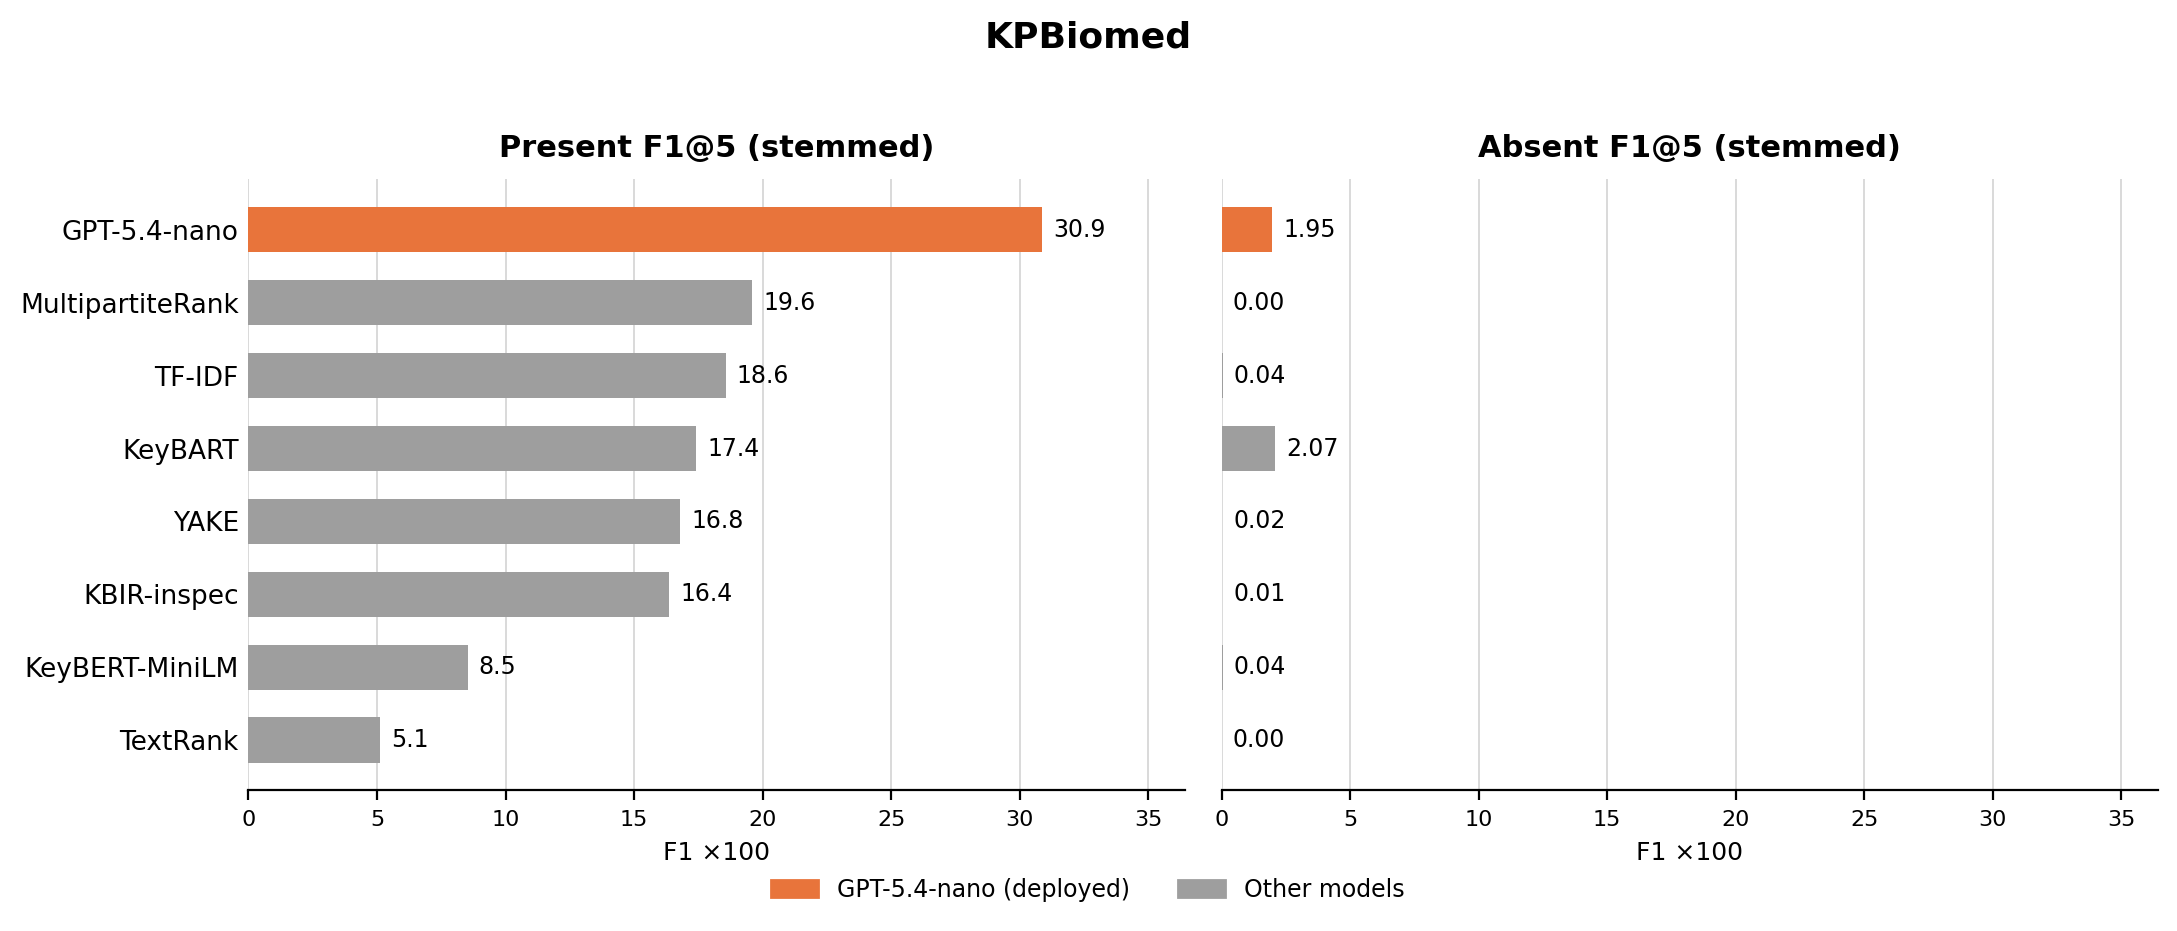
\includegraphics[width=\textwidth]{images/data_and_results/keyword_kpbiomed.png}
\caption{KPBiomed keyword extraction, present and absent F1@5 by model with stemming. The deployed model GPT-5.4-nano is shown in orange and the remaining baselines in grey.}
\label{fig:kw-kpbiomed}
\end{figure*}

\begin{figure*}[t]
\centering
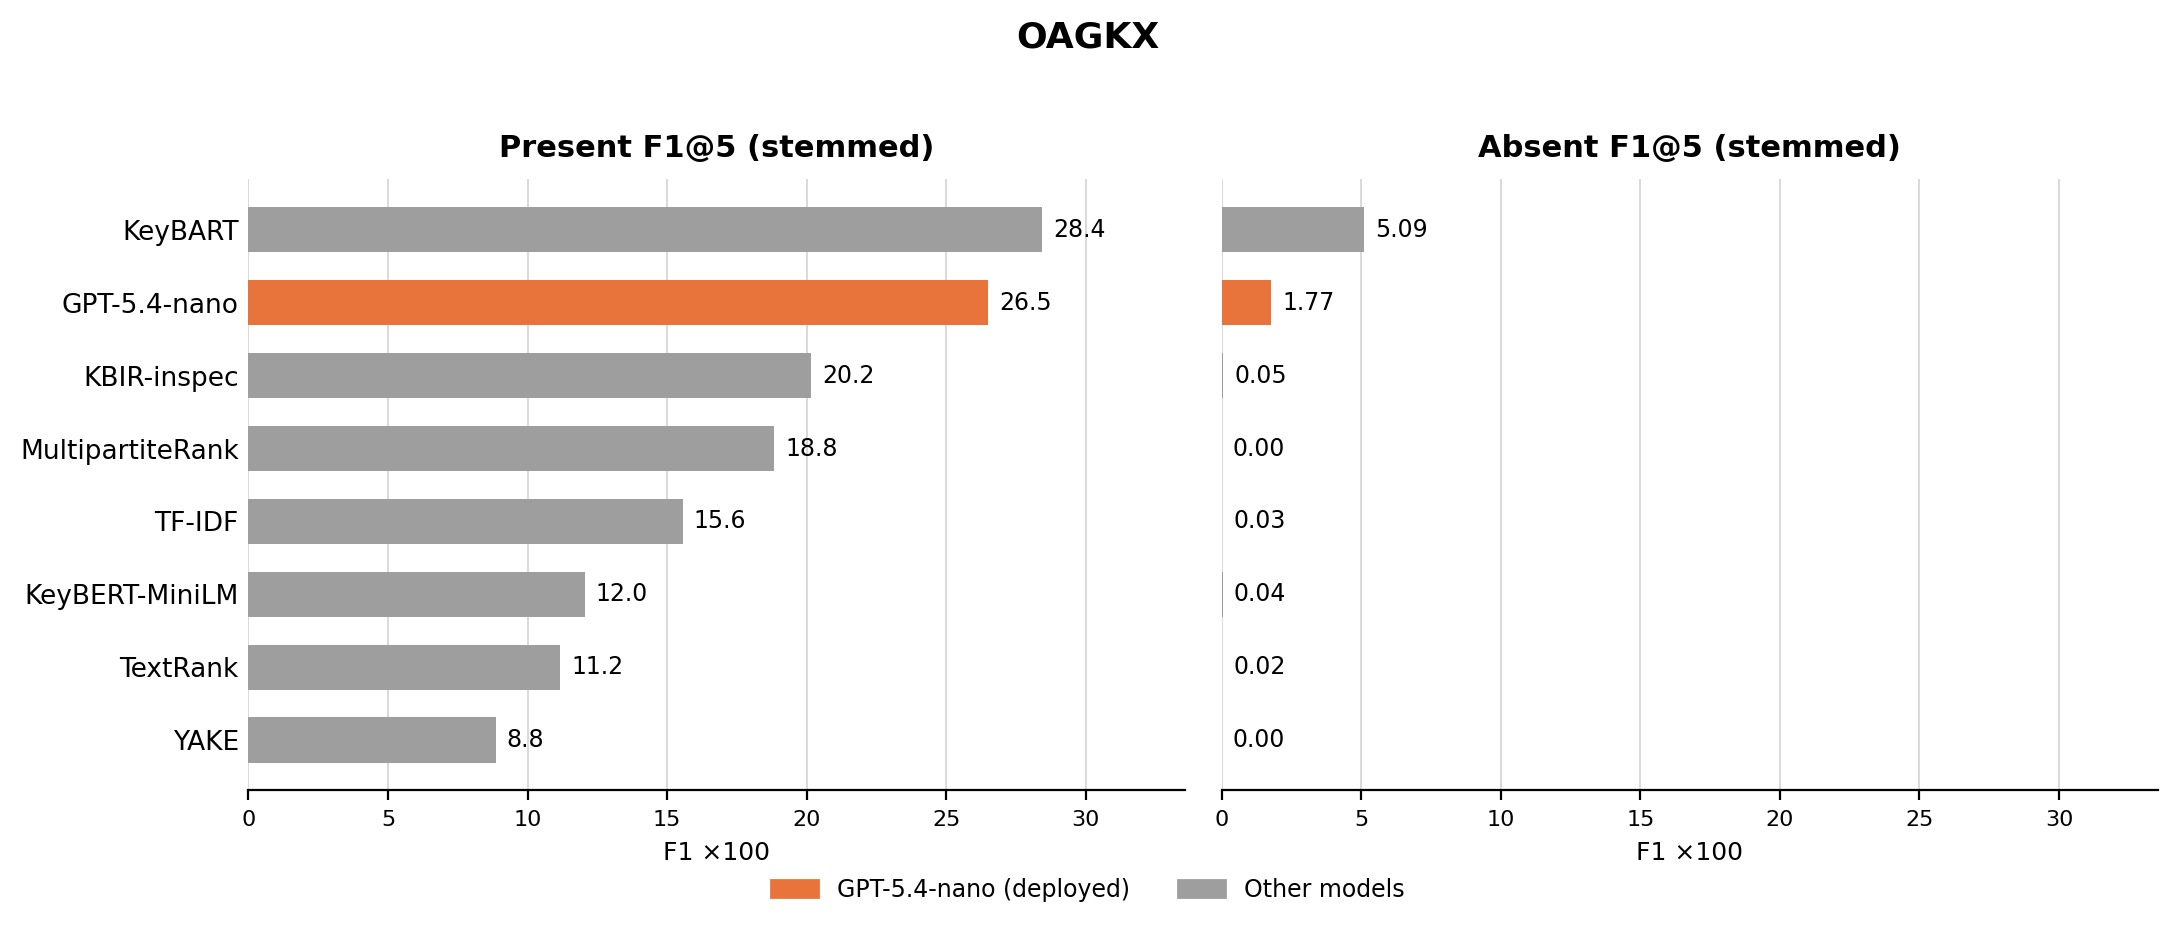
\includegraphics[width=\textwidth]{images/data_and_results/keyword_oagkx.png}
\caption{OAGKX keyword extraction, present and absent F1@5 by model with stemming. The deployed model GPT-5.4-nano is shown in orange and the remaining baselines in grey.}
\label{fig:kw-oagkx}
\end{figure*}

\begin{figure*}[t]
\centering
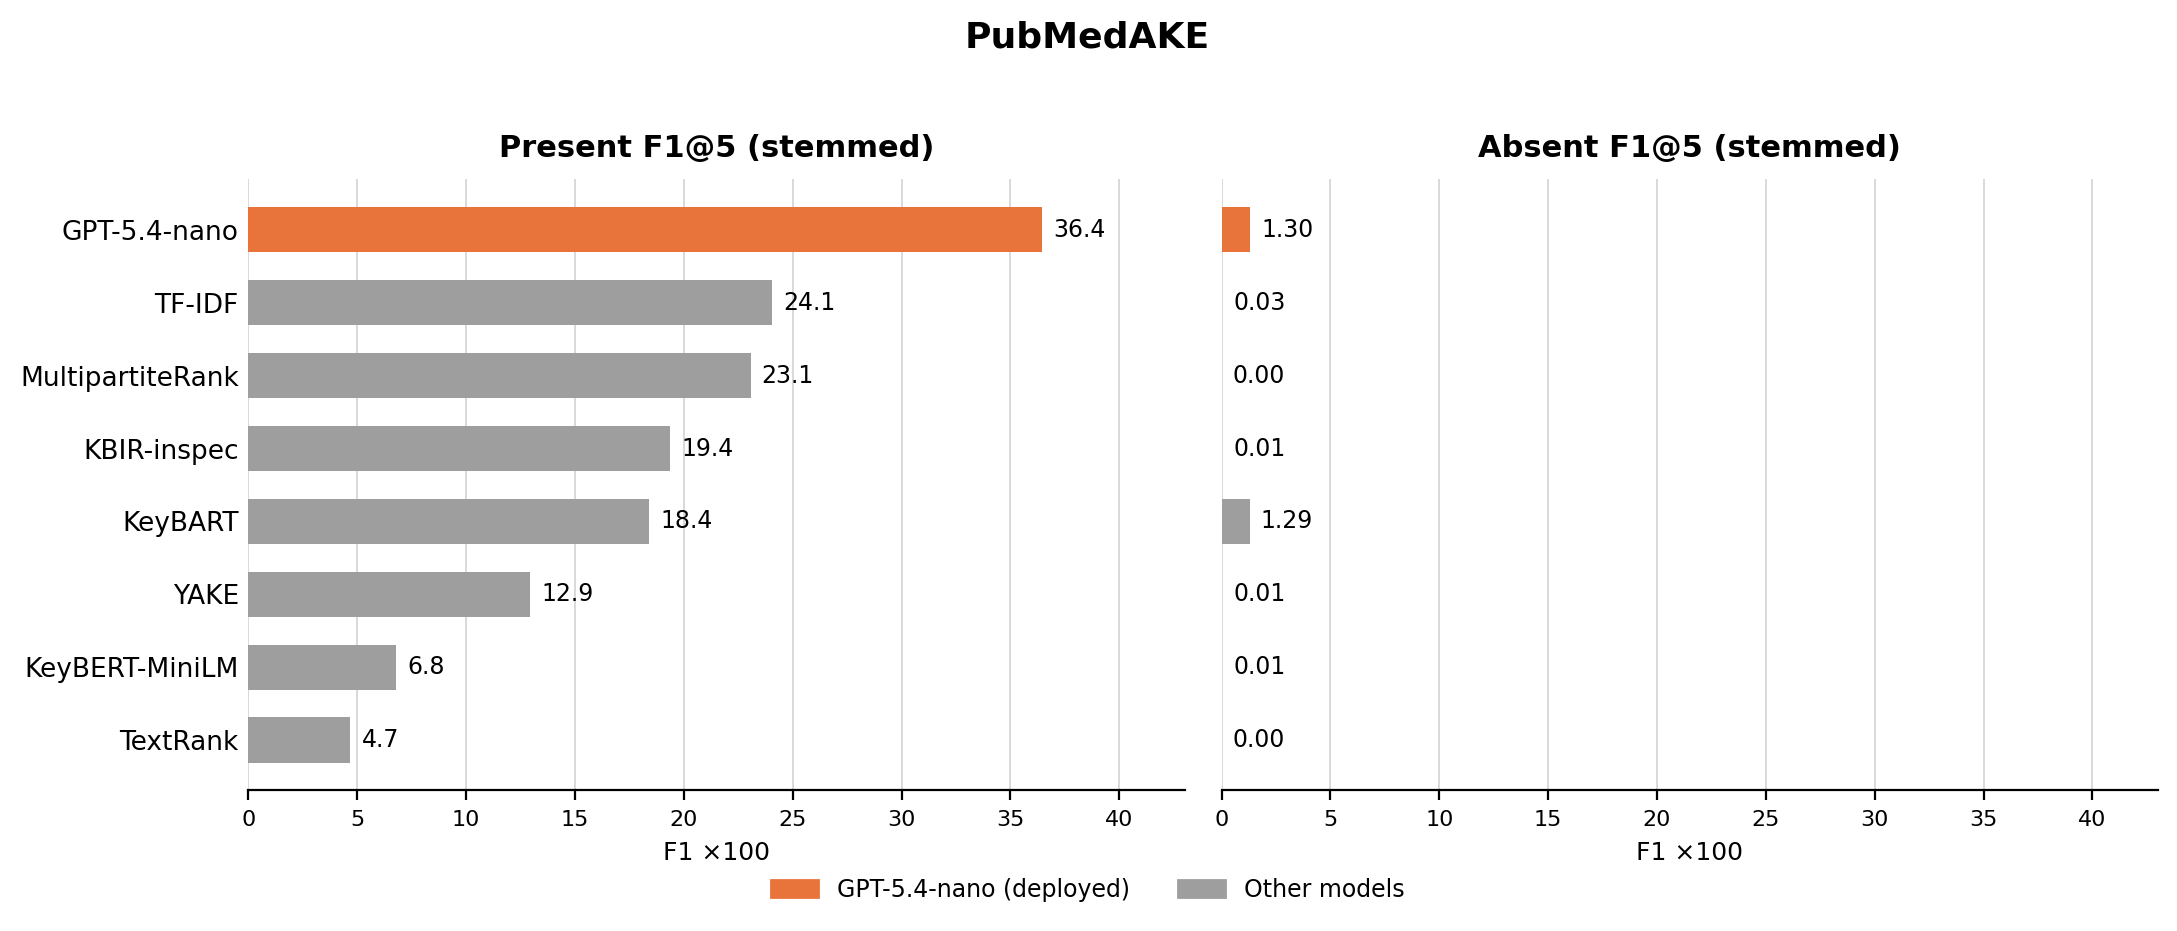
\includegraphics[width=\textwidth]{images/data_and_results/keyword_pubmedake.png}
\caption{PubMedAKE keyword extraction, present and absent F1@5 by model with stemming. The deployed model GPT-5.4-nano is shown in orange and the remaining baselines in grey.}
\label{fig:kw-pubmedake}
\end{figure*}

% --- Natural-language-to-IR accuracy (was Table IX) --------------------------
\begin{table*}[t]
\caption{Natural-language-to-IR accuracy by model. Joint IR accuracy counts a query as correct when both its entities and its Boolean expression are correct under exact matching, reported in the as-deployed or best configuration for each model.}
\label{tab:ir-accuracy}
\centering
\footnotesize
\begin{tabular}{@{}lllcc@{}}
\toprule
Model & Host & Configuration & IR accuracy & 95\% CI \\
\midrule
\textbf{gpt-5.4-nano} & Azure & default, 0 reasoning tok & \textbf{0.937}$^{\dagger}$ & [0.897, 0.983] \\
gpt-5-mini & Azure & default, 384 reasoning tok & 0.931 & [0.879, 0.974] \\
qwen3:8b & Local (Q4) & single-shot & 0.802 & [0.733, 0.871] \\
qwen3:4b & Local (Q4) & thinking$^{\ddagger}$ & 0.784 & [0.707, 0.862] \\
qwen2.5:3b & Local (Q4) & non-reasoning & 0.207 & [0.138, 0.284] \\
phi4-mini & Local (Q4) & non-reasoning & 0.052 & [0.017, 0.095] \\
llama3.2:3b & Local (Q4) & non-reasoning & 0.026 & [0.000, 0.060] \\
\bottomrule
\end{tabular}

\vspace{3pt}
\begin{minipage}{\linewidth}
\footnotesize\itshape
Confidence intervals are 95 percent bootstrap over 1000 iterations. Cross-model gaps that fall within these intervals are treated as ties, and bold marks the deployed model. The dagger denotes a three-run mean, whose single-run range is 0.931 to 0.940, with temperature zero returning a byte-identical output on 96.6 percent of queries (Table~\ref{tab:ir-stability}). The double dagger denotes qwen3:4b, whose single-shot configuration produced degenerate empty output, so its thinking configuration is its only usable score.
\end{minipage}
\end{table*}

% --- Dense bi-encoder full scores (was Table XIV) ---------------------------
\begin{table*}[t]
\caption{Dense bi-encoder retrieval on SciRepEval ad-hoc search, nDCG $\times$100 with 95 percent bootstrap confidence intervals.}
\label{tab:bienc-results}
\centering
\scriptsize
\setlength{\tabcolsep}{4pt}
\begin{tabular}{@{}p{3.0cm}llll@{}}
\toprule
Model & NFCorpus & TREC-CoVID & Search & Average \\
\midrule
Qwen3-Embedding-4B (int8) & \textbf{80.02 [77.75, 82.17]} & \textbf{94.28 [92.96, 95.43]} & 75.54 [74.93, 76.17] & \textbf{83.28 [82.35, 84.19]} \\
EmbeddingGemma-300M & 79.13 [76.84, 81.29] & 92.45 [90.68, 94.03] & 75.32 [74.66, 75.93] & 82.30 [81.32, 83.31] \\
Qwen3-Embedding-0.6B & 77.94 [75.75, 80.22] & 93.90 [92.52, 95.10] & 75.03 [74.41, 75.65] & 82.29 [81.32, 83.25] \\
text-embedding-3-small (existing) & 78.78 [76.61, 81.05] & 92.38 [90.58, 93.96] & 75.14 [74.52, 75.74] & 82.10 [81.08, 83.05] \\
mxbai-embed-large-v1 & 79.37 [77.19, 81.72] & 91.77 [90.02, 93.25] & 74.92 [74.29, 75.56] & 82.02 [81.06, 82.96] \\
SPECTER2-adhoc-query & 70.46 [68.01, 72.97] & 90.08 [87.84, 92.13] & \textbf{78.22 [77.60, 78.86]} & 79.59 [78.46, 80.71] \\
BGE-M3 & 74.05 [71.72, 76.35] & 89.21 [87.08, 91.16] & 74.82 [74.20, 75.46] & 79.36 [78.29, 80.42] \\
SPECTER2-base (existing) & 72.03 [69.60, 74.54] & 89.46 [86.99, 91.58] & 73.76 [73.12, 74.41] & 78.42 [77.27, 79.58] \\
\bottomrule
\end{tabular}

\vspace{3pt}
\begin{minipage}{\linewidth}
\footnotesize\itshape
The metric is SciRepEval ad-hoc-search full-ranking nDCG over a per-query candidate pool, not BEIR full-corpus nDCG@10. Confidence intervals are 95 percent bootstrap [lo, hi] over 1000 iterations with seed 42, and bold marks the best point estimate per column. On Average the top five models' intervals overlap, a statistical tie, and SPECTER2-adhoc-query's Search lead is the one between-model gap whose interval clears the general models.
\end{minipage}
\end{table*}

% --- Cross-encoder full scores (was Table XVI) ------------------------------
\begin{table*}[t]
\caption{Cross-encoder re-ranking on SciRepEval ad-hoc search, nDCG $\times$100 with 95 percent bootstrap confidence intervals, sorted by Average.}
\label{tab:xenc-results}
\centering
\scriptsize
\setlength{\tabcolsep}{4pt}
\begin{tabular}{@{}p{3.2cm}llll@{}}
\toprule
Model (scorer) & NFCorpus & TREC-CoVID & Search & Average \\
\midrule
Cohere Rerank 4.0 Pro (API) & \textbf{80.42 [78.17, 82.60]} & \textbf{94.60 [93.30, 95.71]} & 75.39 [74.76, 76.00] & \textbf{83.47 [82.54, 84.33]} \\
Qwen3-Reranker-4B (int8) & 80.10 [77.94, 82.14] & 94.37 [92.90, 95.60] & 74.93 [74.32, 75.56] & 83.13 [82.18, 83.99] \\
Cohere Rerank 4.0 Fast (API) & 78.77 [76.55, 80.98] & 94.15 [92.83, 95.31] & \textbf{75.42 [74.75, 76.04]} & 82.78 [81.83, 83.68] \\
Qwen3-Reranker-0.6B (fp16) & 78.06 [75.65, 80.24] & 93.98 [92.59, 95.20] & 75.25 [74.59, 75.85] & 82.43 [81.50, 83.34] \\
mxbai-rerank-large-v1 (435M) & 78.32 [76.08, 80.76] & 91.50 [89.43, 93.33] & 74.78 [74.15, 75.46] & 81.53 [80.48, 82.59] \\
jina-reranker-v2-base (278M) & 76.73 [74.49, 79.01] & 91.84 [90.05, 93.52] & 75.37 [74.73, 75.99] & 81.31 [80.28, 82.30] \\
MedCPT-Cross-Encoder (109M, biomed) & 75.70 [73.21, 78.03] & 88.91 [86.61, 90.97] & 73.97 [73.34, 74.63] & 79.53 [78.40, 80.66] \\
ms-marco-MiniLM-L-6-v2 (22M) & 73.10 [70.78, 75.48] & 88.78 [86.41, 90.90] & 75.21 [74.58, 75.84] & 79.03 [77.90, 80.13] \\
bge-reranker-v2-m3 (568M) & 70.71 [68.31, 73.07] & 90.30 [88.29, 92.18] & 74.40 [73.78, 75.05] & 78.47 [77.37, 79.53] \\
ms-marco-MiniLM-L-12-v2 (33M) & 69.88 [67.41, 72.38] & 87.17 [84.73, 89.52] & 75.09 [74.44, 75.71] & 77.38 [76.17, 78.54] \\
bge-reranker-large (560M) & 66.49 [64.11, 68.85] & 87.27 [84.61, 89.62] & 74.22 [73.59, 74.85] & 76.00 [74.80, 77.16] \\
bge-reranker-base (278M) & 58.75 [56.38, 60.94] & 84.98 [82.12, 87.60] & 72.60 [71.97, 73.24] & 72.11 [70.84, 73.35] \\
gte-reranker-modernbert-base (150M) & 48.88 [46.82, 50.93] & 79.03 [76.40, 81.60] & 69.94 [69.26, 70.60] & 65.95 [64.91, 67.07] \\
\bottomrule
\end{tabular}

\vspace{3pt}
\begin{minipage}{\linewidth}
\footnotesize\itshape
The metric is SciRepEval ad-hoc-search full-ranking nDCG over a reranking pool, not BEIR full-corpus nDCG@10. Confidence intervals are 95 percent bootstrap [2.5 percent, 97.5 percent] over 1000 iterations with seed 42, with the Average resampled independently within each dataset. The intervals are tight on Search, which has 2585 queries, and wide on TREC-CoVID, which has 50, and bold marks the best point estimate per column. The top four models, namely Cohere Pro, Qwen3-Reranker-4B, Cohere Fast, and Qwen3-Reranker-0.6B, have heavily overlapping Average intervals and form a statistical tie, within which the best self-hostable model, Qwen3-Reranker-4B at int8, is tied with Cohere Pro. On Search the small candidate pool saturates every reranker at around 75. For reference, the bi-encoder embeddings without intervals give the best embedder Qwen3-Embedding-4B at 83.28 Average, SPECTER2-adhoc-query at 78.22 on Search, which is above every reranker here, and text-embedding-3-small at 82.10 Average.
\end{minipage}
\end{table*}

% Flush all appendix floats before the document ends / any column-mode change.
\clearpage          % Appendix A
% ============================================================================
%  Appendix B: Worked Example (Query, IR, Compiled Cypher)  --  PLACEHOLDER
%  Body-only file. \input after \appendix in main.tex, so \section{Title} auto-
%  prints "Appendix B: Title" (custom patch in preamble.sty:307) and \label{app:worked}
%  resolves to the letter via \ref. research_design.tex cites it as
%  Appendix~\ref{app:worked}.
%
%  AUTHOR TODO: replace the [In preparation.] note below with the worked example
%  (natural-language query, its normalised form, the extracted IR, and the
%  compiled Cypher), as promised in Section~\ref{subsec:component-design}.
% ============================================================================
\section{Worked Example: Query, Intermediate Representation, and Compiled Cypher}
\label{app:worked}

\textit{[In preparation.]}
  % Appendix B (placeholder)
% =============================================================================
%  Appendix C: Prompts and Tool Schemas
%  Body-only section file: no \documentclass, no \begin{document}; \input it.
%
%  WIRING (already done in this repo; recorded here for reference):
%   (a) PREAMBLE: listings is already loaded (matlab-prettifier pulls it in; see
%       preamble.sty comment "matlab-prettifier already loads the listings
%       package"), so no \usepackage{listings} line was added. The \lstset below
%       is self-contained and supplies all configuration this file needs.
%   (b) MAIN.TEX: after \appendix (which activates the custom \section patch in
%       preamble.sty:307), this file is \input as the third appendix, so its
%       \section{Prompts and Tool Schemas} auto-prints "Appendix C: ..." and the
%       \label below resolves to the letter "C". Reordering the \input list
%       relettering everything automatically.
%   (c) CROSS-REFERENCES: research_design.tex refers here via Appendix~\ref{app:prompts}
%       (dynamic), so the letter always matches this appendix's position.
%
%  FIDELITY: every prompt / schema below is reproduced VERBATIM from source.
%  Nothing was corrected. British spellings ("recognised") and any wording that
%  reads like a typo are intentional and left exactly as in the code.
%
%  REDACTIONS: secret-shaped values are replaced by clearly-marked placeholders
%  (<AZURE_OPENAI_ENDPOINT>, <AZURE_OPENAI_API_KEY>). No real keys/endpoints
%  appear in this file. (A live key is committed in the source repo's .env and
%  .env.example; flagged separately to the author. It is NOT reproduced here.)
%
%  RENDERING: the appendix region is \onecolumn, so the listings below are plain
%  (non-floating) lstlisting blocks; they already span the full text width and,
%  unlike figure*, break cleanly across pages (the extraction and IR prompts are
%  too long to fit a single float). If you restore two-column appendices, wrap
%  the (short) JSON tool schema in figure* to span both columns, but keep the
%  long prompt listings unfloated so they can page-break.
% =============================================================================

\lstset{
  basicstyle=\ttfamily\footnotesize,
  breaklines=true,
  frame=single,
  columns=fullflexible,
  keepspaces=true,
  showstringspaces=false,
  upquote=true,
  extendedchars=true,
  % The one non-ASCII char in the reproduced prompts is a U+2014 em-dash (in the
  % IR system prompt). The document uses OT1 Computer Modern (no fontenc/lmodern
  % in preamble.sty), where \textemdash inside \ttfamily wrongly prints "|", so
  % force the roman em-dash glyph to keep the reproduction faithful.
  literate={—}{{\normalfont\textemdash}}1
}

% Dynamic heading: \appendix (main.tex) makes this print "Appendix C: Prompts and
% Tool Schemas" and adds its own ToC entry; \label resolves to the letter via \ref.
\section{Prompts and Tool Schemas}
\label{app:prompts}

This appendix reproduces, verbatim, the language-model prompts and the forced
tool-call schema used by the two generation stages evaluated in this report: the
keyword-generation module (Section~\ref{sec:research-design}) and the
natural-language-to-Intermediate-Representation (NL$\rightarrow$IR) extractor.

% -----------------------------------------------------------------------------
\subsection*{Keyword-generation prompt and configuration}
% -----------------------------------------------------------------------------

The keyword module sends a fixed system prompt plus a per-work user message to an
Azure OpenAI \texttt{gpt-5.4-nano} deployment and parses a JSON array of
keyphrases from the completion. The system prompt reproduced below is the
original \emph{extraction} variant (\lstinline|prompt_variant: extraction|), which
is the deployed procedure vendored from production and the one described in the
report body.

% NOTE (explicit, not silent): the source config.yaml currently sets
%   prompt_variant: generation_tight   (a benchmark-only "Run B" refinement whose
% text lives in prompts.json -> "generation_system"). Two further variants exist
% in code (extraction | generation | generation_tight). Per the author's decision
% only the original *extraction* prompt is reproduced here; the generation
% variants are not.

\begin{lstlisting}
Extract the most relevant keywords from the provided scientific text for search and indexing purposes and return them as a JSON list.

Include only technical terms, concepts, or phrases central to the content of the text. Avoid generic or overly broad words unless they are critical to the subject matter. Ensure that the extracted keywords are concise and representative of the scientific content.

# Steps

1. Analyze the provided scientific text for its primary topics, concepts, and technical terms.
2. Identify specific keywords or phrases that summarize the main ideas or are important for searchability.
3. Remove any non-specific, redundant, or irrelevant terms (e.g., articles, conjunctions, or overly generic terms like "studies" or "research").
4. Return the extracted keywords as a JSON array.

# Output Format

```json
[
    "keyword1",
    "keyword2",
    "...",
    "keywordN"
]
```

# Examples

**Input:**
"Photosynthesis is the process by which green plants and some other organisms use sunlight to synthesize foods with the aid of chlorophyll pigments and carbon dioxide. Plants absorb carbon dioxide (CO2) from the atmosphere and water (H2O) from the soil to produce glucose and oxygen (O2). The process involves the transformation of light energy into chemical energy stored in glucose molecules."

**Output:**
```json
[
    "photosynthesis",
    "green plants",
    "chlorophyll pigments",
    "carbon dioxide",
    "glucose",
    "oxygen",
    "light energy",
    "chemical energy"
]
```

**Input:**
"The human genome is composed of approximately 3 billion base pairs of DNA, containing the instructions for building and maintaining an organism. Genes, made of DNA, encode proteins, which perform most of the work in cells. Genomic sequencing methods have advanced significantly, allowing for a better understanding of the genetic basis of diseases and traits."

**Output:**
```json
[
    "human genome",
    "base pairs",
    "DNA",
    "genes",
    "proteins",
    "genomic sequencing",
    "genetic basis"
]
```
\end{lstlisting}

\noindent The user message is a one-line template; the system prompt has no
interpolation slots (the \lstinline|.format(n=n)| call at the call site is a
no-op for this variant, since it contains no braces):

\begin{lstlisting}
Text:
{text}
\end{lstlisting}

\noindent The single slot \lstinline|{text}| is filled with the work's title and
abstract joined as \lstinline|"{title}\n\n{abstract}"|, passed through one
citation-cleaning pass and truncated to \texttt{max\_text\_chars} $=6000$
characters before sending.

\medskip
\noindent Exact call configuration (from code; parameters marked
\texttt{[REDACTED]} are secret-shaped and replaced by placeholders):

\begin{lstlisting}
API                   : AsyncAzureOpenAI(...).chat.completions.create(...)
model  (deployment)   : cfg["deployment"]
                        <- env AZURE_OPENAI_DEPLOYMENT  (Azure gpt-5.4-nano deployment)
                        <- config.yaml value: "<AZURE_DEPLOYMENT>"  (placeholder)
                        <- code fallback default: "gpt-5.4-nano"
temperature           : 0.0
max_completion_tokens : 400            (config.yaml; code fallback 300)
api_version           : "2024-12-01-preview"
azure_endpoint        : <AZURE_OPENAI_ENDPOINT>   [REDACTED: internal URL, from env/.env]
api_key               : <AZURE_OPENAI_API_KEY>    [REDACTED: env only, never in code]
top_p, seed, n,
response_format,
reasoning_effort,
tool_choice           : (not sent; left at API defaults)

Client / retries      : AzureOpenAI client max_retries = 0; custom backoff with
                        max_retries = 8, empty_retries = 2 (not API parameters)
Output/parsing caps   : max_keywords (n) = 20; max_text_chars = 6000
\end{lstlisting}

\noindent\textit{Provenance. Source:}
\lstinline|keyword_benchmark/benchmark/reference/extract_keywords.py|
\textit{, system prompt} \lstinline|_SYSTEM_PROMPT| \textit{lines 37--94, user
template} \lstinline|_USER_PROMPT| \textit{line 96, live call site lines
345--387; call parameters from} \lstinline|benchmark/config.yaml| \textit{and}
\lstinline|_load_azure_config()| \textit{lines 183--202. Working copy}
\lstinline|/home/jordanguyot/homeserver/lk_ws/keyword_benchmark| \textit{is not a
git repository, so no commit hash is available (file dated 2026-06-04); the
version-controlled upstream is} \lstinline|litview-keyword-benchmark| \textit{and
the extraction procedure itself is vendored from production} \lstinline|litview-kg|\textit{.}

% -----------------------------------------------------------------------------
\subsection*{IR-extraction system prompt}
% -----------------------------------------------------------------------------

The normalised natural-language query is converted to the Intermediate
Representation by a single forced tool call. The system prompt below is sent as
the \texttt{system} message; the \texttt{user} message is the raw (already
normalised) query string, with no additional templating.

% PRODUCTION-PARITY FLAG (do not silently treat as the production prompt):
% This prompt is VENDORED AND ADAPTED (trimmed) from the production extractor
% litview-qapi/api/pipeline/extract.py :: LLMExtractor. It is NOT byte-identical
% to production. Kept: the build_works_search_ir forced tool call + expression
% shape-normalisation. Dropped from production: quoted/exact-phrase marking,
% casing normalisation, confidence gating, and the OR-fallback; the prompt is
% trimmed to the benchmark's "boolean-core" scope and routes year/type/etc. to
% the (ignored) filter fields. See DECISIONS.md D21 and README.md in the
% nl_to_ir_benchmark repo. The version below is the benchmark (homeserver) copy.

\begin{lstlisting}
You are a search-intent extractor for an academic literature knowledge graph.
Given a natural-language query, call the build_works_search_ir tool to extract the BOOLEAN
CORE of the query: a typed list of entities and a boolean expression tree over them.

Entity types:
- "keyword": a concept, technique, method, disease, or topic. A single recognised name is ONE
  keyword even if multi-word (e.g. "single-cell RNA sequencing", "CAR-T cell therapy",
  "gut microbiome", "CRISPR-Cas9"). A phrase naming two separable concepts is split into
  separate keywords (e.g. "deep learning for medical imaging" -> "deep learning" AND
  "medical imaging").
- "person": author names. Use the COMPLETE name exactly as given; never split or truncate
  hyphenated surnames. Exactly one person entity per author mentioned.
- "venue": journal/conference names (cue: "published in <venue>").
- "institution": universities, labs, research institutes (cue: "from the <institution>").

Expression tree (how the entities combine):
- Leaf: {"node_type": "entity_ref", "idx": <index into entities>}
- Boolean: {"node_type": "bool_expr", "op": "and"|"or"|"not", "children": [...]}; NOT has
  exactly 1 child, AND/OR have 2+ children.
- Single entity -> {"node_type": "entity_ref", "idx": 0}.
- Concepts that must co-occur -> AND. Alternatives ("or", "either ... or") -> OR.
- Exclusion ("not X", "excluding X", "but not X") -> include X as an entity and wrap its ref
  in NOT inside an AND with the positive entities. When a SUBTYPE is excluded ("stem cells but
  not embryonic"), the negated entity is the specific subtype ("embryonic stem cells").
- Respect grouping/precedence: "(A or B) and C" -> AND(OR(ref_A, ref_B), ref_C), NOT
  OR(ref_A, AND(ref_B, ref_C)).

Out of scope — DO NOT add these as entities or to the expression. If present, route them to
the filters/limit/order_by fields (they are ignored downstream), never as keyword entities:
- year/date ranges ("since 2020"), work type, open-access status, citation thresholds,
  title substrings, sorting, and result-count limits.

Extract exactly what the query states. Do not invent entities.
\end{lstlisting}

\noindent The call forces this single tool with
\lstinline|tool_choice={"type": "function", "function": {"name": "build_works_search_ir"}}|,
sending \lstinline|max_completion_tokens=2048|; \texttt{temperature} is sent only
when non-zero (default \texttt{0.0}, so omitted), as \texttt{gpt-5} reasoning
deployments reject a non-default temperature.

\medskip
\noindent\textit{Provenance. Source:}
\lstinline|nl_to_ir_benchmark/nl2ir_eval/azure_extractor.py|\textit{,}
\lstinline|_SYSTEM_PROMPT| \textit{lines 104--138, forced-tool call site (}\lstinline|_call_model|\textit{)
lines 247--267. Working copy}
\lstinline|/home/jordanguyot/homeserver/lk_ws/nl_to_ir_benchmark| \textit{is not a
git repository, so no commit hash is available (file dated 2026-06-23). This is
the benchmark copy, adapted/trimmed from the production extractor}
\lstinline|litview-qapi/api/pipeline/extract.py :: LLMExtractor| \textit{(see}
\lstinline|DECISIONS.md| \textit{D21); it is not byte-identical to the deployed
production prompt.}

% -----------------------------------------------------------------------------
\subsection*{IR tool schema}
% -----------------------------------------------------------------------------

The IR extractor forces the model to call a single function,
\lstinline|build_works_search_ir|, whose parameter schema mirrors the
Intermediate Representation. The complete tool definition sent to the API is
reproduced below as JSON (reconstructed from the source Python literal: the
schema reference is inlined and the multi-line \lstinline|description| strings
are concatenated exactly as Python joins them at runtime). Only the
\lstinline|entities| and \lstinline|expression| fields are scored; the
\lstinline|filters|, \lstinline|limit| and \lstinline|order_by| fields exist so
the model routes out-of-scope constraints there instead of inventing keyword
entities.

\begin{lstlisting}[language=]
{
  "type": "function",
  "function": {
    "name": "build_works_search_ir",
    "description": "Extract structured search intent from a natural-language query about academic works. Return the typed entity list and the boolean expression tree combining them.",
    "parameters": {
      "type": "object",
      "properties": {
        "entities": {
          "type": "array",
          "items": {
            "type": "object",
            "properties": {
              "type": {
                "type": "string",
                "enum": ["keyword", "person", "venue", "institution"]
              },
              "value": { "type": "string" },
              "confidence": { "type": "number", "minimum": 0.0, "maximum": 1.0 }
            },
            "required": ["type", "value", "confidence"]
          }
        },
        "expression": {
          "description": "Boolean expression tree defining how entities combine. Leaf nodes: {\"node_type\": \"entity_ref\", \"idx\": <int>} referencing entities by index. Interior nodes: {\"node_type\": \"bool_expr\", \"op\": \"and\"|\"or\"|\"not\", \"children\": [...]}. NOT must have exactly 1 child. AND/OR must have 2+ children. For a single entity, use {\"node_type\": \"entity_ref\", \"idx\": 0}.",
          "type": "object"
        },
        "filters": {
          "type": "object",
          "properties": {
            "year": {
              "type": "object",
              "properties": {
                "gte": { "type": "integer" },
                "lte": { "type": "integer" }
              }
            },
            "type": { "type": "array", "items": { "type": "string" } },
            "open_access_status": { "type": "array", "items": { "type": "string" } },
            "citation_count": {
              "type": "object",
              "properties": { "gte": { "type": "integer", "minimum": 0 } }
            },
            "title_contains": { "type": "string" }
          }
        },
        "limit": { "type": "integer", "minimum": 1, "maximum": 100 },
        "order_by": {
          "type": "string",
          "enum": ["relevance", "most_recent", "oldest", "most_cited", "least_cited"]
        }
      },
      "required": ["entities", "expression"]
    }
  }
}
\end{lstlisting}

\noindent\textit{Provenance. Source:}
\lstinline|nl_to_ir_benchmark/nl2ir_eval/azure_extractor.py|\textit{,}
\lstinline|_EXTRACTION_TOOL| \textit{(function wrapper) lines 91--101 and}
\lstinline|_EXTRACTION_TOOL_SCHEMA| \textit{(parameters) lines 47--89. Working
copy} \lstinline|/home/jordanguyot/homeserver/lk_ws/nl_to_ir_benchmark|
\textit{is not a git repository (file dated 2026-06-23); the schema "mirrors the
production WorksSearchIR".}
         % Appendix C
% ============================================================================
%  Appendix D: Error Exemplars
%  Body-only file. \input after \appendix in main.tex, so \section{Title} auto-
%  prints "Appendix D: Title" (custom patch in preamble.sty:307) and \label{app:errors}
%  resolves to the letter via \ref. analysis_and_discussion.tex cites it as
%  Appendix~\ref{app:errors} at two points: the keyword-generation exemplar
%  (Section V-A1) and the filter_distractor exemplar (Section V-A2).
%
%  FIDELITY: every source text, predicted keyphrase list, query, and IR below is
%  reproduced VERBATIM from the benchmark artefacts. Model output is shown exactly
%  as returned (no reordering, no de-duplication, no correction). Provenance notes
%  give the source file for every record, matching the convention of Appendix C.
%
%  LISTINGS: this file relies on the \lstset defined in Appendix C (same document
%  scope under \input). If Appendix D is ever moved before Appendix C, lift the
%  \lstset block from appendix_c_prompts.tex to before the first lstlisting here.
% ============================================================================

% Dynamic heading: \appendix (main.tex) makes this print "Appendix D: Error
% Exemplars" and adds its own ToC entry; \label resolves to the letter via \ref.
\section{Error Exemplars}
\label{app:errors}

This appendix reproduces the two failure exemplars referenced from the analysis:
one from the keyword-generation module (Section~\ref{subsec:rq1}) and one from the
natural-language-to-IR extractor (Section~\ref{subsec:rq1}). Each is drawn
verbatim from the benchmark run reported in Section~\ref{sec:data-results}, with
its source record cited. Both illustrate the characteristic behaviour of a
language model asked to produce a structured artefact, namely a keyphrase that
leaves the source text, and a filter term miscategorised as a searchable entity.

% -----------------------------------------------------------------------------
\subsection*{Keyword generation, keyphrases absent from the source text}
% -----------------------------------------------------------------------------

The keyword prompt of Appendix~\ref{app:prompts} asks the model to work mostly by
extraction while also producing a few higher-level keyphrases that need not appear
verbatim (\lstinline|prompt_variant: generation_tight|). The two records below
show the two kinds of absent keyphrase this produces, and correspond to the
present/absent split of Section~\ref{sec:results-keywords}: a legitimately absent
concept that the reference set also lists, and a genuinely spurious concept the
model inferred but that appears in neither the source nor the reference set. Both
are drawn from the deployed \texttt{gpt-5.4-nano} run at temperature zero. In each
record the predicted list is reproduced exactly as returned, and every
absent-from-source verdict is that of the benchmark scorer, which lowercases,
tokenises, Porter-stems, and tests for a contiguous run of stems in the source, so
that no example turns on a stemming or hyphenation artefact.

\medskip
\noindent\textbf{Record 1, an absent keyphrase the reference set also lists.}
PubMedAKE document \lstinline|PMC3647503|. The title and abstract sent to the
model were:

\begin{lstlisting}
Campylobacter coli Outbreak in Men Who Have Sex with Men, Quebec, Canada, 2010-2011

During September 2010-November 2011, a cluster of erythromycin-susceptible, tetracycline- and ciprofloxacin-resistant Campylobacter coli pulsovar 1 infections was documented, involving 10 case-patients, in Montreal, Quebec, Canada. The findings suggested sexual transmission of an enteric infection among men who have sex with men.
\end{lstlisting}

\noindent The model returned the following ranked list (verbatim, fifteen
keyphrases):

\begin{lstlisting}[language=]
["campylobacter coli", "men who have sex with men", "erythromycin-susceptible", "tetracycline-resistant", "ciprofloxacin-resistant", "pulsovar 1", "outbreak", "montreal", "quebec", "sexual transmission", "enteric infection", "2010-2011", "cluster of infections", "pulsovar", "antimicrobial resistance"]
\end{lstlisting}

\noindent Of these, the target keyphrase is \lstinline|antimicrobial resistance|
(rank~14). It appears nowhere in the source text, yet it stem-matches one of the
reference set's own absent keyphrases (\lstinline|antimicrobial resistance|), so
it is a legitimately generated higher-level concept rather than an error, in that
the paper is about resistant infections, and the reference indexer assigned the same
term without it appearing verbatim. This is the behaviour the absent-F1 score of
Section~\ref{sec:results-keywords} is designed to credit. The other fourteen
predictions are present in the source, with the sole further exception of
\lstinline|tetracycline-resistant|, absent only because the source writes
``tetracycline- and ciprofloxacin-resistant'' and the tokens are non-contiguous.

\medskip
\noindent\textbf{Record 2, a spurious keyphrase matching neither source nor
reference.} KPBiomed document \lstinline|33768921|. The title and abstract sent to
the model were:

\begin{lstlisting}
Atypical solid pseudopapillary tumor of the pancreas in a 14-year-old. Diagnostic approach can be difficult in pediatric pancreatic masses. Our case shows that even though radiologic appearance was not conclusive, surgery remains the main treatment in resectable masses especially in children.
\end{lstlisting}

\noindent The model returned the following ranked list (verbatim, ten
keyphrases):

\begin{lstlisting}[language=]
["atypical solid pseudopapillary tumor", "pancreas", "pediatric pancreatic mass", "solid pseudopapillary tumor", "surgery", "resectable mass", "diagnostic approach", "radiologic appearance", "pediatric oncology", "14-year-old"]
\end{lstlisting}

\noindent Here the target keyphrase is \lstinline|pediatric oncology| (rank~8). It
appears nowhere in the source and matches no reference keyphrase, present or
absent. It is a plausible inference from the paper's subject, a paediatric
pancreatic tumour, but it is a concept the model introduced rather than one the
text or the indexer supports, and it is the cleanest single-phrase illustration of
the spurious generation the extraction framing is meant to minimise. The other
nine predictions are present in the source.

\medskip
\noindent Taken together, the two records make the point of the present/absent
split concrete. Record~1's absent keyphrase is the kind the prompt intends and the
metric rewards, whereas Record~2's is the kind it does not. Across the benchmark the
second kind is rare, which is why \texttt{gpt-5.4-nano}'s absent-F1 scores sit in
the low single digits (Section~\ref{sec:results-keywords}) rather than at zero
like the purely extractive baselines or higher like a freely generative one.

% -----------------------------------------------------------------------------
\subsection*{IR extraction, a filter term treated as a searchable entity}
% -----------------------------------------------------------------------------

The largest single source of IR-extraction error is the
\lstinline|filter_distractor| stratum (Section~\ref{sec:results-keywords},
Table~\ref{tab:ir-stratum}), in which the model treats a filter term, such as a
publication-type or open-access constraint, as a keyword entity rather than
routing it to the out-of-scope filter fields the prompt defines
(Appendix~\ref{app:prompts}). The record below is the cleanest of the three
failures in this stratum. The query as sent to the model was:

\begin{lstlisting}[language=]
immunotherapy for melanoma, clinical trials
\end{lstlisting}

\noindent The hand-written gold IR treats ``clinical trials'' as a
publication-type filter, so it drops out of the boolean core, leaving two keyword
entities under an AND:

\begin{lstlisting}[language=]
{
  "entities": [
    {"type": "keyword", "value": "immunotherapy"},
    {"type": "keyword", "value": "melanoma"}
  ],
  "expression": {
    "node_type": "bool_expr", "op": "and",
    "children": [
      {"node_type": "entity_ref", "idx": 0},
      {"node_type": "entity_ref", "idx": 1}
    ]
  }
}
\end{lstlisting}

\noindent The model instead lifted ``clinical trials'' into the entity list as a
third keyword and AND-ed it into the expression:

\begin{lstlisting}[language=]
{
  "entities": [
    {"type": "keyword", "value": "immunotherapy"},
    {"type": "keyword", "value": "melanoma"},
    {"type": "keyword", "value": "clinical trials"}
  ],
  "expression": {
    "node_type": "bool_expr", "op": "and",
    "children": [
      {"node_type": "entity_ref", "idx": 0},
      {"node_type": "entity_ref", "idx": 1},
      {"node_type": "entity_ref", "idx": 2}
    ]
  }
}
\end{lstlisting}

\noindent The two true entities, \lstinline|immunotherapy| and
\lstinline|melanoma|, are both recovered, so entity recall is~1.0, while the
spurious \lstinline|clinical trials| entity drops entity precision to~0.67 and,
because it adds a conjunct the gold expression does not contain, makes the boolean
expression inequivalent, so the query is scored incorrect under the joint measure.
The failure is a categorisation slip rather than a structural one, in that the
model built a well-formed expression but over one entity too many. Its practical
cost is a candidate pool narrowed by a keyword match on ``clinical trials'' where
the design intends a publication-type filter, the behaviour
Section~\ref{subsec:rq1} notes is addressable through prompting that defines filter
terms explicitly. The other two failures in this stratum are of the same kind, an
open-access constraint (\lstinline|fd_03|, ``malaria, open access'') and a
publication-type constraint that the model additionally negated (\lstinline|fd_04|,
``mRNA vaccines published after 2019, but not reviews''), each adding a filter term
to the boolean core as a keyword entity. % Appendix D (placeholder)

\end{document}